% Este documento tem a ver com as partes do LIVRO. 

% Tamanhos
% \tiny
% \scriptsize
% \footnotesize
% \small 
% \normalsize
% \large 
% \Large 
% \LARGE 
% \huge
% \Huge

% Posicionamento
% \centering 
% \raggedright
% \raggedleft
% \vfill 
% \hfill 
% \vspace{Xcm}   % Colocar * caso esteja no começo de uma página. Ex: \vspace*{...}
% \hspace{Xcm}

% Estilo de página
% \thispagestyle{<<nosso>>}
% \thispagestyle{empty}
% \thispagestyle{plain}  (só número, sem cabeço)
% https://www.overleaf.com/learn/latex/Headers_and_footers

% Compilador que permite usar fonte de sistema: xelatex, lualatex
% Compilador que não permite usar fonte de sistema: latex, pdflatex

% Definindo fontes
% \setmainfont{Times New Roman}  % Todo o texto
% \newfontfamily\avenir{Avenir}  % Contexto

\begingroup\thispagestyle{empty}

\begin{tikzpicture}[remember picture,overlay]

\node at (4.6,-8.5)
  {\includegraphics[width=\paperwidth]{img/cthulhu-p1.pdf}};
\end{tikzpicture}
                    
\endgroup
\vfill
\pagebreak

\begingroup\thispagestyle{empty}

\begin{tikzpicture}[remember picture,overlay]

\node at (4.6,-8.5)
  {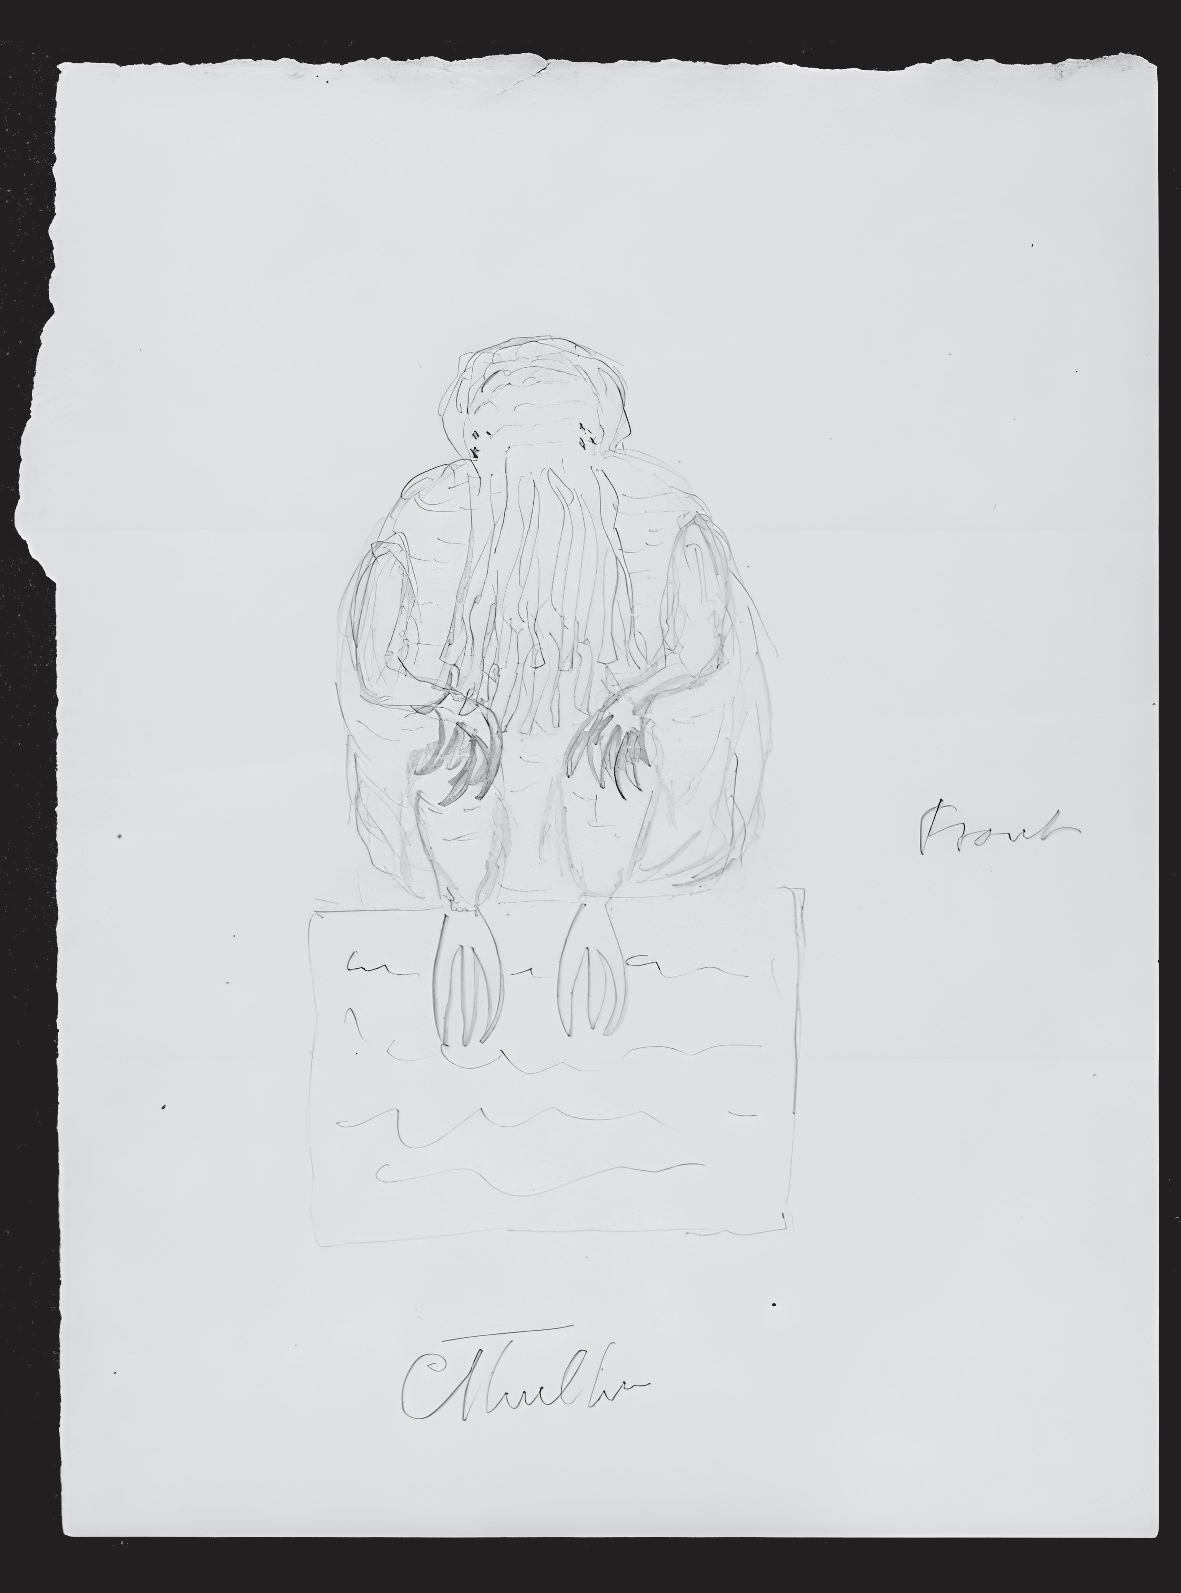
\includegraphics[width=\paperwidth]{img/cthulhu4.pdf}};
\end{tikzpicture}
                    
\endgroup
\vfill
\pagebreak

\begingroup\thispagestyle{empty}\vspace*{.05\textheight} 

              \formular
              \Huge
              \noindent
              \textbf{O chamado\\ de Cthulhu}
              
              {\brabo\LARGE
              \noindent H.\,P. Lovecraft}

\endgroup
\vfill

\begin{flushleft}
	
\includegraphics[width=.3\textwidth]{img/hedra-audio-qr.png}
\end{flushleft}

%\hspace*{-6.5mm}

%\endgroup
%\vfill
%\begin{flushleft}
%    
\includegraphics[width=.3\textwidth]{img/cthulhu_qr.pdf}\\
%    \vspace{-4mm}
%    
\includegraphics[width=.289\textwidth]{img/hedra-audio_logo.png}
%\end{flushleft}
\pagebreak       % [Frontistício]
%\newcommand{\linhalayout}[2]{{\tiny\textbf{#1}\quad#2\par}}
\newcommand{\linha}[2]{\ifdef{#2}{\linhalayout{#1}{#2}}{}}

\begingroup\tiny
\parindent=0cm
\thispagestyle{empty}

%\textbf{copyright}\quad {Nome do autor}\\
\textbf{edição brasileira\,©}\quad			 {Hedra \the\year}\\
\textbf{tradução e introdução\,©}\quad		{Dirceu Villa}\\
%\textbf{organização\,©}\quad			 		 {copyrightorganizacao}\\
%\textbf{ilustração\,©}\quad			 		 {copyrightilustracao}\medskip

\textbf{título original}\quad			 	 {\emph{The Call of Cthulhu}, 1928}\\
%\textbf{edição consultada}\quad			 	 {edicaoconsultada}\\
%\textbf{primeira edição}\quad			 	 {\textit{Pequenos poemas em prosa} (Hedra, 2009)}\\
%\textbf{agradecimentos}\quad			 	 {agradecimentos}\\
%\textbf{indicação}\quad			 			 {indicacao}\medskip

\textbf{edição}\quad			 			 {Jorge Sallum}\\
\textbf{coedição}\quad			 			 {Suzana Salama}\\
\textbf{assistência editorial}\quad			 {Paulo Henrique Pompermaier}\\
%\textbf{revisão}\quad			 			 {}\\
%\textbf{preparação}\quad			 		 {preparacao}\\
%\textbf{iconografia}\quad			 		 {iconografia}\\
\textbf{capa}\quad			 				 {Lucas Kröeff}\medskip
%\textbf{imagem da capa}\quad			 	 {imagemcapa}\medskip

\textbf{ISBN}\quad			 				 {978-85-7715-648-1}\smallskip

% \hspace{-5pt}\begin{tabular}{ll}
% \textbf{conselho editorial} & Adriano Scatolin,  \\
% 							& Antonio Valverde,  \\
% 							& Caio Gagliardi,    \\
% 							& Jorge Sallum,      \\
% 							& Ricardo Valle,     \\
% 							& Tales Ab'Saber,    \\
% 							& Tâmis Parron      
% \end{tabular}

\bigskip

%  \begin{minipage}{7cm}
% \textbf{Dados Internacionais de Catalogação na Publicação (CIP)\\
% (Câmara Brasileira do Livro, SP, Brasil)}

% \textbf{\hrule}\smallskip

% Baudelaire, Charles, 1821--1867\\

% Pequenos poemas em prosa / Charles Baudelaire ; tradução Dorothée de Bruchard. 
% --- 2. ed. --- São Paulo, \textsc{sp}: Editora Hedra, 2023.\\

% Título original: Petits poèmes en prose\\
% \textsc{isbn} 978-85-7715-755-6\\

% 1. Poesia francesa I. Título.\\

% 23-172905 \hfill \textsc{cdd}: 841

% \textbf{\hrule}\smallskip

% \textbf{Elaborado por Eliane de Freitas Leite (CRB 8/8415)}\\
% \\

% \textbf{Índices para catálogo sistemático:}\\
% 1. Poesia : Literatura francesa 841

% \end{minipage}


\vfill

\textit{Grafia atualizada segundo o Acordo Ortográfico da Língua\\
Portuguesa de 1990, em vigor no Brasil desde 2009.}\\

\textit{Direitos reservados em língua\\ 
portuguesa somente para o Brasil}\\\medskip

\textsc{editora hedra ltda.}\\
Av.~São Luís, 187, Piso 3, Loja 8 (Galeria Metrópole)\\
01046--912 São Paulo \textsc{sp} Brasil\\
Telefone/Fax +55 11 3097 8304\\\smallskip
editora@hedra.com.br\\
www.hedra.com.br\\
\bigskip
Foi feito o depósito legal.

\endgroup
\pagebreak     % [Créditos]
% !TEX root = LIVRO.tex

% Tamanhos
% \tiny
% \scriptsize
% \footnotesize
% \small 
% \normalsize
% \large 
% \Large 
% \LARGE 
% \huge
% \Huge

% Posicionamento
% \centering 
% \raggedright
% \raggedleft
% \vfill 
% \hfill 
% \vspace{Xcm}   % Colocar * caso esteja no começo de uma página. Ex: \vspace*{...}
% \hspace{Xcm}

% Estilo de página
% \thispagestyle{<<nosso>>}
% \thispagestyle{empty}
% \thispagestyle{plain}  (só número, sem cabeço)
% https://www.overleaf.com/learn/latex/Headers_and_footers

% Compilador que permite usar fonte de sistema: xelatex, lualatex
% Compilador que não permite usar fonte de sistema: latex, pdflatex

% Definindo fontes
% \setmainfont{Times New Roman}  % Todo o texto
% \newfontfamily\avenir{Avenir}  % Contexto

\begingroup\thispagestyle{empty}\vspace*{.05\textheight} 

              \formular
              \Huge
              \noindent
              \textbf{O chamado\\ de Cthulhu}
              
              {\brabo\LARGE
              \noindent H.\,P. Lovecraft}
              \vfill

              \newfontfamily\minion{Minion Pro}
              \fontsize{30}{40}\selectfont \minion\small
              \noindent Dirceu Villa (\textit{tradução e introdução})

              \vspace{0.5cm}
              
              {\noindent\fontsize{30}{40}\selectfont \minion\small\noindent 2ª edição}

              \vfill
              
              {\noindent\fontsize{30}{40}\selectfont\timesnewroman hedra}
              \smallskip
              
              {\selectfont\minion\small
              \noindent São Paulo \quad\the\year}

\endgroup
\pagebreak
	       % [folha de rosto]
% nothing			is level -3
% \book				is level -2
% \part				is level -1
% \chapter 			is level 0
% \section 			is level 1
% \subsection 		is level 2
% \subsubsection 	is level 3
% \paragraph 		is level 4
% \subparagraph 	is level 5
\setcounter{secnumdepth}{-2}
\setcounter{tocdepth}{0}


\pagebreak
\begingroup \footnotesize \parindent0pt \parskip 5pt \thispagestyle{empty} \vspace*{-0.5\textheight}\mbox{} \vfill
\baselineskip=.92\baselineskip
\textbf{H.\,P. Lovecraft} demonstrou desde a infância interesse pelas artes e
pelas ciências, logo se tornando um leitor precoce. Aos dois anos, viu o pai ser internado em um manicômio, onde permaneceria até
morrer cinco anos mais tarde. Lovecraft continuou morando com a família,
porém a mãe jamais se recuperou da perda e começou a sofrer 
distúrbios mentais que afetaram profundamente sua relação com o filho,
criando laços doentios entre os dois. Após uma crise nervosa em 1908,
quando ainda estava em idade escolar, Lovecraft abandonou para sempre os
estudos e passou a levar uma existência reclusa até que, em 1914,
descobriu o jornalismo amador. A partir de então principiou a publicar
contos de horror e variados artigos em diversos periódicos, bem como a dedicar-se à vasta
correspondência que manteria ao longo de toda a vida.
Depois de perder a mãe em 1921 e de se casar em 1924, passou uma temporada
de penúria em Nova York; esta, somada ao fracasso de seu casamento,
obrigou-o a voltar para a casa de suas tias em Providence.
Mesmo sem nunca ter alcançado a fama em vida, foi nesta época que
Lovecraft escreveu alguns dos contos responsáveis por seu renome atual,
como este \emph{O chamado de Cthulhu}.
Morreu em 1937, vítima de câncer do intestino.

\textbf{O chamado de Cthulhu} apresenta a figura mais popular de Lovecraft, centro da série sobre os Grandes Antigos, as gigantescas e incompreensíveis criaturas anteriores a esta Terra. É a cristalização, numa imagem, de um tipo específico de terror chamado ``cósmico'': mas um cósmico íntimo e literário. Em seu Cthulhu, um monstro que dorme no fundo do mar --- verde, sombrio, doentio, descomunal e de dimensões inqualificáveis ---, o autor procedeu a uma metamorfose do próprio Kraken, monstro marinho e cefalópode da mitologia escandinava, para encontrar um código de seus próprios horrores: mas que funcionou bem, porque o verdadeiro mergulho no medo de um é o mergulho no medo de todos. Um dos grandes clássicos de horror do século \textsc{xx}, \textit{O chamado de Cthulhu} permite um desconcertante passeio pelo universo macabro de um dos grandes mestres do horror.

 
\textbf{Dirceu Villa} é poeta, tradutor e ensaísta. Publicou cinco livros de poesia, \emph{\textsc{mcmxcviii}} (1998), \emph{Descort} (2003), \emph{Icterofagia} (2008), \emph{Transformador} (2014), \emph{speechless tribes: três séries de poemas incompreensíveis}, e, entre outros, traduziu \emph{Um anarquista e outros contos}, de Joseph Conrad (2009), \emph{Lustra}, de Ezra Pound (2011), \emph{Famosa na sua cabeça}, de Mairéad Byrne (2015) e \emph{O Anjo Heurtebise}, de Jean Cocteau (2020). Doutor em Literaturas de Língua Inglesa pela \textsc{usp} (com estágio de doutorado em Londres), estudando o Renascimento na Inglaterra e na Itália, e pós-doutorado em Literatura Brasileira. Há sete anos é professor da Oficina de Tradução Poética da Casa Guilherme de Almeida (Centro de Estudos de Tradução Literária).


\endgroup

\pagebreak
{\begingroup\mbox{}\pagestyle{empty}
\pagestyle{empty} 
% \renewcommand{\contentsname}{Índex} 	% Trocar nome do sumário para 'Índex'
%\ifodd\thepage\relax\else\blankpage\fi 	% Verifica se página é par e coloca página branca
\addtocontents{toc}{\protect\thispagestyle{empty}}
\tableofcontents*\clearpage\endgroup}


\chapter[Introdução, \emph{por Dirceu Villa}]{Introdução\smallskip\subtitulo{De homens e monstros:\break Lovecraft e o horror}}
\markboth{Introdução}{}

\hfill\textsc{dirceu villa}

\bigskip

\section{Aberrações estadunidenses}

\noindent{}Howard Phillips Lovecraft (1890--1937) já foi largamente traduzido e lido
no Brasil, e os fatos de sua vida são também bastante notórios: nascido
em Providence, Rhode Island, no topo dos \textsc{eua}, lugar quase enfiado nas
águas do Atlântico, Lovecraft veria seu pai morrer ainda cedo de
complicações da sífilis, que o enlouqueceram (dizia coisas bizarras ao
filho), e sua mãe, em consequência, teria passado o resto da vida em
amargura (paparicando Lovecraft e punindo-o psicologicamente
na mesma medida), o que fez com que o garoto ficasse muito próximo do
avô, Whipple Van Buren Phillips (1833--1904), rico empreendedor. Teve uma
infância com o mesmo aspecto de seus contos, obrigado a percorrer
quartos escuros, imaginando diabretes de Gustave Doré perseguindo-o com
tridentes pela casa, descobrindo o sexo com desgosto em livros de
anatomia e decidindo aos cinco anos, nietzschianamente, que Deus não
passava de um mito, após ouvir dizer o mesmo sobre o Papai
Noel.\footnote{O que se pode ler no importante e interessantíssimo
  documento autobiográfico, o ensaio ``A Confession of Unfaith'' (A confissão de um cético, 1922),
  no qual Lovecraft afirma que pouco antes já se dizia devoto
  muçulmano e se dava o nome de Abdul Alhazred (por seu fascínio pelas
  \emph{Mil e uma noites}), mais tarde imortalizado como o \emph{poeta
  árabe insano} de sua ficção.}

A infância --- que ao menos tivera o conforto da riqueza do avô ---
acabou também cedo, com a desgraça empresarial seguida da morte do velho
homem por infarto: Lovecraft, a mãe e uma tia solteira foram então
lançados à pobreza e a um tanto de desespero. Obviamente, sua vida
escolar sofreu com as agruras familiares, e Lovecraft percorreu a escola
de modo errático até que o trajeto fosse interrompido em definitivo por
um colapso nervoso no segundo grau; o mais próximo que chega de
prosseguir com alguma educação formal é um curso de química que faz por
correspondência. Essa história frustrada lhe deixou marcas profundas de
um desejo de se provar intelectualmente diferenciado, especial, o que se
nota mesmo em sua escrita de ficção, muitas vezes na forma de avaliação
da inteligência (ou falta de) de seus personagens.

Interessado em ciências e de imaginação vivíssima, também alimentada
pela biblioteca do avô (onde desde muito cedo leu livros robustos como
as \emph{Metamorfoses} de Ovídio e \emph{A rima do velho marinheiro} de
Coleridge, entre outros) e por uma rotina de recitação de Shakespeare
com a mãe, Lovecraft era por assim dizer um \emph{nerd avant la lettre},
uma fina sensibilidade cultivada --- e estraçalhada --- no alto da
sociedade industrial e mecânica, entre horrores psicológicos, ciência,
timidez erótica, desajuste social e medo do mundo, suscetível a colapsos
nervosos e insone.

Lovecraft não parece ter sido um tipo agradável, aspecto biográfico que
partilha com aquele de quem --- não sem bons motivos --- se diz que
descende: Edgar Allan Poe (1809--1849). Mas a passagem de Poe para
Lovecraft explica-nos igualmente um pouco da história dos \textsc{eua}, o país de
ambos, e onde ambos viveram quase anônimos: se Poe era um alcoólatra
neurótico, Lovecraft foi um ultraconservador paranoico, repleto de
preconceitos enraizados e violentos. Penso que a \emph{doença} --- se
pudermos utilizar a palavra com alguma licença poética --- de Poe, como a
de Lovecraft, é a \emph{doença da percepção}. Os dois notaram um complexo
de horrores futuros, ainda sem forma, mas que perturbavam suas finas
percepções. Se Poe herdou as visões perturbadoras do alemão E.\,T.\,A.
Hoffmann (1776--1822),\footnote{Contos como ``Die Automate'' (Os autômatos)
  e ``Der Sandmann'' (O homem da areia) são duas das mais importantes
  peças desse gênero de literatura, cujos desdobramentos reais Sigmund
  Freud teria a felicidade de nomear ``Das Unheimliche'' (O inquietante,
  1919), no valioso ensaio que define um tipo recente de horror, o do
  familiar-estranho, que veremos adiante.} Lovecraft herdaria, por sua
vez, as de Poe.\footnote{E há quem diga que Stephen King herdou de
  Lovecraft. O que não parece muito exato, porque o maciço e contínuo
  sucesso multimilionário torna King menos perceptivo. Como King mesmo
  disse, sua literatura é o equivalente de um Big Mac. Nada contra o Big
  Mac, nem contra King, mas isso explica por que o autor detestou a
  adaptação cinematográfica do seu \emph{The Shining} (O iluminado,
  1977) por Stanley Kubrick naquela obra-prima de 1980: sua percepção,
  como artista, está limitada aos \emph{efeitos}, não vê
  \emph{estrutura}.}

Haveria outro ponto fundamental para entender a estrutura
mental do horror lovecraftiano: Mary Shelley (1797--1851), com seu
\emph{Frankenstein} (1818). Lá se encontra pela primeira vez o tipo de
horror científico que se entrevira nos autômatos de Hoffmann, ele mesmo
um passo adiante das narrativas que o grupo de Byron leu naquela famosa
estadia na Suíça, o \emph{Gespensterbuch} (O livro de fantasmas, 1811--1815)
de Johann August Apel e Friedrich Laun, em que seus organizadores reúnem
e reescrevem antigas narrativas folclóricas de horror germânico. Mary
Shelley leva essa narrativa a um ponto que não teria sido possível imaginar
antes, trazendo o foco a uma absoluta \emph{hybris} da razão.\footnote{Para
  notar como Mary Shelley antecipou questões profundas da humanidade,
  basta lembrar da frase de Robert Oppenheimer (1904--1967), um dos
  grandes físicos a desenvolver o Projeto Manhattan, o da bomba de
  hidrogênio, após a explosão das bombas de Hiroshima e Nagasaki: ``os
  cientistas conheceram o pecado''. Mary Shelley soube muito antes,
  como a arte em geral o sabe.}

O subtítulo a \emph{Frankenstein}, ``Prometeu moderno'', é precisamente
o ponto: a luz da ciência, como sabemos, projeta sombras largas, e
Shelley o nota, pois afirma que escreveria dos ``medos misteriosos da
nossa natureza'', mas também, e sobretudo, do que surgiu nas conversas
dos escritores reunidos sobre ``a natureza do princípio da vida'', em
particular de um experimento do dr.\,Erasmus Darwin (1731--1802), que lhe
deixou a hipótese\footnote{``Eles falaram'' {[}\emph{eles} são Byron,
  Shelley, Polidori{]} ``dos experimentos do dr.\,Darwin (não falo do que
  o doutor realmente fez ou disse que fez, mas, mais ajustado ao meu
  objetivo, o que então teria sido feito por ele), que preservou um
  pedaço de verme num vidro até que de alguma maneira extraordinária
  ele começou a se mexer com movimentos voluntários. Não é assim, afinal,
  que se daria vida. Talvez o cadáver tenha sido reanimado; galvanismo
  já dera exemplo de tais coisas: talvez as partes que compunham a
  criatura pudessem ser manufaturadas, recompostas, e dotadas de calor
  vital''. ``Author's Introduction'', \emph{in}: \textsc{shelley}, Mary.
  \emph{Frankenstein or, The Modern Prometheus}. New York: The Modern
  Library, 1993.} que o próprio Lovecraft depois revisitaria em
``Herbert West -- Reanimator'' (1921--1922).

De resto, como sabemos ao menos desde a frase atribuída a Joseph Heller,
autor de \emph{Catch-22} (Ardil-22, 1961), ``o fato de ser
paranoico não quer dizer que não estejam atrás de você''. O século \textsc{xx}
geraria uma quantidade realmente espantosa de indivíduos visionários e
adoecidos, desconfiados da máquina gigantesca gerada por um Estado
crescentemente policial, guerras de dimensão nunca antes vista e a ação
viciante da propaganda midiática narcótica para as massas. Este século
\textsc{xxi} segue e aprofunda o costume, quando as teorias da conspiração (um
bom número delas já nem mais \emph{teorias}, mas \emph{fatos de
conspiração}) são a mais popular vertente dos horrores escondidos sob a
aparência cotidiana de normalidade. Diria que Lovecraft desempenha um
papel estrutural nisso, e eis porque, como veremos, ele é onipresente
hoje.

\section{Um mundo estranho}

Os \textsc{eua} surgiriam no ano da independência de 1776, mesmo ano, aliás,
curiosamente, de surgimento da incompreensível sociedade secreta dos
\emph{Illuminati} --- criada pelo advogado bávaro Adam Weishaupt
(1748--1830) ---, com a qual compartilham laços maçons, como vemos no símbolo maçônico da pirâmide com o olho que tudo vê, impresso no dólar, dinheiro estadunidense, símbolo do poder na
sociedade;\footnote{E nos
  lemas \emph{Annuit coeptis}, o ``Tem aprovado'', e \emph{Novus ordo
  seclorum}, ``Nova ordem dos séculos'', em que a palavra ``ordem'' não
  deve passar despercebida. A maçonaria também desempenhou papel
  fundamental na Revolução Francesa, porque os pedreiros-livres tinham
  de ser ocultos, dado que o \emph{Ancien Régime} não via com bons olhos
  o sistema burguês-industrial crescente. E como escreve Walter Isaacson
  sobre um dos mais importantes agentes da independência estadunidense
  (e da Constituição do país), Benjamin Franklin: ``Franklin se tornou
  um maçom fiel. Em 1732 ajudou a esboçar o regimento interno da loja da
  Filadélfia, tornando-se Grão-Mestre dois anos mais tarde e imprimindo
  sua constituição'', \emph{in}: \textsc{isaacson}, Walter. \emph{Benjamin
  Franklin: An American Life}. New York: Simon \& Schuster, 2003, p.\,106.}
 mas precisamente um \emph{novo tipo} de poder, o que faz os
bastidores assumirem o centro de irradiação, uma vez que a democracia se
convenciona e passa a ser usada apenas como negociação com as massas,
com as decisões declaradamente se fazendo a portas fechadas, longe dos
olhos de quem poderia não compreender a frieza do que chamam estratégia,
ou de quem poderia se horrorizar com certos métodos decisórios.

Os \textsc{eua} do \textsc{xix} são portanto os \textsc{eua} do esforço de criar uma nação não
apenas autônoma, mas nova sob todos os aspectos, uma nação que
combinasse ciência (não em abstrato, mas como \emph{aplicação técnica}),
um modelo de democracia,\footnote{Democracia já foi muitas coisas
  diferentes --- algumas bem pouco democráticas --- desde seu nascimento
  registrado, em Atenas. Algumas de suas versões aceitavam escravidão; a
  maior parte de seus modelos excluía as mulheres, por exemplo.} um
zelo pelo dinheiro segundo a ética protestante weberiana\footnote{A
  ética puritana, originada no calvinismo da predeterminação dos
  destinos e da moralidade individual, propõe uma vida de trabalho
  persistente e de circunspecta obediência aos deveres. Um dos deveres
  fundamentais é com o dinheiro, porque os deveres são todos do mundo
  temporal, como o é trabalhar. Não ter dívidas, ser de caráter aplicado
  e sistemático, profissional racional da divisão do trabalho e
  empenhado no \emph{lucro}, visto não apenas como um bem da
  coletividade, mas também como um \emph{dever individual} daquele a
  quem Deus aponta esse caminho, estabelecem a famosa definição do
  economista e jurista alemão Max Weber (1864--1920) em sua obra
  fundamental \emph{A ética protestante e o espírito do capitalismo}
  (1904--1905).} e, sobretudo, essa estranha relação, de sombras, com o
poder. O ponto fundamental é que se foi criando uma sociedade --- desde
a divisão do conhecimento e do trabalho, o uso das máquinas da Revolução
Industrial, a administração do crédito pessoal por bancos e a categoria
de administração da \emph{res publica} por políticos que se distanciam
de modo progressivo da esfera efetivamente pública das ações --- em que
o indivíduo é afastado dos meios da sua existência, e da existência
comum com os outros, por camadas e camadas que efetuam, \emph{sem que
ele saiba quais e para quê}, suas decisões, uma variação moderna do
afastamento exercido pela antiga sociedade estamental.

As sombras são o ponto psicossocial dessa literatura de horror (até
freudiano, como se verá), pois há o poder publicamente proposto, e há o
poder \emph{de fato}; se sempre foi assim,\footnote{Basta lembrarmos de
  uma das frases famosas de Elizabeth Tudor (1533--1603), a rainha
  Elizabeth \textsc{i}: \emph{We princes, I tell you, are set on stages}, ``Nós,
  príncipes, somos postos em palcos'', cristalizando a noção, de resto
  elementar, de que a política monta uma grande fanfarra publicamente e
  faz o \emph{sinal de Harpócrates} para o que urde, aí de fato, nos
  bastidores.} amplifica-se cada vez mais a oposição entre
\emph{aparência pública} e \emph{prática reservada}, sobretudo porque é
na última que se decidem os rumos político-econômico-sociais e até mesmo
culturais. O curto-circuito não é percebido de modo geral pela população
--- que costuma obedecer à ordem vigente sem muito ruído ---, mas é
nesse escuríssimo armário de esqueletos da sociedade que vive a
imaginação daqueles dois estadunidenses, Poe e Lovecraft. Lovecraft em
particular: seu fascínio pelo distúrbio da consciência, pela ciência
ficcional frankensteiniana, pela interferência alienígena, pela agressão
simbólica sobre a psique e pela insegurança existencial generalizada são
pontos de intensa vibração de uma \emph{angst} que além de não ter
envelhecido está mais viva do que nunca.

O cerne da literatura de Lovecraft está no fato de que \emph{desconfia},
que intui que as maiores forças deste mundo operam nas sombras:\footnote{Para
  citar de passagem um número de exemplos na obra de Lovecraft que o
  confirmam: os ratos estão dentro das paredes, as abominações
  pré-humanas vivem sob o oceano, a própria morte parece apenas um
  segredo ocultado que é preciso sacar da escuridão, a música inumana
  vem de um terrível diálogo com as sombras etc.} sua prática é notar o aberrante, mesmo exagerá-lo para efeito educativo (e que,
como deformação extrema, parte da alegoria e tende à caricatura). Quem
pensa que o faz pelo motivo trivial de tentar assustar seu público, ou
porque sua psicologia literária, como a de Poe, fosse imatura, se engana
--- sobre os dois. Não se trata de fantasia por irrealidade ou
imaturidade, mas de uma fina percepção adoentada por uma sociedade que
castiga essas percepções. Se ambos tivessem surgido na Grécia, por volta do
século \textsc{v} a.\,C., é bem provável que tivessem escrito tragédias para o
apreço do professor Aristóteles, ou que, surgindo no meio do século \textsc{xvi}
na Inglaterra, escrevessem peças macabras e sanguinolentas à espanhola,
como fez Thomas Kyd. Nascendo onde e quando nasceram, escreveram o que
se chama, sempre com algum desdém criticamente supercilioso,
literatura fantástica.


\section{Literatura fantástica: contra\break a definição desdenhosa}

\emph{Fantástico}, em sua origem etimológica, é, nos diz Aristóteles,
\emph{phos}, ou ``luz'', em grego.\footnote{Sobre esse assunto em
  particular, ler o importante artigo de Jorge Sallum, ``Phantasía e
  retórica estoica'', publicado na revista digital \emph{Germina
  Literatura} em março de 2008.} As antigas teorias sobre
\emph{phantasía}\footnote{\textsc{garin}, Eugenio. ``\emph{Phantasia} e
  \emph{imaginatio} fra Ficino e Pomponazzi'', \emph{in}:
  \emph{Phantasia-Imaginatio}, atti del \textsc{v} Colloquio Internazionale del
  Lessico Intellettuale Europeo, Roma, 9--11 jan. 1986, ed. de M.
  Fattori, M.\,L.\,Bianchi, Roma, Edizioni dell'Ateneo, 1988.} vinham do
campo filosófico estoico que discutia as bases do que hoje chamamos, sem
filosofia alguma, realidade: em grego distinguia-se entre
\emph{phantásmata} (o que a mente encontra no mundo) e
\emph{phantastikón} (o que a mente concebe por si, sem a necessidade de
achar aquilo no mundo),\footnote{De modo que \emph{fantasma} e
  \emph{fantástico} têm origem etimológica comum, o que não é casual nem
  mesmo se se quiser pontuar tudo o que, depois, separou semanticamente
  as duas palavras.} duas palavras importantes para o propósito
filosófico e seríssimo de explicar realidade, imaginação e sonho. Hoje,
quando o máximo que se lê é pouco mais do que uma centena de dígitos,
filosofia obviamente não é possível; quando era, os estoicos surgiram
com uma sagacidade notável, propondo que deus, como \emph{logos}, está
em tudo, e, estando em tudo, essa fagulha criadora ativa no
\emph{phantastikón} uma concreção do campo imaginativo, uma condensação
das quase inapreensíveis \emph{lógoi spermatikói}, ou ideias seminais,
aquilo que, seguindo Platão, chamaríamos \emph{mundo das ideias}, e
que Carl Gustav Jung bem mais tarde apropriaria sob o nome de
\emph{inconsciente coletivo}.\footnote{Há também uma conexão com a
  antropologia difusionista --- o conceito de \emph{Kulturkreise}, ou
  ``círculos de cultura'', de Leo Frobenius, no começo do século \textsc{xx}.}

Fantástico, nesse sentido, serviu também, na Antiguidade, para a
circunscrição dos sonhos premonitórios na \emph{Onirocrítica} --- não
foi Sigmund Freud quem inventou a interpretação dos sonhos ---, como
definiu Artemidoro de Dáldis (século \textsc{ii} d.\,C.): sonhos com a força de
intuir o futuro;\footnote{Ou, nas palavras de Artemidoro: ``ficção
  multiforme da alma que anuncia os bens e os males futuros'',
  \emph{in}: \textsc{daldis}, Artemidoro de. \emph{El libro de la interpretación
  de los sueños}. Edición de M.\,Carmen Barrigón Fuentes y Jesús M.\,Nieto
  Ibañez. Madrid: Ediciones Akal, 1999, p.\,70. Os sonhos premonitórios
  desempenham um papel particularmente interessante em \emph{O chamado de
    Cthulhu}, sobretudo se os virmos à luz da antiga onirocrítica.} ou
de rasgar uma delicada fenda dimensional, espaciotemporal, como
imaginaríamos depois da Relatividade de Einstein, e também com a parte
da ficção científica atual que escreve sobre o papel do Grande Colisor
de Hádrons, o gigantesco túnel para colisão atômica metido num buraco da
fronteira entre França e Suíça.

O poder de plasmar a realidade não foi aludido apenas pelos antigos ou
por descendentes do poderoso conhecimento oculto no Renascimento, como a
noção de \emph{disegno interno} faz ver na escultura italiana:\footnote{Como
  explica Federigo Zuccaro (1540--1609) em seu tratado \emph{L'idea dei
  pittori, scultori ed architetti}, o \emph{disegno interno} (1607) é
  \emph{luce dell'intelletto}, e um \emph{oggetto immateriale}.
  Michelangelo Buonarroti (1475--1564), como outros, assinalava a
  preexistência da figura já na pedra, que ele apenas liberava.} para
todos aqueles que admiram a arte cinematográfica de David
Lynch,\footnote{Todos os filmes de David Lynch, como os de Stanley
  Kubrick, são códigos para mecanismos de imaginação e para a relação
  complexa entre os conceitos de mente, realidade e manipulação
  ritualística, pelo poder, das forças imaginárias.} foi exatamente o
que Lynch fez no oitavo episódio da terceira temporada de
\emph{Twin Peaks} (2017). Assistindo ao nascimento de uma nova categoria
de horror humano na explosão da primeira bomba atômica no Novo México,
em 1945, a Señorita Dido e o Bombeiro --- seres metafísicos em seu
não lugar metafísico que lembra um cinema --- geram a partir de intensa
luz uma esfera dourada, então lançada na direção da Terra por um
aparelho cujo funcionamento, aliás, não é diferente do da máquina de
metafísica amorosa inventada por Marcel Duchamp em seu \emph{Grand
Verre}, ou \emph{La mariée mise à nu par ses célibataires, même}
(1915--1923).

Apesar do desdém da crítica (que vem sendo revertido lentamente nos
últimos anos), o fantástico na literatura pode fazer recuar suas
nobilíssimas raízes até as fábulas gregas de Esopo,\footnote{Falo apenas
  das raízes ocidentais. Naturalmente, o Oriente está também repleto
  dessas raízes do fantástico.} que punham os animais a falar; aos
espetaculares feitos de transformação nas \emph{Metamorfoses} de Ovídio
(que Augusto de Campos já emparelhou à narrativa cinematográfica
muitíssimo \emph{avant la lettre}),\footnote{``Metamorfoses das
  metamorfoses'', \emph{in}: \textsc{campos}, Augusto de. \emph{Verso reverso
  controverso}. São Paulo: Perspectiva, p.\,191.} depois emulados por
Dante na \emph{Comédia},\footnote{Em particular no Canto \textsc{xxv} do Inferno,
  quando Dante proclama sua vitória sobre as metamorfoses ovidianas por
  ter concebido a transformação de ladrões em répteis num processo que
  jamais se conclui em qualquer uma das duas formas cambiantes.} com
seus espantosos monstros teológicos descritos em requintes gráficos; ou
às muitas viagens à Lua, de Luciano de Samósata a Cyrano de Bérgerac (o
autor, não o personagem derivado dele por Rostand); mas penso que um
ponto de inflexão se encontra no poema de John Milton (1608--1674),
\emph{Paradise Lost} (Paraíso perdido, 1667).

Lá, no verso 13 do Livro \textsc{i}, Milton define seu longo poema como
\emph{adventurous song}, ou ``canção aventuresca''. Não é uma definição
casual e sem importância: imitando tanto a épica greco-latina como o
poema teológico de Dante, seu poema nasce confuso e sem gênero claro.
\emph{Sem gênero}, até o século \textsc{xviii}, significa uma anomalia em que as
onipresentes regras retóricas de composição patinam, e é nesse patinar
que o poema de Milton, não sendo épico nem teológico, se torna
aventuroso, ou fantástico.\footnote{Os ferimentos das armas comuns de
  anjo contra anjo numa batalha se fecham com a velocidade que
  aprendemos a ver em um dos heróis mutantes da Marvel Comics, o
  X-Men Wolverine. Daí que Deus presenteie Miguel com uma espada
  especial, para matar anjos, que rasga a pele de Lúcifer, para terror
  deste: \emph{Then Satan first knew pain} (``Então Satã enfim conheceu
  a dor'', Livro \textsc{vi}, v.\,326), com a ferida aberta de onde manava um
  ``humor nectáreo'', fluido sanguíneo, que é, anota Milton com zelo
  etnográfico, o que ``espíritos celestiais'' devem sangrar.}

O que era, em Homero ou Virgílio, ação demonstrável de virtudes civis,
claramente calcadas em aspectos mitológicos ordenados para essa
exemplaridade civilizacional, se torna ação aventuresca em Milton; o que
era teologia em Dante, estipulando uma \emph{ordo} (ordem) baseada no
conceito de \emph{rectitudo} (retidão), catolicamente definido, e onde o
mundo dito pagão se torna alegoria de perversidade antinatural (Cérbero,
o cão de três cabeças, fora da natureza; o Minotauro, aberração de duas
origens diversas; os Centauros, emenda de homem e cavalo) entendida como
a multiplicidade falsa e mortal contra a verdade eterna e imutável de
Deus, torna-se em Milton a disputa muito dúbia de Lúcifer com o próprio
Deus, na qual episódios como a entrada secreta da Serpente no Paraíso,
ou o combate que Lúcifer dá aos anjos com canhões de fabricação
infernal, nada têm da gravidade dos gêneros antigos, mas propõem pela
primeira vez o que se leria como ligeireza do registro fantasioso, que
não é efetivamente crível em nenhum nível de apreensão do
texto,\footnote{Isto é, depende daquela operação definida por Coleridge
  como a \emph{suspension of disbelief}, ou a ``suspensão da
  descrença''. Nas \emph{Lyrical Ballads} que compôs com Wordsworth, a
  parte de escrever sobre ``personagens sobrenaturais'' lhe havia
  cabido, mas não de qualquer jeito, ``de modo a transferir de nossa
  natureza íntima um interesse humano e uma semelhança de verdade
  suficiente para reclamar a essas sombras da imaginação aquela
  voluntária suspensão da descrença por um momento, que constitui a fé
  poética''. \emph{Biographia Literaria}, cap.\,\textsc{xiv}, \emph{in}:
  \textsc{coleridge}, Samuel Taylor. \emph{The Major Works}. Edição, introdução e notas de H.\,J.\,Jackson. Oxford: Oxford University
  Press, 2008, p.\,314.} autonomizando a imaginação do irreal dentro de
uma aventura \emph{jamais dita em prosa ou rima}.

Como se percebe pela minha última frase acima, isso já havia ocorrido
antes de Milton --- e terá influído em sua própria escrita --- no
\emph{Orlando furioso} (1516--1532) de Ludovico Ariosto, poema em que
pessoas voam nas costas de um grifo, em que as espadas de heróis matam
magicamente centenas de inimigos etc. Ariosto dá sentido ao conceito
posterior de \emph{fantasia}, como de \emph{aventura fantástica}, e que
antes já compareciam mesmo na invocação do poema de farsa épica, o
\emph{Baldo} (1517) de Teofilo Folengo (1491--1544): \emph{Phantasia mihi
plus quam phantastica venit} [\ldots{}] \emph{cantare}, ou ``Minha fantasia, bem
mais que fantástica, vem [\ldots{}] cantar'', no estilo que ficou conhecido,
já da proposição mesma de Folengo, como \emph{macarrônico}, no molho
espesso de latim e italiano misturados.

A própria proposta de Ariosto era contar os feitos de fúria de
Orlando --- ``fúria'', ali, entendida como em sua raiz latina,
\emph{furor}, ``loucura''. As ligações da \emph{loucura} com o
\emph{sonho} (e a poesia) são as que lemos em todo o passado da arte
ocidental: estão por exemplo nos autos do processo inquisitorial contra
o pintor Paolo Veronese (1528--1588), que se defendeu da acusação de
heresia pronunciando sua inocência por fazer entender à Inquisição
veneziana que ``nós, pintores, utilizamos a mesma licença que poetas e
loucos''; estão, também, em \emph{Midsummer Night's Dream} (Sonho de uma
noite de verão, 1596), peça de sonho de William Shakespeare (1564--1616),
e em lugares filosóficos da literatura numerosos demais para listar
aqui, e todos ainda sem demarcação de limite estilístico, que viria
depois.

Por isso é importante relembrar ao menos o poema da ``Rima do velho
marinheiro'', de Samuel Taylor Coleridge (1772--1834), que Lovecraft leu
ainda criança: um conviva numa festa de casamento é abordado pelo velho
marinheiro do título, homem condenado a narrar para sempre o infortúnio
seu e de sua equipagem, porque durante a viagem ele transgrediu o tabu
de matar um albatroz, desencadeando, assim, a maldição sobrenatural dos
mares sobre seu navio.

As visões daqueles seres flutuantes e angélicos, a tripulação morta-viva
e fantasma que se ergue para completar a viagem fatal, os brilhos na
escura água do oceano e os encantos do horror, além da música mágica dos
versos, têm muito da nova exploração de campos imaginativos, e uma fonte
erudita: as discussões antigas para a delimitação entre \emph{phantasía}
e \emph{imaginatio}, fundamentais para aqueles que por exemplo viveram o
que chamamos Renascimento, pois, platônicos como eram, aquelas
duas coisas precisavam ser compreendidas e controladas para produzir
efeitos saudáveis, pois entendiam, com seu mestre grego, o \emph{terror
sagrado} da imaginação, que afetava a realidade de modo direto; quero
dizer, como acima o disse, o efeito de \emph{plasmar} a realidade (a
velha teoria estóica do \emph{pneuma}). Tinham receio: queriam conhecer
para usar com propriedade esse poder.

Não tinham esse receio os homens do fim do \textsc{xviii} e de todo o \textsc{xix} (a
partir do \textsc{xx} ninguém mais se preocupa com o assunto, e quer apenas
dominar seu público com uma imaginação poderosa que o submeta): para
eles havia chegado a hora de abrir essa caixa de Pandora, porque toda
``superstição'' havia sido vencida no século das Luzes. Os chamados
subgêneros de ficção científica, horror,  fantasia
medieval, e mesmo a literatura policial são produtos de meados
do século \textsc{xix} e começo do \textsc{xx}:\footnote{Alguns dos nomes de pioneiros
  fundamentais nesses subgêneros (alguns, contemporâneos de Lovecraft):
  Jules Verne (1828--1905), Arthur Conan Doyle (1859--1930), H.\,G.\,Wells
  (1866--1946), Agatha Christie (1890--1976).} nesses casos, o subgênero
passa a criar um grupo de leitores de gosto específico, interessado
naquelas narrativas imaginativas em parte como mero \emph{escapismo} do
dia a dia massacrante do capitalismo industrial, em parte como
\emph{estímulo perceptivo-intelectual}, e nesse caso há mesmo a
designação de ficção especulativa para a fantasia, o novo lar da
composição alegórica após a crise da retórica antiga como produtora de
práticas letradas.

A alegoria serve à ficção científica para propor \emph{futuros
avançados} que espelhem a \emph{sombra do presente}, e situar uma
hipótese extrema como crítica dos modos de vida, condicionados já desde
a Revolução Industrial por uma \emph{técnica} desumanizada;\footnote{Basta
  citar alguns nomes e livros para constatar os mecanismos: Ray
  Bradbury com \emph{Fahrenheit 451}, Arthur C.\,Clarke com \emph{2001: A
  Space Odyssey} (2001: uma odisseia no espaço; em colaboração com Stanley Kubrick), Philip K.\,Dick
  com \emph{Do Androids Dream of Electric Sheep?} (Androides sonham com ovelhas elétricas?; romance no qual se baseou o filme \emph{Blade Runner}, de Ridley Scott, em 1982), entre outros,
  que também se desmembra na chamada ficção distópica, como
  achamos em \emph{Brave New World} (Admirável mundo novo), de Aldous Huxley, \emph{1984}, de
  George Orwell, \emph{The Lathe of Heaven} (A curva do sonho), de Ursula K.\,Le Guin e
  \emph{The Handmaid's Tale} (O conto da aia), de Margaret Atwood, entre muitos outros e
  outras.} serve ao horror para hiperdimensionar com exemplaridade os
disparates da vida social, para trazer ao palco a camada escura e
escondida das pulsões humanas; serve à literatura policial para mostrar
que a leitura do mundo, nos predicados do que é a vida, só pode ser feita
aplicando-lhe argúcia e malícia; e serviu à fantasia dita
\emph{medieval} para reconstituir a narrativa civilizacional da épica,
só que agora também com as tintas emprestadas do romance de formação, o
\emph{Bildungsroman}, no qual um ou mais personagens enfrentam a jornada
de transformação na vida, em geral de uma doce alienação juvenil para o
peso do conhecimento do mundo na maturidade, como se vê particularmente
na jornada de Frodo em \emph{The Lord of the Rings} (O senhor dos anéis, 1954--1955), de J.\,R.\,R.\,Tolkien (1892--1973).\footnote{É o que se pode ver também mais
  recentemente na série ainda incompleta de livros \emph{A Song of Ice
  and Fire} (As crônicas de gelo e fogo, 1996--), de George R.\,R.\,Martin (1948), que logo se tornou
  a série televisiva \emph{A Game of Thrones}. A aproximação permanece
  válida mesmo que guardadas as diferenças grandes entre os
  empreendimentos de escrita de Tolkien e Martin. No caso de Tolkien, a
  experiência na guerra também constitui um forte condicionamento para a
  narrativa.}

Mas o tipo de fantasia de Lovecraft, ainda que se instale de modo mais
genérico dentro do horror, trouxe para o horror desenvolvimentos
inesperados, que depois influíram em toda a cultura de massas\footnote{Já
  expus acima parte dessa maciça influência, mas podemos pensar também
  em um filme como \emph{Alien} (1979), de Ridley Scott, e, no cinema,
  seria ainda necessário destacar o diretor mexicano Guillermo del Toro
  (1964), uma vez que é provável não haver maior entusiasta de Lovecraft
  entre vencedores do Oscar; há John Carpenter (1948), especialmente por
  sua refilmagem de \emph{The Thing} (O enigma de outro mundo, 1982) com as deformidades de seu
  transmorfo alienígena, e há também, entre muitos outros, Clive Barker
  (1952), em sua obra escrita e cinematográfica, incluindo a parte de
  sua obra escrita em um domínio com larga influência lovecraftiana, as
  \textsc{hq}s; por fim, a chamada \emph{cultura nerd} em peso lhe é devota, uma
  cultura que há poucos anos chegou ao \emph{mainstream} da indústria
  cultural.} e se traduzem numa confluência entre horror, ficção
científica e uma exploração psicanalítica das perturbações da percepção.
E Lovecraft era bastante consciente da divisão qualitativa naquilo que
se pode chamar literatura fantástica: em carta de 1934 a um Mr.\,Nelson, Lovecraft --- que estava já na última fase de sua escrita (viria
a morrer em 1937) --- assinala que uma coisa é Edgar Allan Poe, Ambrose
Bierce (1842--1913) e Lord Dunsany (1878--1957) etc., autores do que
chama ``autoexpressão'', e outra aquilo que define como algo ``composto
artificialmente para atender a certas demandas do leitor superficial \&
convencional''; para minha surpresa, ressalta que pouco do que fez lhe
satisfazia, e um desses poucos é o conto ``The Colour Out of Space'' (A
cor que caiu do espaço, 1927): a tal cor, inexistente no nosso mundo,
chega à Terra em um meteorito.

Nesse conto, Lovecraft cria um dos conceitos mais complexos que a
literatura fantástica pôde desenvolver: se o mundo sofresse a
interferência de algo externo à experiência, essa intervenção, mesmo que
imotivada, produziria um efeito estrutural em quem a presenciasse, e de
modo irreconciliável com os demais, desencadeando atritos que cresceriam
até o conflito aberto. Fisicamente, a \emph{razão isotópica} de um
meteorito, uma pedra que vem do espaço, é diferente da de uma pedra
achada na Terra, protegida dos \emph{raios cósmicos}, ou da
\emph{radiação cósmica}, e por isso há entre elas uma diferença
fundamental, ainda que os elementos de constituição se achem na tabela
periódica: Lovecraft expande o dado científico em uma invenção
hipotética dos limites da civilidade, dos limites da percepção. Pode-se
até mesmo especular que a famosíssima série iniciada na \textsc{tv} por Rod
Serling (1924--1975) nos anos 1950, \emph{Twilight Zone} --- que no Brasil ficou
conhecida como \emph{Além da imaginação} ---, terá partido de
ficções anteriores como essa de Lovecraft em específico.

É um experimento intelectual, e por isso o termo \emph{ficção
especulativa} é tão apropriado para o melhor do que se escreve em
fantasia: está uns tantos passos adiante do que se chamou, com Émile
Zola no século \textsc{xix}, \emph{romance de tese}. O mesmo se dá em \emph{O chamado
de Cthulhu}, se lemos um dos trechos com especial atenção: quando os marinheiros estão na estranha ilha ciclópica e presenciam as
impossibilidades da geometria ``não euclidiana'' das construções.
Lovecraft descreve uma notável invenção ficcional do que depois, com a
física, poderíamos denominar \emph{anomalia de escala}, proposta no
conto como as regras clássicas do conceito de realidade em nível humano
sendo distorcidas quando se encontram coisas de fora desse espectro,
formas nas quais um ângulo supostamente reto pode se ``comportar'' como
obtuso.

A fantasia, como gênero de arte e literatura, se apropria de aspectos
dessa lenta sedimentação para amplificar os efeitos de uma visão
particular. A fantasia tem, em sua origem, como vimos, o mesmo ponto de
partida das antigas alegorias, porque ambas estabelecem um domínio
paralelo ao que está sendo dito, no sentido de que o que se diz é apenas
a instância inicial do que se projeta \emph{a partir} do texto. Mas a
despeito de suas enormes ambições, os subgêneros fantásticos já eram
rejeitados \emph{per se}, como vimos, estabelecendo-se antes em
publicações comerciais modestíssimas e esnobadas tanto pela crítica como
pelo ``bom gosto'' do respeitável público.\footnote{A efemeridade da
  coisa colaborava para o conjunto de preconceitos: não eram feitas para
  durar, impressas em papel vagabundo e para o consumo incauto das
  massas. Ao menos desde Charles Baudelaire (1821--1867), o maligno poeta
  de \emph{Les Fleurs du mal} (As flores do mal, 1857), o jornalismo, publicado em folhas volantes,
  era visto como algo passageiro, sem a importância de uma arte da
  duração, e espelho dos novos tempos afobados e rudes. Conquanto isso
  em parte seja verdade, deve-se lembrar que muito daquilo que foi e é
  feito para durar não passa de má arte e má literatura: em todos os
  veículos a maioria nunca presta, mas em todos os veículos, não importa
  como nem por quê, haverá sempre um núcleo de verdadeira qualidade
  diferencial.}

\section{Pulp Fiction: Weird Tales}

%no primeiro parágrafo, separar dread-ful, se precisar. mas não como está agora.
O nome \emph{pulp fiction} foi alçado ao patamar das expressões
cultuadas como se traduzisse um tipo de atmosfera, ou um tipo de
atitude, como também seus antecedentes britânicos dos \emph{penny
dreadfuls}.\footnote{Não por acaso, \emph{Penny Dreadful} recentemente
  foi o nome de uma série baseada naquele tipo de narrativa seriada em
  papel barato do fim do século \textsc{xix} na Inglaterra, e reunia personagens
  originalmente desconexos, como os de \emph{Dracula}, o 
  dr.\,Frankenstein e sua criatura, dr.\,Jekyll, Dorian Gray, um lobisomem
  etc. Obviamente, o seriado veio depois das séries de \textsc{hq}s escritas por
  Alan Moore, com arte de Kevin O'Neill, \emph{The League of
  Extraordinary Gentlemen} (A Liga Extraordinária, iniciada em 1999) e
  que se utilizava precisamente da curiosa reunião de personagens
  famosos da literatura fantástica da Era Vitoriana na Inglaterra, já
  dentro do subgênero \emph{steampunk}.} O \emph{pulp} vinha igualmente
do esforço de reduzir o custo de produção das edições, empregando a
polpa da árvore no fazer dela papel barato para as revistas de consumo
popular. Essas publicações, nos \textsc{eua}, começaram no fim do século \textsc{xix}
e atingiram o pico de popularidade entre os anos 1920 e 1930, com
títulos como \emph{Argosy}, \emph{Spicy Mystery}, \emph{Marvel Tales},
\emph{Blue Book}, \emph{Horror Stories} e outros. Essas publicações,
homenageadas e levadas ao centro das atenções ao menos desde \emph{Pulp
Fiction} (1992), o filme de Quentin Tarantino, eram essas edições
ordinárias em brochura, com capas chamativas ou escandalosas, vendidas
por centavos em banca de rua, com textos que contavam histórias
misteriosas, eróticas ou horripilantes: às vezes, as três coisas juntas.
%vf. quebra de sílabas na nota 28: evitar, se possível, quebrar hiatos, como baseada. E também não separar Moore.

Parte da nascente indústria de entretenimento estadunidense,
essas edições condicionavam o estilo dos autores a buscar de qualquer forma a atenção
pública (em geral de modo aberrante ou escandaloso para os padrões da
época), porque o sistema dependia necessariamente da popularidade dos
títulos, e então a crítica da época ignorava tais brochuras,
desprezadas como má literatura apelativa; parte dessa crítica não se
dedicava sequer a tentar entender o fenômeno, mas buscava impor uma
visão artística imóvel em seus cânones, moralista e carola sobre os
escândalos escritos --- como, mais tarde, aconteceria com as próprias
\textsc{hq}s sob a censura do macarthismo e do \emph{Comics Code} (de meados da
década de 1940 e 1950), que higienizaria as publicações de suas
inventadas imoralidades.

\emph{Weird Tales} (1922--1954, com algumas tentativas de retorno aqui e
ali) foi a publicação \emph{pulp} na qual Lovecraft publicou parte
considerável de seus contos, e onde começou sua notória série de
Cthulhu, com a história que leremos nesta edição; lá também foi onde
Robert\,E.\,Howard, seu amigo, começou a publicar \emph{Conan, o bárbaro},
as aventuras do bruto cimeriano hoje famosíssimo pelas \textsc{hq}s da Marvel
Comics e pelos (quem diria?) já velhos filmes com o então monossilábico
Arnold Schwarzenegger no papel principal. A revista, por seu acidentado
histórico de publicação, não obstante pôde contar com aqueles e outros
nomes notáveis, já na época entre seus pares, e universalmente em
retrospecto. Eram escritores que herdavam uma tradição antiga, como
vimos, mas também recente de uma nova cristalização de subgêneros, e que
ainda não tinham lugar de visibilidade, em parte porque fruto da
indústria de entretenimento, em parte porque exploravam, pioneiros,
novos aspectos da arte da escrita conforme aqueles âmbitos.

Lovecraft era um dos poucos que, ainda que condicionasse em parte seu
estilo àquelas necessidades do tipo de publicação, não precisava
sequer tentar se acomodar ao público: sua imaginação era tão obsessiva e tão
múltipla que suas histórias se sobressaíam mesmo entre as mais
estranhas; sua escrita, orgulhosa e sentenciosa, repleta de
subentendidos e sombrias maquinações inumanas, de estilo hiperbólico,
repetitivo e grandíloquo, iria se tornar não apenas imediatamente
atraente como depois seria o padrão para muitos que o seguiram em
explorar aberrações perceptivas, o estranho-familiar ou criaturas
multidimensionais perturbando a existência aparente deste mundo.

\section{A linguagem para o horror}

A linguagem que lemos neste \emph{O chamado de Cthulhu}, mas também em toda
a obra de Lovecraft, é rigorosamente característica de seu autor; a
respeito disso, não obstante, resta observar que, dada a gigantesca
influência que surtiu não apenas em seu gênero de escrita, mas em
inúmeras manifestações da indústria de entretenimento, é assim um estilo
incorporado a uma variedade de outras coisas que, na aparência, sequer
teriam a ver uma com a outra. A influência de sua linguagem é maciça, e
esse é ainda outro motivo para considerá-la em específico por um
momento.

Lovecraft é por vezes chamado \emph{erudito}: ele não é. Seu
conhecimento é errático e para nas informações essenciais (ou mesmo nas
ideias preconcebidas) em vários aspectos.\footnote{O vodu, por exemplo,
  utilizado no conto de Cthulhu, vem da impressão muitíssimo
  superficial, caricata, ideológica e preconceituosa que a ocupação dos
  \textsc{eua} no Haiti (de 1915 a 1934) trouxe ao público. Um livro em
  particular, ligeiramente posterior ao conto de Cthulhu, \emph{The
  Magic Island} (A ilha da magia, 1929), do jornalista, explorador e ocultista William
  Seabrook (1884--1945), popularizou uma noção de zumbi nos \textsc{eua}
  (esse que mais tarde se tornaria a criatura morta-viva e canibal de
  George Romero e o monstro mais popular do horror recente) e as noções
  extremas das práticas vodu haitianas, uma vez que Seabrook narra seu
  livro a partir de uma sensacionalista experiência pessoal. Filmes como
  \emph{White Zombie} (Zumbi branco, 1932), de Victor Halperin, foram baseados no
  livro de Seabrook.} Há em sua escrita um uso abusivo de adjetivos e
advérbios com a tentativa de hiperbolizar ou intensificar a descrição;
por vezes, esses usos montam um sobre o outro, entupindo o texto. Não se
trata de um autor lutando para dizer o indizível, como se poderia
pensar, porque mesmo onde não está em jogo o indizível seu estilo é
redundante, sentencioso, repleto de advérbios sonoramente semelhantes e
de dupla adjetivação frequente:\footnote{Encontra-se esse tipo de escrita
  adjetival e hiperbólica em numerosos exemplos. Ofereço um da minha
  tradução: ``Fúria animal e licenciosidade orgíaca aqui se misturavam,
  em alturas demoníacas, com êxtases de uivos e guinchados que irrompiam
  e reverberavam pelos bosques noturnos como tempestades pestilentes,
  vindas dos abismos do inferno''; sequências de advérbios se acumulam
  em menos de uma página, como \emph{hurriedly}, \emph{curiously},
  \emph{virtually}, \emph{really}, \emph{especially}, \emph{deeply},
  \emph{apparently}, \emph{wholly}, todos tomados do meio para o fim da
  página 183 da edição dos \emph{Tales}, da Library of America (2005),
  em posições por vezes tão próximas que fazem eco um ao outro. Há
  muitos mais no texto completo, e deixo à discrição da leitora e do
  leitor percebê-lo.} por não encontrar o recurso exato, Lovecraft
acumula, tentando dobrar a percepção dos leitores com a hipérbole.

Busca um tipo de grandiloquência de tipo grave, na qual por vezes
derrapa, mas seu talento inequívoco de linguagem se mostra em muitos
lugares: por exemplo, sempre que relata aspectos científicos, ou com
linguagem de demarcação específica em seu uso, que é quando Lovecraft se
torna minucioso e objetivo (quase maquinal) na anotação do jargão
utilizado, seja em manchetes de jornal, relatos de sociedades
antropológicas, registros de equipagem de navio ou linguagem de boletim
policial.

Pedante, fascina por em parte instituir esse tipo de linguagem que se
juntaria ao patrimônio vocabular da narrativa gótica e de ficção
científica, e, em parte, por aderir aos estilemas mais exagerados,
superficiais e abundantes do gênero do horror, que em muitos aspectos
repetem e muitas vezes diluem procedimentos acháveis em Mary Shelley,
Edgar Allan Poe e Bram Stoker. Devemos também lembrar que a educação de
Lovecraft foi até meados do segundo grau (alega ter ido à Universidade
Brown, mas não se formou), e isso parece ter sido sentido como uma
mácula e uma vergonha, compensadas por um grande orgulho de seu
intelecto, demonstrado ostensivamente em sua escrita ficcional.

Seu intelecto era claramente amplo, sua curiosidade, onívora, mas as
lacunas de uma formação incompleta que cedeu, em algum ponto, ao mero
exercício repetitivo do gosto lhe deixou vícios notáveis de estilo, além de
ideias fixas. São esses vícios e essas ideias fixas, no entanto, que o
fizeram notório como escritor e o particularizaram em uma vasta
quantidade de praticantes dos gêneros populares da escrita fantástica de
seu período. Assim como o antecessor e modelo Poe, o orgulho, os medos,
as frustrações e os ódios foram um combustível inventivo a Lovecraft e lhe deram
nervura estilística particular, especialmente para criar monstros
inesquecíveis, como o deste conto.

\section{O Grande Cthulhu}

Cthulhu é a fantasmagoria mais popular do muito popular
Lovecraft, e o centro de sua série sobre os Grandes Antigos, as
gigantescas e incompreensíveis criaturas anteriores a esta Terra, tal
como ela é conhecida; alguns chamarão ``criação de um mito'', ou de 
``mitologia'', mas é sobretudo impreciso e hiperbólico dizê-lo: um mito
não se cria, um mito eclode no tecido da realidade por processos
sedimentares em uma cultura e toma séculos de desenvolvimento
coletivo e anônimo, como leitura daquela mesma realidade.\footnote{Joseph
  Campbell, especialista em mitologia, diria, por exemplo, no início de
  sua entrevista sobre o tópico do mito com Bill Moyers: ``Esses pedaços
  de informação dos tempos antigos, que têm a ver com temas que basearam
  a vida humana, construíram civilizações e deram forma a religiões por
  milênios, têm a ver com problemas interiores, mistérios interiores,
  umbrais internos de passagem [\ldots{}]''. \textsc{campbell}, Joseph (with Bill
  Moyers). \emph{The Power of Myth}. New York: Anchor Books, 1991, p.\,2.}

Os Grandes Antigos derivam dos compêndios ancestrais de demonologia e de
grimórios, nos quais frequentemente se anotam informações detalhadíssimas
sobre aquelas criaturas, como se se tratasse de registro legal em
cartório: características físicas, manifestações propícias, elementos
associados, nomes, ação, sinais identificáveis e até mesmo assinaturas.
O mais famoso --- e penso mesmo que até mais acessível de todos esses,
por não codificar nenhuma doutrina --- é o \emph{Dictionnaire Infernal}
(Dicionário infernal, primeira edição em 1818), de Jacques Albin Simon Collin de Plancy
(1793--1881), ocultista francês.

Compêndio montado com substanciosos verbetes de gosto antropológico na
escrita, o \emph{Dictionnaire Infernal} de Plancy reúne um repertório
enorme de criaturas em diversas culturas (\emph{répertoire universel},
diz o subtítulo), com ilustrações que são quase icônicas na imaginação
coletiva, de tanto que foram reproduzidas. A galeria dos Grandes Antigos
claramente se inspira naquela meticulosa coleção, também pela forma
proposta aos demônios na Antiguidade, que --- como disse acima ao
mencionar Dante e suas aberrações infernais --- os constituía pela
mistura antinatural de formas e espécies.

A invenção de Cthulhu é algo central, e não apenas para Lovecraft: de
suas criaturas e ambientes de sonho --- ou melhor, talvez, \emph{pesadelo}
--- é a mais famosa, e figura com o próprio Lovecraft em inúmeras
imagens de divulgação, como sua marca registrada. Vazou para a cultura
pop, e há desde estatuetas fidedignas à descrição no conto até
pequeninos e doces bichos de pelúcia estampados com seu nome. Alguns até
ouviriam mentalmente, de imediato, as memoráveis primeiras notas de
``The Call of Ktulu'', do álbum \emph{Ride the Lightning} (1984), do
Metallica, ao escutar o nome da criatura.\footnote{Dentre os estilos
  musicais, o metal é obviamente o meio mais lovecraftiano. O Iron
  Maiden, por exemplo, estampou os célebres versos do árabe insano de
  Lovecraft na pedra tumular de sua mascote, Eddie, na capa do álbum
  gravado ao vivo, \emph{Live After Death} (1985).}

E a criatura foi um modo para Lovecraft cristalizar numa imagem um tipo
específico de terror, que em geral se chama ``cósmico'', mas um cósmico,
penso, muito íntimo e literário; do literário veremos agora, do íntimo,
adiante. Em Cthulhu estão infusas as influências monstruosas daqueles
compêndios e grimórios, mas também um poema em particular. Se já havia
assinalado que o poema de Coleridge era base imaginativa para Lovecraft
de modo geral, um outro de Lord Tennyson (1809--1892) em particular lhe
deu um bom tanto de linguagem grandíloqua e de atmosfera, isso sem falar de
aspectos da própria criatura.\footnote{Quem propôs a relação foi o
  Reverendo Robert\,M.\,Price, em seu livro \emph{H.\,P.\,Lovecraft and the
  Cthulhu Mythos}, de 1990.} O poema é ``O Kraken'', que traduzo
abaixo:

\begin{quote}\noindent
Sob os trovões nas altas profundezas,\\
Fundo no profundo abismo do mar,\\
Sem sonho, o sono antigo sem surpresa\\
Dorme o Kraken: a tênue luz solar\\
Dança em seu corpo sombrio, e acima\\
Flutuam esponjas grandes, milenares;\\
Ao longe, a luz doentia anima\\
Polvos gigantescos, que aos milhares\\
Saem de incríveis grutas e cavernas\\
Com longos braços no verde dormente,\\
Que lá esteve e estará por eras;\\
No sono, vermes do mar são sua presa\\
Até que o fogo aqueça as profundezas;\\
E homens e anjos verão, finalmente,\\
Erguida num urro de morte, a fera.\footnote{``\textsc{the kraken}//\,Below the
  thunders of the upper deep;/\,Far, far beneath in the abysmal sea,/\,His
  ancient, dreamless, uninvaded sleep/\,The Kraken sleepeth: faintest
  sunlights flee/\,About his shadowy sides: above him swell/\,Huge sponges
  of millennial growth and height;/\,And far away into the sickly
  light,/\,From many a wondrous grot and secret cell/\,Unnumber'd and
  enormous polypi/\,Winnow with giant arms the slumbering green./\,There
  hath he lain for ages, and will lie/\,Battening upon huge sea worms in
  his sleep,/\,Until the latter fire shall heat the deep;/\,Then once by man
  and angels to be seen,/\,In roaring he shall rise and on the surface
  die'', \emph{in}: \textsc{hodder}, Karen (introdução, bibliografia e notas).\emph{The Works of Alfred Lord Tennyson}. Ware: Wordsworth
  Editions Ltd., 2008, p.\,46.}
\end{quote}

Nele estão as vertiginosas direções das ``altas profundezas'', o monstro
que dorme no fundo do mar, o verdor de sua pele, os efeitos da
tempestade, a adjetivação que diz ``doentia'', ``sombrio'', as dimensões
inqualificáveis do corpo descomunal e, naturalmente, o próprio Kraken:
monstro marinho e cefalópode da mitologia escandinava, o polvo gigante
que assombrava as antigas sagas em verso se metamorfoseou algum tanto no
cefalópode antropóide Cthulhu. Lovecraft pôde encontrar, naquele monstro
antigo que remontava, um código de seus próprios horrores, mas que
funcionou especificamente porque o verdadeiro mergulho no medo de um é o
mergulho no medo de todos.

\emph{Watchmen} (1986--1987), a \emph{graphic novel} de Alan Moore e Dave
Gibbons, utilizou um efeito lovecraftiano que sublinha o que dizia
anteriormente sobre a força da fantasia, da concreção do campo
imaginativo e dos códigos dos nossos medos. A dada altura, um monstro
viscoso e tentacular se manifesta destruindo parte de Nova York. O
monstro havia sido o resultado de uma \emph{engenharia}, cuja peça
fundamental fora o cérebro clonado de um humano sensitivo: ``O sensitivo
era a chave [\ldots{}] o cérebro era uma caixa de ressonância psíquica [\ldots{}]
Codificamos muitas informações naquele sinal. Informações terríveis. As
descrições de Max Shea de um mundo alienígena, as imagens de Hira Manish
e os sons de Linette Paley\ldots{} Além dos que morreram imediatamente pelo
choque, muitos ficaram loucos pelo súbito dilúvio de sensações
grotescas''.\footnote{\textsc{moore}, Alan; \textsc{gibbons}, Dave. \emph{Watchmen}.
  Burbank: \textsc{dc} Comics, 2014 (primeira edição, 1986), pp.\,391--392.}
%a citação é longa, ela deveria entrar como bloco de citação
O texto de Moore sobre o impacto da criatura explodindo sobre a cidade
mostra que a arma alienígena fora composta pela informação extraída de
artistas da \emph{palavra}, das \emph{imagens} e dos \emph{sons},
amplificados por uma mente sensitiva; precisamente, aliás, como
Lovecraft já propunha, seja em \emph{O chamado de Cthulhu} com o jovem
escultor Wilcox, seja em ``A música de Erich Zann'' com a música do
próprio Zann, e, diríamos, com as palavras de Lovecraft \emph{lui-même}.
Moore, inventando sua criatura cthulhiana, fornece aos leitores atentos
uma definição do complexo imaginativo que os escritores põem a andar
como criaturas entre nós, devolvendo de maneira sintética as impressões
coletivas que recebem do mundo. E é aqui que achamos a oportunidade de
ir às impressões íntimas de Lovecraft, codificadas em sua ficção.

\section{Um mundo invertido}

\emph{My world is Providence}, afirmou Lovecraft. E poderíamos dizer,
talvez com mais propriedade do que ele disse de si, que seu mundo era
sobretudo sua mãe. Se de Providence imaginou a vizinha Arkham\footnote{O
  Asilo Arkham, famoso por reunir os criminosos insanos da corte de
  vilões de Batman, da \textsc{dc} Comics, vem diretamente de Lovecraft, que o
  inventou em ``The Thing on the Doorstep'' (1933, publicado em
  \emph{Weird Tales} em 1937): ``É verdade que pus seis balas na cabeça
  de meu melhor amigo, mas espero ainda demonstrar com este relato que
  não sou um assassino. De início serei chamado insano --- mais insano
  do que o homem contra quem disparei em sua cela no Sanatório Arkham'',
  \emph{in}: \textsc{lovecraft}, H.\,P. \emph{Tales} (Peter Straub, editor). New
  York: The Library of America, 2005, p.\,692 (tradução minha).} ---
cidade de que até mesmo nos fornece um mapa (e que muitos consideram uma
versão de Salem, em Massachusetts), onde pôs sua inventada Universidade
Miskatonics ---, as condições íntimas de sua percepção foram nutridas
numa relação difícil e estranha com sua mãe. Em minha mente, Lovecraft é
uma mistura de dois personagens: o Norman Bates de \emph{Psicose} com o
Walter Kovacs\footnote{Assim como a mente fascista de Rorschach se
  nutria da publicação (ficcional) de extrema-direita \emph{The New
  Frontiersman}, Lovecraft publicou o jornal \emph{The Conservative}.
  Para dar uma noção da coisa, traduzo um trecho do editorial de
  julho de 1915: ``Fora do domínio da pura literatura, \emph{The
  Conservative} será sempre um defensor entusiasta da abstinência total
  e da proibição; do militarismo moderado e saudável, em contraposição à
  pregação de paz, perigosa e não patriótica; do Pã-Saxonismo, ou a
  dominação de ingleses e de raças afins sobre as divisões inferiores da
  humanidade; e do governo constitucional representativo, em oposição
  aos perniciosos e falsos esquemas da anarquia e do socialismo'',
  \emph{in}: \textsc{joshi}, S.\,T. \emph{A Dreamer and a Visionary: Lovecraft and
  His Time}. Liverpool: Liverpool University Press, 2001, p.\,86.} de
\emph{Watchmen}, mas cuja percepção se voltou para a composição de
narrativas em vez de práticas violentas. Ele visivelmente idolatrava a
mãe, e foi dependente dela até boa parte de sua juventude adulta; é
provável que tenha sido virgem até depois de ela morrer; realmente
notável, por exemplo, é que, passado um mês da morte, encontra sua
primeira namorada, Sofia Haft Greene --- com quem aliás se casaria três
anos depois.\footnote{Em entrevista a R.\,Alain Everts, Greene teria dito
  que Lovecraft fora virgem até o casamento (aos 34 anos de idade) e
  nunca tomara iniciativa no sexo, embora respondesse se ela o
  procurasse. \emph{In}: \textsc{joshi}, S.\,T. Idem, p.\,202.} A força que a mãe
exerceu sobre Lovecraft é semelhante à daquelas figuras ficcionais
citadas: um misto de fascínio e medo. Via sua mãe como alguém de
elegância superior, mas, ao mesmo tempo, ela cometia crueldades bizarras
com o garoto, como dizer a outras pessoas que seu filho era tão horrendo
(\emph{hideous}) que preferia mantê-lo escondido de todos.\footnote{\textsc{joshi}, S.\,T. \emph{Idem}, p.\,67, transcrevendo relato de Clara Hess, de seu
  encontro com Susan Lovecraft, mãe do autor.}

Lovecraft acabou por muito intimamente transformar em monstro, suspeita
e horror toda a experiência daquela figura estranha, doce e autoritária,
elegante e rude: introjetou o autoritarismo e o desgosto pelo lado
externo da vida e suas manifestações de prazer --- repelia o
\emph{corpo} e o \emph{sexo}, de forma estrutural ---, além de
desenvolver preconceitos assombrosos. É importante notar que
muitos\footnote{S.\,T.\,Joshi (1958), provavelmente o melhor biógrafo de
  Lovecraft até o momento, é um dos que minimizam seus preconceitos. Em
  um artigo no seu blog pessoal, no qual ataca um livro sobre Lovecraft
  (e ele tem razão sobre aquele ser um livro ruim), escreve: ``Os ataques
  sobre o racismo de Lovecraft são um fenômeno extremamente recente, e
  parecem ser alimentados por certos escritores determinados a se
  agarrar a esse aspecto da vida de Lovecraft para derrubá-lo um pouco
  na estima da crítica'', logo após escrever que críticos ásperos ao
  autor no passado, como Edmund Wilson, haviam encontrado muitos motivos
  de crítica a suas obras, mas que ``o racismo não era um deles'', e
  atribui o recente dilema a um ``clima hiperpolitizado, hoje''. Não se
  trata de derrubar Lovecraft, nem de hiperpolitização, mas de ser
  inequívoco o fato de que o racismo está imbricado no que escreveu.
  Louis Ferdinand Céline, por exemplo, era racista e nazista, mas
  ninguém discute a qualidade de seus romances nem sua importância para
  a literatura francesa do século \textsc{xx}.} repetem, como justificativa para
os variados e espessos preconceitos de Lovecraft, o corolário de que não
se pode esperar que um homem supere as limitações ideológicas de sua
época: isso, em primeiro lugar, não é verdade, porque muitos as
superaram ao longo do que chamamos História com esse distintivo ``H''
maiúsculo, e mesmo a impressão de que o preconceito fosse no passado a
norma é no mínimo discutível; segundo, porque mesmo para o típico
preconceito de época, de meados do século \textsc{xx}, Lovecraft era
\emph{particularmente} preconceituoso. Paula Guran define de modo direto
e exato:

\begin{quote}
Devemos todos reconhecer o quanto as crenças pessoais de H.\,P.\,Lovecraft
ligam-se às suas obras. Lovecraft --- como evidenciam sua ficção,
sua poesia, seus ensaios e suas cartas --- era racista, xenófobo e
antissemita. Ele pode ou não ter odiado mulheres (misoginia), mas de
fato parece tê-las temido (ginofobia). Sua aversão à sexualidade e à
fisicalidade iam além do tipo puritano.

Os preconceitos do autor têm sido frequentemente afastados como
``típicos'' de um homem de seu tempo. Sim, Lovecraft viveu numa época em
que o racismo era mais aberto e segregação racial era lei, mas o
preconceito de Lovecraft parece, no mínimo, algo mais evidente do que o
da maioria de seus contemporâneos.\footnote{\textsc{guran}, Paula (ed.).
  \emph{The Mammoth Book of Cthulhu: New Lovecraftian Fiction}. London:
  Little, Brown Book Club, 2016, ``Introduction'', n.\,p.}
\end{quote}

Neste \emph{O chamado de Cthulhu}, por exemplo, chega mesmo a chamar
``primitivos'', com especial desdém, aos descendentes dos irmãos
Lafitte, piratas franceses que se estabeleceram na Louisiana; insiste no
fato de que os adoradores do culto antigo de Cthulhu eram
\emph{half-breed}, \emph{mongrels}, \emph{mixed-blooded}, \emph{hybrids},
\emph{swarthy}, isto é, ``mestiços'', ``vira-latas'', ``pardos'',
``híbridos'', ``morenos'', nos termos mais variados e pejorativos que
encontra, e com a constatação indubitável de suas inferioridades
física, moral e intelectual. São \emph{aberrants}, aberrações, meio
animalizados e, como tais, suscetíveis aos apelos das criaturas
abissais, perversas.\footnote{O fato de a narrativa ser de primeira
  pessoa e de essa pessoa ser o personagem fictício Francis Wayland
  Thurston não alivia a situação, porque a discriminação é marca
  consistente da literatura de Lovecraft (incluindo suas cartas
  pessoais, nas quais demonstra os mesmos preconceitos), e porque, mesmo
  no conto, não se propõem motivos para desconfiar da
  autoridade de seu narrador. E os efeitos da história dependem
  justamente da combinação daqueles elementos.}

O horror que Lovecraft, como pessoa, sentia por toda a diferença, se
transfigura no material de sua percepção talentosa do medo: Lovecraft
temia as mulheres, temia as sensibilidades afinadas com a mudança (daí o
sonhar-se alguém de uma linhagem nobre e antiga), temia as multidões de
pessoas mestiças ou de etnias diferentes, temia as culturas que não eram
a sua e que não compreendia nem desejava compreender: temia, em suma,
tudo o que é a mobilidade inevitável da vida, ou a vida ela mesma. E
temia com um fascínio.

Criou, portanto, um modelo ficcional no qual pudesse defender sua psique
disso que via como uma derrocada do gênero humano, uma desordem sob um
segredo, segredo que acordaria antigos horrores ferozes e dormentes,
imortais, ódio que tomasse formas gigantescas e cuja umidade, cuja
textura reluzente fosse alegoria de uma sexualidade em retrocesso,
deformada em monstro,\footnote{A parte final de Cthulhu é basicamente o
  enfrentamento entre um tipo de pênis e uma gigantesca vagina, da qual
  foge aterrorizado até não poder evitar o contato viscoso, mas com
  tentativa de destruição, aniquilamento e repulsa. David Cronenberg
  (1943), diretor que há alguns anos era o maior expoente do
  horror físico ou biológico (com tintas lovecraftianas,
  também) em filmes como \emph{Shivers} (Calafrios, 1975),
  \emph{Scanners} (1981), \emph{Videodrome} (1983) e \emph{The Fly} (A
  mosca, 1986), entre outros, tem um filme particularmente perturbador
  chamado \emph{The Brood} (Os filhos do medo, 1979), no qual enfoca as
  crias assassinas do caso patológico de uma mãe que as expele como
  cânceres do corpo, a partir de grossuras de uma infestação de ódio na
  carne. Uma metáfora brutal da sexualidade e da ligação ambígua e
  umbilical da mãe com seus filhos, e vice-versa.} assim como sua
estranheza inumana espelhava o abismo intransponível que sentia em
relação às etnias diferentes ou misturadas de sua experiência
estadunidense.

O monstro das antigas narrativas épico-civilizacionais em verso não era,
como por vezes pode parecer à leitura casual, indicativo da infância
mental do mundo, assim supersticioso: o monstro é um amálgama, um
condensado, uma composição de tudo o que é desafio civilizacional sem a
estrutura abstrata e analítica (e necessariamente posterior) de, por
exemplo, um romance de formação, mencionado acima. A estrutura do
monstro, como a do mito, é \emph{aglutinante}, sintética: busca captar o
perigo, o terror e a missão civilizacional em um grande complexo que,
alegoricamente, reúna as características do que o herói civilizacional
(também um complexo, mas de aspectos virtuosos) terá de enfrentar para
dar ao seu povo uma plataforma moral, social, cultural e política a
partir da qual projetar sua experiência.

No caso de Lovecraft, que pertenceu a um país e a uma cultura já
estabilizados em suas práticas, o regresso ao mito tem duas frentes:
uma, psicossocial, como também Freud estabelece psicanaliticamente em
\emph{Das Unheimliche} (O inquietante, 1919, ou O
estranho-familiar)\footnote{O ensaio de Freud mostra precisamente esse
  \emph{inquietante} que faz o \emph{não familiar} a partir daquilo que
  é \emph{familiar}. Quando é aplicado no caso de Lovecraft, é
  necessariamente por notar algo que explora a desproporção entre as
  origens de sua percepção e o tamanho monstruoso que essas
  coisas adquirem na invenção de seu \emph{inverso}, o de personagens abissais,
  criaturas entrevistas, relanceadas, indiciadas nos resquícios de sua
  presença ominosa no mundo.} e que tem seu registro literário mais
complexo, por exemplo, na obra de Franz Kafka, em especial em \emph{Die
Verwandlung} (A metamorfose, 1915); outra, pessoal, como código
``mitológico'' para suas impressões e opiniões sobre o mundo. E é por
isso que o mito revisitado é, quase sem exceção, um retrocesso: um mito,
como nasce em qualquer agrupamento humano, vem de uma experiência
coletiva, organiza o conhecimento e o dissemina por suas qualidades
sintéticas; quando o mito é trazido por circunstâncias pessoais, fazendo
o caminho inverso para dentro da psique coletiva, é a marca do desejo de
poder e de controle que não encontrou um circuito viável dentro da
experiência, revertido em monstro, fazendo vibrar aquela porção arcaica
e brutal da humanidade.

Todos sabem que o maior medo é o medo do desconhecido: e como Lovecraft
temia quase tudo o que é vida, seu notório talento pôde dar ao mundo um
negativo da experiência ou, como se diria em \emph{Stranger Things} ---
a série famosa também por seus monstros lovecraftianos ---, \emph{the
upside down}, o ``mundo invertido''.

Boa leitura.


\movetooddpage\addcontentsline{toc}{part}{O chamado de Cthulhu}
\part*{\versal{O CHAMADO DE CTHULHU}\\\vspace{1cm}\normalsize\textsc{(achado entre os papéis do falecido\\\vspace*{-.4cm} francis wayland thurston, de boston)}}

\chapter*{}
\thispagestyle{empty}

\epigraph{De tais grandes poderes ou seres talvez seja possível supor uma
sobrevivência\ldots{} uma sobrevivência de um período imensamente remoto
quando\ldots{} a consciência se manifestava, talvez, em formas e
configurações desde há muito recolhidas, antes da maré da humanidade
avançar\ldots{} formas das quais só a poesia e as lendas agarraram uma
memória fugidia e as chamaram deuses, monstros, criaturas míticas de
todos os tipos e espécies\ldots{}}{\textsc{algernon blackwood}.\footnotemark}

\footnotetext{A citação de abertura vem do romance \emph{The Centaur} (O Centauro, 1911), de Algernon Blackwood
  (1869-1951). Lovecraft terá se baseado no estilo de Blackwood em criar
  expectativa e encerrar a narrativa no ápice de uma revelação, como
  acontece em \emph{O Centauro}.}

\chapter{I. O horror em argila}

A coisa mais misericordiosa do mundo é, penso, a inabilidade da mente
humana em correlacionar todas as suas partes. Vivemos numa plácida ilha
de ignorância em meio aos mares negros do infinito, e não nos foi dado
viajar longe. As ciências, cada uma se distendendo em um sentido
específico, até agora nos prejudicaram pouco; mas algum dia a
recomposição desse conhecimento dissociado abrirá visões tão aterradoras
da realidade, e da nossa temível posição nela, que ficaremos loucos com
a revelação ou fugiremos da luz mortal para a paz e a segurança de uma
nova idade das trevas.

Teósofos teceram hipóteses sobre a espantosa grandeza do ciclo cósmico,
em que o nosso mundo e a raça humana não formam senão incidentes
passageiros. Aludiram a estranhas permanências em termos que gelariam o
sangue se não se mascarassem de um insípido otimismo. Mas não veio deles
o vislumbre singular de eras proibidas que me arrepiam quando me vêm ao
pensamento, e que me apavoram quando me vêm em sonho. Esse vislumbre,
como todos os terríveis vislumbres da verdade, faiscou-me numa
recomposição acidental de coisas distantes --- nesse caso, um velho
fragmento de jornal e as notas de um professor já falecido. Espero que
ninguém mais chegue a essa recomposição; por certo, se eu viver, jamais
oferecerei conscientemente um elo de tão odiosa cadeia. Penso que também
o professor decidira manter silêncio sobre a parte que conhecia, e que
teria destruído suas notas caso a morte súbita não o tivesse
surpreendido.

Meu conhecimento do assunto se iniciou no inverno de 1926-27, com a
morte de meu tio-avô George Gammell Angell, professor emérito de línguas
semíticas na Universidade Brown, em Providence, Rhode Island. O
professor Angell era amplamente considerado uma autoridade em inscrições
antigas, e os diretores dos mais prestigiosos museus recorriam a ele com
frequência; de modo que seu falecimento à idade de noventa e dois anos
deve ser lembrado por muitos. No meio local, o interesse foi
intensificado pela obscuridade da causa da morte. O professor fora
acometido de algo quando retornava do barco em Newport; tombou
subitamente, segundo testemunhas, depois de levar um encontrão de um
negro com aparência de marujo, que viera de um dos estranhos becos
escuros na encosta íngreme, formando um atalho da beira-mar para a casa
do falecido, em Williams Street. Os médicos foram incapazes de encontrar
qualquer enfermidade discernível, mas concluíram, após debate
tumultuado, que alguma obscura lesão cardíaca --- induzida pela vigorosa
subida de uma colina tão abrupta, por um homem já tão idoso --- fora
responsável por seu fim. No momento não vi razão para discordar daquela
sentença, mas recentemente me sinto inclinado a desconfiar --- e a mais
do que desconfiar.

Sendo o herdeiro e o executor testamentário de meu tio-avô, pois morrera
viúvo e sem filhos, esperava-se que eu examinasse seus papéis com alguma
minúcia; e com esse objetivo trouxera todo o conjunto de seus arquivos e
caixas para os meus alojamentos em Boston. Muito do material que
relacionei será publicado mais tarde pela Sociedade Arqueológica
Americana, mas uma caixa me parecia sobremaneira intrigante, e decidi
não mostrá-la a outros olhos. Havia sido lacrada, e não encontrei a
chave até que me ocorresse examinar o chaveiro que o professor carregava
sempre em seu bolso. Pude então abri-la, mas ao fazê-lo me vi
confrontado por uma pior e ainda mais sólida barreira: pois qual poderia
ser o significado do peculiar baixo-relevo em argila, das digressões,
incisões e dos rabiscos desconexos que encontrei? Teria o meu tio se
tornado, em seus últimos anos, crédulo das mais superficiais imposturas?
Resolvi procurar o escultor excêntrico, responsável por esse aparente
distúrbio na paz de espírito de um homem idoso.

O baixo-relevo era um retângulo grosseiro com espessura de menos de uma
polegada, e com por volta de seis polegadas de área; obviamente de
origem moderna. Suas incisões, entretanto, eram distantes do moderno em
atmosfera e sugestão; pois apesar de os caprichos do cubismo e do
futurismo serem muitos, e brutais, não reproduzem a regularidade
críptica que se acha na escrita pré-histórica. E algum tipo de escrita o
grosso daquelas incisões parecia de fato ser, embora minha memória, a
despeito da muita familiaridade com os papéis e coleções do meu tio, não
fosse de modo algum capaz de identificar que espécie em particular, ou
sequer supor suas mais remotas ligações.

Logo acima do que parecia linguagem hieroglífica estava uma figura de
caráter evidentemente ilustrativo, ainda que a execução subjetiva
impedisse de se fazer uma ideia muito clara de sua natureza. Parecia ser
um tipo de monstro, ou símbolo representando monstro, de forma que só
uma fantasia mórbida poderia conceber. Se disser que minha imaginação
algo extravagante extraía de lá as imagens simultâneas de um polvo, um
dragão e uma caricatura humana, não serei infiel ao espírito da coisa.
Uma cabeça carnuda, tentaculada, arrematava um corpo grotesco e escamoso
de asas rudimentares; mas era o \emph{esquema geral} do todo que o fazia
escandalosamente assustador. Por trás da figura estava a sugestão vaga
de um fundo arquitetônico ciclópico\footnote{Tipo de construção feito de
  rochas apoiadas umas nas outras, sem material de juntura.}.

A escrita acompanhando essa excentricidade era, com exceção de uma pilha
de recortes de jornal, recente e da própria mão do professor Angell, sem
a pretensão de estilo literário. O que parecia ser o documento principal
se intitulava ``CULTO DE CTHULHU'' em caracteres cuidadosamente
impressos para evitar a leitura errônea de uma palavra tão
insólita\footnote{Efetivamente insólita. Sobre ela, Lovecraft escreveu
  em carta de 1934 a Duane Rimel, também autor de fantasia e horror, que
  ``deveria representar uma tentativa humana desajeitada de fixar a
  fonética de uma palavra \emph{absolutamente não-humana}. O nome da
  entidade infernal foi inventada por seres cujos órgãos vocais não eram
  como o do homem, daí não haver relação com o equipamento humano para
  fala (\ldots{}) O som efetivo --- tanto quanto os órgãos humanos poderiam
  imitá-lo ou as letras humanas poderiam registrá-lo --- devem ser algo
  como \emph{Khlûl'hloo}, com a primeira sílaba pronunciada guturalmente
  e espessa. O \emph{u} é como aquele em \emph{full}; e a primeira
  sílaba não é sonoramente diferente de \emph{klul}, uma vez que
  \emph{h} representa a aspereza gutural. A segunda sílaba não é muito
  pronunciada --- o som \emph{l}, mudo''. ``Notes'', \emph{in}:
  Lovecraft, H. P. \emph{Tales} (Peter Straub, editor), New York, The
  Library of America, 2005, p. 830.}. O manuscrito se dividia em duas
seções, a primeira das quais se intitulava ``1925 --- Sonho e Trabalho
de Sonho de H. A. Wilcox, Thomas St., 7, Providence, R.I.'', e a
segunda, ``Narrativa do Inspetor John R. Legrasse, Bienville St., 121,
New Orleans, La., em 1908 A.A.S. Hiptc. --- Notas do Mesmo, \& Rel. do
Prof. Webb''. Os outros papéis do manuscrito eram todos notas breves,
algumas delas relatos de sonhos incomuns de diversas pessoas, outras,
ainda, citações de revistas e livros teosóficos (em particular
\emph{Atlântida e a Lemúria Perdida}, de W. Scott-Elliot\footnote{\emph{The
  Story of Atlantis} (1896) e \emph{The Lost Lemuria} (1904), de William
  Scott-Elliot (1849-1919), teósofo inglês.}), e o resto, comentários
sobre as sociedades secretas e as seitas ocultas de longa história, com
citações de passagens em obras de referência mitológica e antropológica
como \emph{O Ramo Dourado,} de Frazer e \emph{O Culto das Bruxas na
Europa Ocidental}, da Srta. Murray\footnote{\emph{The Golden Bough} (os
  doze volumes foram publicados entre 1906-15), obra monumental de James
  George Frazer (1854-1941), antropólogo e folclorista escocês, e
  \emph{The Witch-Cult in Western Europe} (1921), de Margaret Alice
  Murray (1863-1963), egiptóloga, antropóloga, folclorista, arqueóloga e
  historiadora anglo-indiana.}. Os recortes em sua maioria aludiam a
doenças mentais \emph{outré} e a surtos de insanidade coletiva na
primavera de 1925.

A primeira metade do manuscrito principal contava uma história muito
peculiar. Ao que parece, em primeiro de março de 1925 um jovem magro e
lúgubre, de aspecto neurótico e exaltado, procurara o professor Angell
trazendo o singularíssimo baixo-relevo de barro, que então se encontrava
sobremaneira úmido e fresco. Em seu cartão de visita vinha o nome de
Henry Anthony Wilcox, e meu tio o identificara como o filho mais novo de
uma ótima família que conhecia superficialmente, e que há pouco estivera
estudando escultura na Escola de Design de Rhode Island e morava só no
edifício Fleur-de-Lys, próximo à instituição. Wilcox era um jovem
precoce de conhecido gênio, mas de grande excentricidade, e havia desde
a infância chamado a atenção por histórias estranhas e sonhos ímpares
que tinha o hábito de contar. Chamava a si mesmo ``psiquicamente
hipersensível'', mas a gente sisuda da antiga cidade comercial o
descartava apenas como um ``esquisito''. Jamais se integrando aos de seu
tipo, perdera gradualmente a visibilidade social e era agora conhecido
só de um pequeno grupo de estetas de outras cidades. Até o Clube de Arte
de Providence, ansioso por preservar seu conservadorismo, o considerava
realmente um caso perdido.

Na ocasião da visita, dizia o manuscrito do professor, o escultor
abruptamente pediu que o anfitrião o beneficiasse com seu conhecimento
arqueológico para identificar os hieróglifos no baixo-relevo. Falava
numa maneira de sonho, afetada, o que sugeria altivez e simpatia
distante; e meu tio mostrou-se algo incisivo na resposta, porque o
notável frescor do tablete implicava afinidade com tudo, menos
arqueologia. A réplica do jovem Wilcox, impressionando meu tio o
suficiente para recordá-la e registrá-la \emph{verbatim}, era de um
matiz tão fantasticamente poético que coloria todo o seu modo de falar,
e que desde então julguei muito característico dele. Disse, ``É novo, de
fato, pois o fiz ontem à noite em um sonho de estranhas cidades; e
sonhos são mais antigos do que a inquietante Tiro, ou a contemplativa
Esfinge, ou a Babilônia cingida de jardins''.

Foi quando começou aquele conto divagante que de súbito fisgou uma
memória adormecida e ganhou o febril interesse do meu tio. Houvera um
leve tremor de terra na outra noite, o mais significativo já sentido na
Nova Inglaterra em alguns anos; e a imaginação de Wilcox fora afetada
agudamente. Cidades ciclópicas de blocos titânicos e monolitos
projetados aos céus, gotejando todas um lodo verde e sinistras de horror
latente. Hieróglifos haviam coberto as muralhas e os pilares, e de um
ponto indeterminado no fundo vinha uma voz que não era uma voz: uma
sensação caótica que só a fantasia transmutaria em som, mas que tentava
representar pela quase impronunciável mixórdia de letras ``\emph{Cthulhu
fhtagn}''.

Essa mixórdia verbal era a chave para a recordação que excitara e
perturbara o professor Angell. Questionou o escultor com minúcia
científica; e estudou com intensidade quase frenética o baixo-relevo no
qual o jovem havia se achado trabalhando arrepiado e trajando apenas
seus pijamas, quando o despertar se insinuou confusamente sobre ele. Meu
tio culpara a idade avançada, disse Wilcox depois, pela lentidão em
reconhecer tanto os hieróglifos quanto o plano pictórico. Muitas das
suas questões pareceram enormemente fora de propósito ao visitante, em
especial aquelas que tentavam conectá-lo a estranhos cultos e
sociedades; e Wilcox não compreendia as repetidas promessas de silêncio
que lhe eram oferecidas em troca da admissão de filiação a algum amplo
grupo místico, ou religioso pagão. Quando o professor Angell se
convenceu de que o escultor de fato ignorava qualquer culto ou sistema
de tradição críptica, ele assediou seu visitante com pedidos sobre
relatos futuros de sonhos. Isso deu frutos regulares, pois, passada a
primeira entrevista, o manuscrito registra contatos diários do jovem,
durante os quais relatava fragmentos alarmantes de imagens noturnas,
cujo fardo era sempre alguma terrível paisagem ciclópica de rocha escura
e gotejante, e uma voz ou inteligência subterrânea berrando
monotonamente em enigmáticos impactos sensoriais, irregistráveis senão
como mera algaravia. Os dois sons mais frequentemente repetidos eram os
representados pelas palavras ``\emph{Cthulhu}'' e ``\emph{R'lyeh}''.

Em 23 de março, o manuscrito continuava, Wilcox não apareceu; e buscas a
seus aposentos revelaram que, acometido de um tipo obscuro de febre, o
haviam levado para a casa de sua família em Waterman Street. Gritara no
meio da noite, acordando vários outros artistas no prédio, e daí
manifestara apenas alternâncias de inconsciência e delírio. Meu tio
imediatamente telefonou para a família, e daquele momento em diante
manteve vigília estrita sobre o caso; chamava com frequência o
consultório do Dr. Tobey em Thayer Street, que lhe disseram ser o
responsável. A mente febril do jovem, aparentemente, vivia em coisas
estranhas, e o doutor estremecia, vez ou outra, quando ele falava delas.
As coisas incluíam não apenas uma repetição do que havia sonhado antes,
mas chegavam furiosamente a algo gigantesco ``com milhas de altura'', e
que caminhava, ou arrastava-se em algum lugar. Em nenhum momento
descreveu em detalhe esse ponto, mas palavras frenéticas e ocasionais,
como as reproduzidas pelo Dr. Tobey, convenceram o professor de que
aquilo deveria ser idêntico à monstruosidade sem nome que buscara
representar em sua escultura de sonho. Qualquer referência a esse ponto,
acrescentava o doutor, era invariavelmente um prelúdio para o retorno do
jovem à letargia. Sua temperatura, curiosamente, não ia muito além do
comum, mas sua condição geral, por outro lado, sugeria antes febre
verdadeira do que uma condição mental.

Em 2 de abril, por volta das 3 da tarde, todos os traços da afecção de
Wilcox cessaram subitamente. Sentou-se ereto na cama, surpreso de
encontrar-se em casa, e completamente ignorante do que houvera, em sonho
ou realidade, desde a noite de 22 de março. Recebendo alta de seu
médico, retornou a seus aposentos em três dias; mas para o professor
Angell ele já não servia de assistência: todos os indícios de sonhos
estranhos haviam desaparecido com a sua recuperação, e meu tio não
manteve registro dos pensamentos noturnos após uma semana de relatos,
inúteis e irrelevantes, de visões inteiramente comuns.

Aqui se encerrava a primeira parte do manuscrito, mas referências a
certas notas esparsas deram-me muito mais material para pensar ---
tanto, na verdade, que apenas o arraigado ceticismo então formador da
minha filosofia pode explicar minha contínua desconfiança com respeito
ao artista. As notas em questão eram as que descreviam os sonhos de
várias pessoas, cobrindo o mesmo período no qual o jovem Wilcox recebera
suas estranhas visitações. Meu tio, ao que parece, instituíra rápido um
conjunto prodigiosamente vasto de questões entre quase todos os amigos
que podia questionar sem impertinência, pedindo-lhes relatórios noturnos
de sonhos e as datas de quaisquer visões dignas de nota no passado
recente. A recepção a esse pedido parece ter sido variada; mas, no
mínimo, terá recebido mais respostas do que qualquer pessoa comum
poderia lidar sem uma secretária. Essa correspondência original não foi
preservada, mas suas notas formaram um farto e significativo compêndio.
Gente mediana na sociedade e nos negócios --- o tradicional ``sal da
terra'' da Nova Inglaterra --- forneceu um resultado quase inteiramente
negativo, embora alguns casos esparsos de inquietas e disformes
impressões noturnas apareçam aqui e ali, sempre entre 23 de março e 2 de
abril --- o período de delírio do jovem Wilcox. Homens da ciência foram
afetados ligeiramente mais, ainda que quatro casos de descrição vaga
sugiram relances fugidios de estranhas paisagens, e em um caso
mencione-se o pavor de algo anormal.

Foi dos artistas e dos poetas que vieram as respostas pertinentes, e
estou certo de que o pânico teria se espalhado se tivessem podido
comparar notas. Assim como estava, com a falta das cartas originais,
tive em parte a suspeita de que o compilador fizera perguntas
tendenciosas, ou de que teria editado a correspondência para
corroboração do que, de modo latente, já estivesse decidido a ver. Por
isso continuava a sentir que Wilcox, conhecendo de alguma forma os
antigos dados em posse de meu tio, aplicava um truque no cientista
veterano. Aquelas respostas de estetas contavam uma história
perturbadora: de 28 de fevereiro a 2 de abril, uma larga proporção deles
havia sonhado coisas muito bizarras, e os sonhos imensuravelmente mais
fortes em intensidade aconteciam durante o período do delírio do
escultor. Mais de um quarto dos que fizeram relatos descreveram cenas, e
como que sons, não diferentes dos que Wilcox descrevera; e alguns dos
sonhadores confessaram um medo agudo da gigantesca coisa sem nome,
visível quase ao fim. Um caso, que a nota descreve com ênfase, era muito
triste. O indivíduo, arquiteto bem conhecido, com inclinação para a
teosofia e o ocultismo, tornou-se violentamente insano na data da crise
do jovem Wilcox e faleceu muitos meses depois, após brados incessantes
implorando para ser salvo de um fugitivo habitante do inferno. Se meu
tio houvesse se referido aos casos por nome ao invés de apenas por
número, eu teria tentado corroborá-los com alguma investigação pessoal;
mas assim como estava, tive sucesso em rastrear apenas uns poucos. Todos
esses, no entanto, tinham notas completas. Imaginava com frequência se
os demais objetos dos questionários do professor se sentiam tão
perplexos quanto essa porção deles. É bom que nenhuma explicação jamais
lhes alcançará.

Os recortes de jornais, como disse, abordavam casos de pânico, mania e
excentricidade durante o período considerado. O professor Angell deve
ter mantido todo um escritório para os recortes, porque o número de
extratos era descomunal e as fontes se espalhavam pelo globo. Aqui se
achava um suicida noturno em Londres, onde um homem dormindo solitário
pulara de uma janela após um grito chocante. Ali, do mesmo modo, uma
carta incoerente para o editor de um jornal na América do Sul, onde um
fanático deduz um futuro lúgubre a partir das visões que tivera. Um
despacho vindo da Califórnia descreve uma colônia teosófica onde todos
vestiam robes brancos para um ``evento glorioso'' que jamais chega,
enquanto itens vindos da Índia falam cautelosamente de uma séria
agitação entre os nativos, perto do fim de março. Orgias vodu se
multiplicam no Haiti, e postos africanos reportam murmurações
agourentas. Oficiais americanos nas Filipinas acham certas tribos
incômodas por volta do mesmo momento, e policiais em Nova York são
atacados por levantinos histéricos na noite de 22 para 23 de março. No
oeste da Irlanda também correm rumores aberrantes e lendas, e um pintor
de temas fantásticos, chamado Ardois-Bonnot, expõe uma blasfema
``Paisagem Onírica'' no salão de primavera em Paris, 1926. Tão numerosos
são os problemas registrados nos asilos para insanos que só um milagre
pode ter evitado que a comunidade médica notasse estranhos paralelismos
e traçasse conclusões mistificantes. Um punhado bizarro de recortes, que
seja dito; e hoje eu mal posso imaginar o nível de racionalidade rude
com o qual o pus de lado. Mas então eu estava convencido de que o jovem
Wilcox sabia das questões antigas mencionadas pelo professor.

\chapter{II. A narrativa do inspetor legrasse}

As questões antigas que fizeram o sonho e o baixo-relevo do escultor tão
significativos para o meu tio compunham o assunto da segunda metade de
seu longo manuscrito. Já uma vez antes, parece, o professor Angell
notara os contornos infernais da monstruosidade inominável, intrigara-se
com os hieróglifos desconhecidos e ouvira as sílabas nefastas que apenas
poderiam ser transcritas como ``\emph{Cthulhu}''; e tudo isso numa
conexão tão horrível e tantalizante que não surpreende o ter procurado o
jovem Wilcox com questões e pedidos por informação.

A mais antiga experiência ocorrera em 1908, dezessete anos antes, quando
a Sociedade Arqueológica Americana teve seu encontro anual em St. Louis.
O professor Angell, como cabia a alguém de sua autoridade e de seus
êxitos, tivera um papel destacado em todas as deliberações; e foi um dos
primeiros a serem abordados pelos muitos leigos que aproveitavam a
oportunidade de fazer perguntas para conseguir respostas exatas, e de
apresentar problemas para a solução de especialistas.

O principal desses leigos, e logo o foco de interesse para o encontro
todo, era um homem de meia-idade e aparência convencional que viajara
desde New Orleans por certa informação especial que não poderia ser
obtida de nenhuma fonte local. Seu nome era John Raymond Legrasse, e
era, de profissão, inspetor da polícia. Trouxera consigo o assunto de
sua visita, uma estatueta de pedra, grotesca e repulsiva, aparentemente
muito antiga, cuja origem não tinha noção de como determinar. Não se
deve supor que o inspetor Legrasse tivesse ainda que um vago interesse
em arqueologia. Ao contrário, seu desejo por esclarecimento era atiçado
por considerações puramente profissionais. A estatueta, ídolo, fetiche
ou o que quer que fosse, havia sido apreendida alguns meses antes nos
pântanos arborizados ao sul de New Orleans durante uma batida a um
suposto encontro vodu; e tão singulares e horrendos eram os ritos
ligados a ela que a polícia não teve como não perceber que esbarrara em
um culto sombrio totalmente desconhecido, e infinitamente mais diabólico
do que mesmo o mais sombrio de todos os círculos de vodu africano. Sobre
sua origem, a despeito das histórias erráticas e inacreditáveis
extraídas de membros capturados, absolutamente nada se pôde descobrir;
daí a ansiedade da polícia por qualquer repertório antiquário que
pudesse ajudá-los a estabelecer o símbolo assustador, e a partir disso
rastrear o culto até a sua fonte.

O inspetor Legrasse estava bem pouco preparado para a sensação que sua
oferta causou. Um vislumbre da coisa fora o suficiente para lançar as
pessoas reunidas lá em um estado de tenso excitamento, e não perderam
tempo em se ajuntar a seu lado para espiar a diminuta figura, cuja
extrema estranheza e ainda o ar de genuína e abismal antiguidade
sugeriam enfaticamente hipóteses arcaicas e não exploradas. Nenhuma
escola de escultura reconhecível havia animado esse terrível objeto, e,
no entanto, séculos ou mesmo milhares de anos pareciam gravados na
superfície baça e esverdeada da pedra irreconhecível.

A figura, que finalmente passava de mão em mão para estudo próximo e
cuidadoso, tinha entre sete e oito polegadas de altura, e era de
artesanato artístico requintado. Representava um monstro de contornos
vagamente antropoides, mas com uma cabeça como que de polvo, cuja face
era uma massa de tentáculos, o corpo, escamoso de aparência elástica,
garras prodigiosas nos pés da frente e de trás, e longas asas estreitas
nas costas. Essa coisa, que parecia infusa de malignidade abominável e
antinatural, tinha corpulência algo inchada, e se acocorava com
perversidade num bloco retangular, ou um pedestal, coberto de caracteres
indecifráveis. As pontas das asas tocavam a extremidade da parte de trás
do bloco, o assento ocupava o meio, enquanto as garras longas e curvas
das pernas traseiras, dobradas e agachadas, agarravam a borda dianteira
e tomavam um quarto da distância até a base do pedestal. A cabeça do
cefalópode se inclinava para a frente, de modo que as pontas dos
tentáculos faciais resvalavam na parte de cima das enormes patas
dianteiras fincadas nos joelhos elevados da criatura. O aspecto completo
sugeria, de modo anormal, algo vivo e sutilmente mais temível por sua
origem de todo desconhecida. Sua vasta, pavorosa e incalculável idade,
algo inequívoco; e ainda assim não apontava sequer uma ligação com
quaisquer dos tipos conhecidos de arte pertencente à infância da
civilização --- ou, a bem da verdade, com qualquer outro período.
Totalmente único e à parte, mesmo o seu material era um mistério; pois a
pedra luzidia, verde-escura, mosqueada e estriada de dourado ou
iridescente não se parecia com nada em geologia ou mineralogia. Os
caracteres na base eram igualmente exasperantes; e nenhum dos membros
presentes, a despeito de representarem metade do conhecimento
especializado nesse campo em todo o mundo, conseguia formar ainda que
uma noção de sua mais remota família linguística. Aquilo, como o tema e
o material, pertencia a algo horrivelmente remoto e diverso da
humanidade como a conhecemos; algo assustadoramente sugestivo de ciclos
de vida antigos e profanos, nos quais o nosso mundo e os nossos
conceitos não têm parte.

E, enquanto os membros todos balançavam as cabeças e confessavam a
derrota diante do dilema do inspetor, houve ainda assim um homem naquela
conferência que suspeitou de uma bizarra familiaridade na forma
monstruosa e na escrita, e que de imediato contou, com certa reserva,
uma peculiar trivialidade de seu conhecimento. Essa pessoa foi o finado
William Channing Webb, professor de antropologia da Universidade de
Princeton, e explorador de não pouca monta. O professor Webb havia
tomado parte, quarenta e oito anos antes, em uma expedição à Groenlândia
e à Islândia, buscando inscrições rúnicas que antes falhara em
encontrar; e, lá no alto, na costa da Groenlândia Ocidental, encontrara
uma tribo singular, ou culto de esquimós degenerados, cuja religião, uma
forma curiosa de adoração do demônio, lhe deu calafrios por suas
deliberadas sede de sangue e repugnância. Era uma fé que outros esquimós
conheciam pouco, e que mencionavam sempre estremecidos, dizendo que
aquilo vinha de eras horrivelmente antigas, de antes mesmo que o mundo
se fizesse. Além de rituais inomináveis e sacrifícios humanos, havia
certos rituais hereditários exóticos, dedicados a um demônio supremo
mais antigo, ou \emph{tornasuk}\footnote{``Os groenlandeses não fazem
  preces nem sacrifícios, e não praticam rito algum; eles creem, não
  obstante, na existência de certos seres sobrenaturais. O principal e
  mais poderoso desses seres é o \emph{Torngarsuk}, invocado sobretudo
  pelos pescadores, e que eles por vezes representam sob a forma de um
  urso, por vezes sob a de um homem com um só braço, por vezes, enfim,
  sob a forma de uma grandíssima criatura humana como um dos dedos da
  mão'', \emph{in}: Plancy, J. Collin de. \emph{Dictionnaire Infernale}
  (sixième édition, augmentée de 800 articles nouveaux), Paris, Henri
  Plon, Imprimeur-Éditeur, 1863, p.661.}; e desse, o professor Webb
tomara o cuidadoso registro fonético de um \emph{angekok}, ou
mago-sacerdote, expressando os sons em alfabeto romano tão bem quanto
pudesse. Mas, no momento, era de importância capital o fetiche que
aquele culto prezara, e em torno do qual dançavam quando a aurora saltou
sobre os montes gelados. Era, declarou o professor, um baixo-relevo bem
rústico, de pedra, abrangendo uma imagem horrenda e uns escritos
crípticos. E, tanto quanto sabia, um paralelo tosco, em todas as
características essenciais, daquela coisa bestial agora diante da
conferência.

Esses dados, recebidos com suspense e espanto pelos membros reunidos,
provou ser duplamente estimulante para o inspetor Legrasse: começou de
imediato a cobrir de perguntas o seu informante. Tendo anotado e copiado
um rito oral entre os membros do culto que seus homens haviam prendido
no pântano, ele rogou ao professor que lembrasse, o melhor que pudesse,
as sílabas registradas entre os esquimós diabólicos. Daí se seguiu uma
exaustiva comparação de detalhes, e um momento de silêncio reverente
quando, detetive e cientista, concordaram sobre a identidade possível de
uma frase comum aos dois ritos infernais, com mundos de distância entre
si. O que, em substância, tanto os feiticeiros esquimós e os sacerdotes
do pântano da Louisiana haviam cantado a seus ídolos aparentados era
algo como isto --- as divisões entre palavras conjecturaram-se das
pausas tradicionais na frase, tal como cantada em voz alta:

\emph{``Ph'nglui mglw'nafh Cthulhu R'lyeh wgah'nagl fhtagn.''}

Legrasse estava um ponto adiante do professor Webb, pois vários dentre
seus prisioneiros mestiços haviam repetido a ele o que os mais antigos
celebrantes lhes tinham dito significar as palavras. Esse texto, tal
como estava, queria dizer mais ou menos:

\emph{``Em sua morada em R'lyeh o morto Cthulhu aguarda sonhando''.}

E logo, em resposta a um pedido geral e urgente, o inspetor Legrasse
contou, do modo mais completo possível, sua experiência com os
adoradores no pântano; história à qual posso ver que meu tio atribuía
profunda importância. Sabia aos sonhos mais selvagens dos criadores de
mitos e dos teósofos, e revelava um grau de imaginação cósmica tão
espantoso entre aqueles pardos e párias quanto se podia esperar.

Em 1\textsuperscript{\emph{o}} de novembro de 1907 chegaram à polícia de
New Orleans chamados frenéticos da região do pântano e da lagoa, ao sul.
Os ocupantes clandestinos lá, sobretudo uns descendentes primitivos, mas
de boa índole, dos Lafitte\footnote{Jean e Pierre Lafitte, piratas
  franceses que, no começo do século XIX, se estabeleceram na Louisiana.},
estavam transidos de horror por causa de algo desconhecido que os havia
abordado no meio da noite. Era aparentemente vodu, mas vodu de um tipo
bem mais terrível do que conheciam; e algumas de suas mulheres e
crianças haviam desaparecido desde que o malévolo tambor começara seu
incessante batuque das profundezas da assombrada escuridão do bosque,
onde nenhum dos moradores ousaria pisar. Havia gritos insanos e berros
aflitos, cantos de gelar o sangue e flamas que dançavam demoníacas; e,
acrescentava o apavorado mensageiro, as pessoas já não aguentavam mais
aquilo.

Então um destacamento de vinte policiais, enchendo duas carruagens e um
automóvel, saiu naquela tarde com o temeroso ocupante como guia. Ao fim
da via transitável eles desceram, e chapinharam em silêncio por milhas
no meio do bosque de ciprestes, onde o dia jamais chegou. Feias raízes e
entrenós malignos que pendiam da barba-de-velho os assolavam, e de vez
em quando uma pilha de pedras úmidas ou o fragmento de um muro pútrido
intensificava, pelo indício de mórbida habitação, uma depressão que cada
árvore malformada e toda ilhota de fungos combinava-se para criar.
Adiante, o assentamento dos ocupantes: um amontoado miserável de
barracas pairava à vista; e moradores histéricos corriam para fora a se
aglomerar junto das lanternas que balançavam. O batucar abafado dos
tambores agora se ouvia fraco e distante, muito distante; e um aulido
azedo vinha a intervalos irregulares, com a mudança do vento. Um brilho
avermelhado também se parecia filtrar através da pálida vegetação
rasteira, para além das infinitas aleias da floresta noturna. Relutantes
até mesmo em ficar a sós de novo, todos os acuados ocupantes se
recusavam definitivamente a avançar um centímetro que fosse para de onde
vinha aquela adoração profana, e então o inspetor Legrasse e seus
dezenove colegas meteram-se sem guia nas negras arcadas do horror que
lhes eram desconhecidas.

A região que a polícia agora adentrava era tradicionalmente de má
reputação, sobretudo incógnita e impenetrada por homens brancos. Havia
lendas de um lago escondido, jamais vislumbrado por olhos mortais, onde
vivia uma coisa pólipa, enorme, sem forma e branca, com olhos luminosos;
e alguns dos ocupantes murmuravam que demônios com asas de morcego
voavam das cavernas para a floresta, em adoração àquilo, à meia-noite.
Diziam que a coisa estivera lá desde antes de D'Iberville, antes de La
Salle\footnote{Pierre Le Moyne d'Iberville (1661-1706), soldado,
  explorador e administrador colonial, o francês d'Iberville foi um dos
  fundadores de La Luoisiane, agora a Louisiana; René-Robert Cavalier,
  Sieur de La Salle (1643-1687), explorador e comerciante de peles que
  expedicionou pelo rio Mississippi.}, antes dos índios, e mesmo antes
dos animais e pássaros bons do bosque. Um vivo pesadelo, e presenciá-lo
seria a morte. Mas fazia os homens sonhar, e assim sabiam o suficiente
para manter distância. Aquela orgia vodu estava, de fato, no exato
limite externo da área repulsiva, mas já a sua localização era ruim o
bastante; daí talvez o porquê de o próprio lugar de adoração ter
horrorizado os ocupantes mais do que os sons e incidentes ofensivos.

Só poesia, ou loucura, poderia fazer justiça aos ruídos ouvidos pelos
homens de Legrasse ao embrenharem-se mais e mais no negro atoleiro em
direção à luminosidade vermelha e aos tambores abafados. Há qualidades
vocais específicas dos humanos, e qualidades vocais específicas dos
animais: e é terrível ouvir uma quando a fonte deveria fazer soar a
outra. Fúria animal e licenciosidade orgíaca aqui se misturavam, em
alturas demoníacas, com êxtases de uivos e guinchados que irrompiam e
reverberavam pelos bosques noturnos como tempestades pestilentes, vindas
dos abismos do inferno. De vez em quando o ululado menos rítmico cessava
e, do que parecia um coro de vozes roucas, bem treinado, erguia-se num
cantochão aquela frase horrenda, ou ritual:

\emph{``Ph'nglui mglw'nafh Cthulhu R'lyeh wgah'nagl fhtagn.''}

E então, chegando a um ponto onde as árvores eram mais esguias, os
homens subitamente se viram diante daquele espetáculo. Quatro deles
cambalearam, um desmaiou e dois foram impelidos a uma gritaria
frenética, que, afortunadamente, a cacofonia insana da orgia não
permitia ouvir. Legrasse lançou a água do pântano no rosto do homem que
desmaiou, e todos ficaram ali tremendo e quase hipnotizados de horror.
Em uma clareira natural do pântano ficava uma ilha gramada, com por
volta de um acre de extensão, sem árvores e toleravelmente seca. Nela
agora saltava e se contorcia uma horda de anormalidade humana que só
poderia ser descrita como algo que um Sime ou um Angarola\footnote{Sidney
  Herbert Sime (1865-1941), artista inglês, conhecido por suas
  ilustrações das obras fantásticas de Lord Dunsany (1878-1957); Anthony
  Angarola (1893-1929), artista estadunidense que ilustrou, por exemplo,
  \emph{A Kingdom of Evil, a Continuation of the Journal of Fantazius
  Mallare} (1924), de Ben Hecht (1893-1964).} pintaria. Desprovidas de
roupa, essas crias híbridas estavam zurrando, mugindo e se retorcendo em
volta de uma fogueira monstruosa em forma de anel, no centro da qual,
revelado por fendas ocasionais na cortina de fogo, estava um grande
monolito granítico de uns dois metros e meio de altura, no topo do qual,
incongruente em seu tamanho diminuto, ficava entalhada a nociva
estatueta. Pendurados em dez andaimes dispostos num amplo círculo de
intervalos regulares, tendo o monolito cercado de fogo como centro,
estavam os corpos arruinados dos ocupantes indefesos que haviam
desaparecido. Era dentro do círculo que a roda de adoradores pulava e
rugia, e a direção geral em que a massa se movia era da esquerda para a
direita, num bacanal infinito entre a roda de corpos e a roda de fogo.

Talvez tenha sido só a imaginação, e talvez tenham sido só ecos o que
induziu um dos homens, um espanhol suscetível, a supor que ouvia
respostas antifonais ao ritual a partir de um ponto distante e sem luz,
ainda mais fundo naquele bosque de antiga lenda e horror. Esse homem,
Joseph D. Galvez, eu depois encontrei e questionei, e ele comprovou ser
intrigantemente imaginativo. Chegou ao ponto de sugerir um tênue bater
de asas amplas, um relance de olhos brilhantes e um montanhoso maciço
branco além das árvores mais remotas --- mas suponho que andasse ouvindo
muita superstição nativa.

Na verdade, a pausa horrorizada dos homens foi de duração
comparativamente breve. O dever veio antes; e a despeito do fato de que
talvez houvesse uma centena de celebrantes pardos na turba, a polícia
confiava em suas armas de fogo e mergulhou com determinação na nauseante
balbúrdia. Por cinco minutos o alvoroço e o caos resultantes foram
indescritíveis. Atracaram-se selvagemente, tiros foram disparados e
fugas se fizeram; porém, ao fim, Legrasse foi capaz de contar uns
quarenta e sete prisioneiros mal-encarados, a quem obrigou que se
vestissem depressa e formassem uma fila em meio a duas colunas de
policiais. Cinco dos adoradores estavam mortos, e os dois gravemente
feridos foram levados embora em macas improvisadas por seus colegas
prisioneiros. A imagem no monolito, é claro, foi removida cuidadosamente
e apreendida por Legrasse.

Examinados na delegacia após um percurso de muita tensão e cansaço,
constatou-se que os prisioneiros eram uns tipos de extração muito baixa,
mestiços e mentalmente aberrantes. A maioria vivia do mar, e um punhado
de negros e mulatos, sobretudo das Índias Ocidentais, ou portugueses de
Brava, das ilhas de Cabo Verde, dava um colorido de voduísmo ao culto
heterogêneo. Mas antes que se fizesse o interrogatório tornou-se
manifesto que algo muito mais profundo e antigo do que fetichismo negro
estava envolvido. Degradadas e ignorantes como fossem, as criaturas
mantinham consistência surpreendente na ideia central de sua fé
asquerosa.

Adoravam, assim o diziam, os Grandes Antigos que viveram muitas eras
antes de que houvesse o homem, e vieram do céu ao mundo ainda jovem.
Esses Antigos já se foram, para dentro da terra ou ao fundo do mar; mas
seus corpos mortos haviam contado os segredos em sonhos aos primeiros
homens, que assim formaram um culto jamais extinto. Esse era o seu
culto, e os prisioneiros disseram que sempre existira, e sempre
existiria, escondido nos ermos distantes e nos lugares escuros de todo o
mundo, até que o grande sacerdote Cthulhu se erguesse de sua escura
morada na imponente cidade de R'lyeh sob as águas, e submetesse a terra
novamente a seu jugo. Um dia faria o chamado, quando as estrelas
estivessem prontas, e o culto secreto estaria sempre aguardando para
liberá-lo.

No ínterim, nada mais havia a ser dito. Havia um segredo que nem mesmo a
tortura poderia extrair. A humanidade não se via absolutamente só entre
as coisas conscientes da Terra, pois as formas se arrancam do escuro
para visitar seus poucos fiéis. Mas essas não eram os Grandes Antigos.
Homem algum vira os Grandes Antigos. O ídolo entalhado era o grande
Cthulhu, mas ninguém saberia dizer se os outros eram precisamente como
ele. Ninguém agora era capaz de ler a antiga escrita, mas as coisas eram
passadas boca-a-boca. O ritual cantado não era o segredo --- esse jamais
fora dito em voz alta, mas apenas em sussurros. O canto significava
apenas isto: ``Em sua morada em R'lyeh o morto Cthulhu aguarda
sonhando''.

Apenas dois dos prisioneiros foram considerados sãos o suficiente para
ser enforcados, e o resto foi internado em várias instituições. Todos
negaram participar dos assassinatos rituais, e declararam que a matança
fora feita pelos Asas Negras, que lhes vieram de seu imemorial ponto de
encontro no bosque assombrado. Porém, a respeito daqueles aliados
misteriosos, nenhum relato coerente se pôde extrair. O que a polícia de
fato extraiu veio principalmente de um mestiço tremendamente idoso
chamado Castro, que alegava ter navegado a portos estranhos e falado com
líderes imortais do culto nas montanhas da China.

O velho Castro lembrava partes de uma lenda horrorosa que humilhava as
especulações dos teósofos, e fazia o homem e o mundo parecerem de fato
recentes e transitórios. Houve eras em que as outras Coisas dominavam a
Terra, e Elas haviam feito grandes cidades. Resquícios d'Elas, lhe
haviam dito os chineses imortais, podiam ser encontrados como rochas
ciclópicas nas ilhas do Pacífico. Todas tinham morrido vastas épocas no
tempo antes da chegada do homem, mas certas artes poderiam revivê-Las
quando as estrelas retornassem às posições corretas no ciclo da
eternidade. Elas vinham, de fato, das estrelas, e traziam Suas imagens
Consigo.

Esses Grandes Antigos, Castro prosseguiu, não eram compostos
inteiramente de carne e osso. Tinham forma --- pois não o provava aquela
imagem estelar? ---, mas a forma não era feita de matéria. Quando as
estrelas estivessem certas, Eles mergulhariam de mundo em mundo através
do céu; mas quando estivessem erradas, não poderiam viver. Mas ainda que
não mais vivessem, Eles nunca realmente morriam. Repousam todos em
moradas de pedra em Sua grande cidade de R'lyeh, preservados pelos
feitiços do poderoso Cthulhu para um ressurreição gloriosa quando as
estrelas e a Terra outra vez estivessem prontas para Eles. Naquele
momento, então, alguma força de fora deveria servir para liberar Seus
corpos. Os feitiços que Os haviam preservado intactos da mesma maneira
impediam-Nos de fazer um movimento inicial, e Eles podiam apenas
repousar despertos no escuro e pensar, enquanto incontáveis milhões de
anos se passavam. Sabiam tudo o que estava ocorrendo no universo, mas
Seu modo de fala era o pensamento transmitido. Mesmo agora, Eles falavam
em Suas tumbas. Quando, após infinidades de caos, os primeiros homens
surgiram, os Grandes Antigos falaram aos sensitivos moldando seus
sonhos; pois apenas assim Sua linguagem alcançava a mente carnal dos
mamíferos.

Então, sussurrou Castro, aqueles primeiros homens formaram o culto em
torno de pequenos ídolos que os Grandes Antigos lhes mostraram; ídolos
trazidos de estrelas escuras em eras turvas. Aquele culto jamais
morreria antes que as estrelas se ajustassem de novo, e os sacerdotes
secretos trariam o grande Cthulhu de Sua tumba para reviver Seus súditos
e retomar Seu domínio da Terra. O momento seria fácil perceber, pois a
humanidade se tornaria como os Grandes Antigos: livre e selvagem e além
do bem e do mal, lançando as leis e a moral de lado, com todos os homens
gritando e matando e se regozijando de prazer. Então os Grandes Antigos,
liberados, ensinariam a eles novos modos de gritar e matar e
regozijar-se de prazer, e toda a Terra se inflamaria em um holocausto de
êxtase e liberdade. Enquanto isso, o culto, pelos ritos apropriados,
deveria manter viva a memória daqueles costumes antigos e adumbrar a
profecia de seu retorno.

Em tempos distantes, homens escolhidos falaram por sonho com os Antigos
em suas tumbas, mas algo acontecera. A grande cidade pétrea de R'lyeh,
com seus monolitos e sepulcros, afundara sob as ondas; e as águas
profundas, repletas de um mistério primevo através do qual sequer o
pensamento pode passar, cortaram o intercâmbio espectral. Mas a memória
não morre jamais, e os altos sacerdotes disseram que a cidade se
ergueria novamente quando as estrelas estivessem certas. Daí saíram da
terra os espíritos negros da terra, de bolor e sombra, e cheios de
turvos rumores entreouvidos em cavernas sob o fundo esquecido do oceano.
Deles, no entanto, o velho Castro não ousava falar muito. Interrompeu-se
de repente e persuasão ou sutileza alguma pôde obter mais naquele
sentido. O \emph{tamanho} dos Antigos, também, ele curiosamente
declinara mencionar. Sobre o culto, disse pensar que o centro ficava em
meio aos desertos inviáveis da Arábia, onde Irem, a Cidade dos
Pilares\footnote{Cidade perdida mencionada no Corão.}, sonha escondida e
intocada. Não estava ligado ao culto das bruxas da Europa, e era
virtualmente desconhecido para além de seus membros. Livro algum jamais
o mencionou, embora os chineses imortais tenham dito que havia
duplos-sentidos no \emph{Necronomicon}\footnote{\emph{Necronomicon} é o
  título de um grimório fictício, daquele autor árabe fictício, ambos
  inventados por Lovecraft. O nome original em árabe seria \emph{Al
  Azif}, que propõe o ruído dos insetos à noite como sendo o ruído das
  vozes dos demônios. O livro foi famosamente usado na trilogia de
  filmes de horror sobrenatural de Sam Raimi, \emph{Evil Dead}
  (1981-1992), mas é referido lá como antigo livro sumério. Raimi, além
  disso, usou na abertura do filme a sonoplastia de insetos para efeito
  perturbador, assim como William Friedkin o fez em \emph{The Exorcist}
  (1973).} do árabe insano Abdul Alhazred, que os iniciados podiam ler
como quisessem, em especial o dístico controverso:

\begin{quote}
``Morto não está se eterno pode adormecer,

E em estranhas eras mesmo a morte irá morrer.''
\end{quote}

Legrasse, muito impressionado e não pouco perplexo, perguntara em vão a
respeito das conexões históricas do culto. Castro aparentemente havia
dito a verdade quando alegou que era de todo secreto. As autoridades na
Universidade de Tulane não conseguiam lançar alguma luz, seja sobre o
culto, seja sobre a imagem, e agora o detetive chegara às maiores
autoridades no país e não pôde encontrar mais do que a história do
professor Webb na Groenlândia.

O interesse febril despertado na conferência por conta da narrativa de
Legrasse, corroborada como fora pela estatueta, é ecoada na
correspondência subsequente daqueles que compareceram ao evento, embora
se encontrem notas escassas nas publicações formais da sociedade.
Cautela é o primeiro cuidado dos que estão acostumados a se confrontar
com ocasionais charlatanice e impostura. Legrasse emprestou por algum
tempo a imagem ao professor Webb, mas à morte deste ela lhe fora
devolvida e permanece em sua possessão, onde a vi não faz muito. É de
fato uma coisa terrível, e de afinidade indubitável com a escultura de
sonho do jovem Wilcox.

Não me surpreendeu que meu tio estivesse empolgado pela história do
escultor, pois quais pensamentos não surgiriam após saber-se o que
Legrasse descobrira do culto, e ouvindo de um jovem que \emph{sonhara}
não apenas a figura e os exatos hieróglifos da imagem achada no pântano
e no diabólico tablete da Groenlândia, mas que tivera \emph{em seus
sonhos} ao menos três das palavras exatas da fórmula pronunciada tal e
qual pelos esquimós diabolistas e aqueles vira-latas da Louisiana? O
início imediato de uma investigação muito meticulosa pelo professor
Angell era apenas natural, apesar de que eu suspeitava, reservadamente,
que o jovem Wilcox ouvira sobre o culto de algum modo indireto, e que
havia inventado uma série de sonhos para ampliar e continuar o mistério
às custas do meu tio. As narrativas de sonho e os recortes compilados
pelo professor eram, é claro, uma corroboração forte; mas a
racionalidade da minha mente e a extravagância do assunto como um todo
me levaram a adotar as conclusões mais sensatas. Portanto, após
novamente estudar em detalhe o manuscrito, e correlacionar as notas
teosóficas e antropológicas com a narrativa de Legrasse sobre o culto,
viajei para Providence para ver o escultor e lhe dar a reprimenda que
julguei apropriada por seu abuso descarado de um homem culto e idoso.

Wilcox ainda morava sozinho no edíficio Fleur-de-Lys, em Thomas Street,
uma imitação vitoriana medonha da arquitetura bretã do século XVII,
ostentando sua fachada de estuque em meio às casas coloniais charmosas
na velha colina; e exatamente sob a sombra do melhor campanário
georgiano da América eu o encontrei trabalhando em seus aposentos; e
devo conceder que, pelos exemplos espalhados lá por toda parte, seu
gênio é de fato profundo e autêntico. Em algum tempo se ouvirá falar
dele, acredito, como um dos grandes decadentes; pois cristalizou em
argila e um dia espelhará em mármore aqueles pesadelos e fantasias que
Arthur Machen evoca em prosa, e Clark Ashton Smith\footnote{Arthur
  Machen (1863-1947) escritor e místico galês, cuja fama literária no
  meio fantástico se dá especialmente pela novela \emph{The Great God
  Pan} (1894), admirada por Lovecraft e também por Stephen King, que a
  considera ``talvez a melhor história de horror da língua inglesa'';
  Clark Ashton Smith (1893-1961), escritor e ilustrador estadunidense:
  seu universo visual tem muita semelhança com o tipo de imagens
  construídas por Lovecraft, mas também (e talvez sobretudo) seu estilo
  de escrita. Seus poemas em verso e prosa trazem títulos como
  ``Eidolon'', ``The Dream-God's Realm'', ``The Abyss Triumphant'' e
  ``The Abomination of Desolation''. Este último, por exemplo, começa da
  seguinte maneira: ``Do deserto de Soom se diz que jaz no extremo
  inexplorável do mundo, entre as terras pouco conhecidas e as que
  sequer se conjecturou. É temida pelos viajantes, por suas areias nuas
  e moventes, sem oásis, e rumores dizem que um estranho horror reside
  ali''.} torna visíveis em verso e pintura.

Sombrio, frágil e algo descuidado com seu aspecto, voltou-se
languidamente quando bati à sua porta e perguntou, sem se levantar, o
que queria ali. Eu lhe disse quem era, e ele demonstrou algum interesse,
pois meu tio havia despertado sua curiosidade ao sondar-lhe os estranhos
sonhos, mas sem nunca explicar a razão para o estudo. Não ampliei seu
conhecimento sobre o assunto, mas busquei pegá-lo com algum ardil. Em
pouco tempo eu estava convencido de sua absoluta sinceridade, pois
falava dos sonhos de modo a não deixar dúvidas. Os sonhos e seu resíduo
subconsciente haviam influenciado sua arte profundamente, e me mostrou
uma estátua mórbida cujos contornos quase me fizeram estremecer com a
potência de sua negra sugestão. Ele não se recordava de ter visto o
original dessa coisa, com a exceção de seu próprio baixo-relevo de
sonho, mas seu traçado se formara insensivelmente sob suas mãos. Era,
sem dúvida, a figura gigante a respeito da qual delirara. Deixou logo
claro que nada sabia do culto obscuro, excetuando o que o catecismo
incansável do meu tio lhe havia deixado; e novamente lutei para
encontrar algum modo pelo qual tivesse recebido as bizarras impressões.

Falava de seus sonhos de uma maneira estranhamente poética, fazendo-me
ver com terrível vividez a úmida cidade ciclópica de rochas verdes e
viscosas --- cuja
\emph{geometria}, ele notava estranhamente, estava \emph{toda errada}
--- e ouvir com apavorada expectativa o incessante chamado subterrâneo,
em parte mental: ``\emph{Cthulhu fhtagn}'', ``\emph{Cthulhu fhtagn}''.
Essas palavras faziam parte daquele temido ritual que dizia da vigília
de sonho do morto Cthulhu em sua cripta de pedra em R'lyeh, e me senti
abalado, a despeito das minhas crenças racionais. Wilcox, agora tinha
certeza, ouvira sobre o culto de maneira casual, e logo o esquecera em
meio à massa de suas leituras e imaginações igualmente bizarras. Depois,
em virtude daquela força impressionante, encontrara expressão
subconsciente nos sonhos, no baixo-relevo e na terrível estátua que eu
agora contemplava; de modo que sua impostura com meu tio fora na verdade
muito inocente. O jovem era um tipo em parte um pouco afetado, em parte
mal-educado, de que nunca pude gostar; mas estava agora suficientemente
disposto a admitir tanto seu gênio quanto sua honestidade. Despedi-me
amigável, e desejei-lhe todo o sucesso que seu talento promete.

A questão do culto ainda continuou a me fascinar, e por vezes eu tinha
visões de fama pessoal advinda de pesquisas sobre sua origem e conexões.
Visitei New Orleans, falei com Legrasse e outros daquele grupo antigo de
busca no pântano, vi a imagem apavorante e até mesmo alguns daqueles
prisioneiros pardos que haviam sobrevivido. O velho Castro,
infelizmente, morrera há alguns anos. O que ouvi então, de modo tão
gráfico e em primeira-mão, embora não fosse mais do que uma confirmação
detalhada do que meu tio havia escrito, instigou-me de novo; pois tinha
certeza de estar no encalço de uma religião muito real, muito secreta e
muito antiga, cuja descoberta faria de mim um antropólogo de destaque.
Minha atitude ainda era de absoluto materialismo, \emph{como gostaria
que ainda fosse}, e descartava com uma perversidade quase inexplicável a
coincidência das anotações de sonho e os recortes peculiares coletados
pelo professor Angell.

Uma coisa de que comecei a suspeitar, e que temo agora saber: que a
morte de meu tio tenha sido tudo menos natural. Ele tombou em uma rua
estreita na colina, que subia de uma antiga zona portuária infestada de
uns pardos estrangeiros, e depois de um empurrão descuidado de um
marinheiro negro. Não esqueci do sangue mestiço e das buscas marinhas
dos membros do culto na Louisiana, e não me surpreenderia se desvendasse
métodos secretos e agulhas envenenadas tão implacáveis e de ciência tão
antiga quanto as crenças e os ritos crípticos. Legrasse e seus homens, é
verdade, foram deixados em paz; mas na Noruega certo marujo que viu
coisas está morto. Não teriam as perquirições de meu tio, após encontrar
os dados do escultor, chegado a ouvidos sinistros? Creio que o professor
Angell morreu porque sabia demais, ou porque estava prestes a sabê-lo.
Se o mesmo acontecerá comigo ainda está por se ver, porque agora também
soube muito.

\chapter{III. A loucura vinda do mar}

Se o céu um dia quiser conceder-me uma dádiva, será o apagamento total
dos resultados de um mero acaso que fixou meu olho em certo jornal velho
de forrar estante. Não era algo em que eu normalmente esbarraria durante
um dia ordinário, pois se tratava de antigo exemplar de jornal
australiano, o \emph{Sydney Bulletin,} de 18 de abril de 1925. Escapara
até mesmo ao escritório de recortes que, no momento daquela tiragem,
andava coletando material avidamente para a pesquisa do meu tio.

Eu havia em grande parte desistido das minhas investigações sobre aquilo
que o professor Angell chamava o ``Culto de Cthulhu'', e estava
visitando um amigo muito culto, curador de um museu local e
mineralogista destacado em Paterson, New Jersey. Um dia, ao examinar os
espécimes da reserva dispostos preliminarmente nas estantes de estoque
na sala dos fundos do museu, meu olho captou uma curiosa figura em um
dos jornais velhos estendidos sob as pedras. Era o \emph{Sydney
Bulletin} que mencionei, porque meu amigo tem contatos em todos os
pontos imagináveis no exterior; e a reprodução era um recorte de
meio-tom de uma horrenda imagem de pedra, quase idêntica à que Legrasse
encontrara no pântano.

Ansiosamente desobstruindo a folha de seus preciosos itens, analisei-a
em detalhe e fiquei desapontado em constatar que se estendia pouco. O
que sugeria, entretanto, era de significado portentoso para minha
empreitada pendente; e cuidadosamente rasguei o pedaço para ação
imediata. Lia-se o seguinte:

\begin{quote}
MISTERIOSO NAVIO À DERIVA É ENCONTRADO NO MAR

Vigilant Chega Rebocando Barco Neozelandês Armado e Deserto.

Um Sobrevivente e um Morto Encontrados a Bordo.

Relato de Batalha Desesperada e de Mortes no Mar.

Marujo Resgatado Recusa

Detalhar Estranha Experiência.

Ídolo Incomum Encontrado em Sua Posse.

Será Instaurado Inquérito.
\end{quote}

\emph{Vigilant}, o cargueiro da Morrison Co., com destino a Valparaíso,
aportou nesta manhã no cais de Darling Harbour, rebocando o barco a
vapor, desabilitado, mas que viu batalha e continha muitas armas, de
nome \emph{Alert}, de Dunedin, N.Z., avistado em 12 de abril na latitude
sul 34º~21', longitude oeste 152º 17', com um homem vivo e um morto a bordo.

O \emph{Vigilant} deixou Valparaíso em 25 de março, e em 2 de abril foi
impulsionado muito ao sul da rota designada por tempestades
excepcionalmente duras e ondas monstruosas. Em 12 de abril o navio
perdido foi avistado e, embora aparentemente deserto, notou-se,
abordado, que continha um sobrevivente em estado de semi-delírio e um
outro evidentemente morto há mais de uma semana. Aquele que estava vivo
agarrava-se a um horrível ídolo de pedra, de origem desconhecida, com
uns trinta centímetros de altura, sobre cuja natureza todas as
autoridades da Universidade de Sydney, da Royal Society e do Museu em
College Street professam completa perplexidade, e que o sobrevivente diz
ter encontrado na cabine do barco, num pequenino altar entalhado de
padrão comum.

Esse homem, após recobrar os sentidos, contou uma história extremamente
estranha de pirataria e carnificina. Chama-se Gustaf Johansen, norueguês
de alguma inteligência, e era o segundo imediato da escuna de dois
mastros \emph{Emma}, de Auckland, que navegou para Callao em 20 de
fevereiro com uma equipagem de onze homens. O \emph{Emma}, ele diz,
sofreu atraso e foi lançado bem ao sul de sua rota graças à grande
tempestade de 1º de março, e a 22 de março, na
latitude sul 49º~51', longitude
oeste 128º~34′, encontrou o \emph{Alert} operado por uma tripulação
esquisita e mal-encarada de canacas e de miscigenados. Recebendo ordem
direta de voltar, o capitão Collins recusou, e assim a estranha
tripulação começou a disparar selvagemente e sem aviso na direção da
escuna, com uma bateria de canhões de bronze especialmente pesada, que
fazia parte do equipamento do vapor. Os homens do \emph{Emma} deram
combate, diz o sobrevivente, e, apesar de a escuna começar a afundar com
os disparos abaixo da linha de flutuação, eles conseguiram arremessá-la
ao lado de seu inimigo e abordá-lo, atracando-se com a tripulação
selvagem no convés do vapor, sendo forçados a matá-los todos, seu número
sendo ligeiramente superior, por causa do modo aberrante e desesperado,
ainda que confuso, com que lutavam.

Três dos homens do \emph{Emma}, incluindo o capitão Collins e o primeiro
imediato Green, foram mortos; e os oito remanescentes, sob as ordens do
segundo imediato Johansen, procederam a navegação do barco capturado,
prosseguindo na direção original para ver se existia algum motivo para a
ordem de voltar. No outro dia, ao que parece, levantaram e desembarcaram
em uma ilha pequena, embora não se soubesse existir ilha alguma naquela
parte do oceano; e seis dos homens morreram de alguma forma em terra
firme, ainda que Johansen seja estranhamente reticente sobre essa parte
de sua história, e se concentre apenas na queda deles em um precipício
rochoso. Mais tarde, aparentemente, ele e um companheiro embarcaram no
vapor e tentaram manejá-lo, mas foram fustigados pela tempestade de 2 de
abril. Daí até o momento do resgate no dia 12 o homem lembra pouco, e
sequer rememora quando William Briden, seu companheiro, morreu. A morte
de Briden não tem causa aparente, e teria ocorrido por estresse ou
exposição aos elementos. Informações por telegrama, vindas de Dunedin,
registram que o \emph{Alert} era bem conhecido lá como comerciante
ilhéu, e tinha má reputação na zona portuária. Era de propriedade de um
grupo peculiar de miscigenados, cujos encontros frequentes e excursões
noturnas aos bosques atraíram não pouca curiosidade; e havia zarpado com
muita afobação logo depois da tempestade e dos tremores de terra de
1º de março. Nosso correspondente em Auckland
atesta a excelente reputação do \emph{Emma} e de sua tripulação, e
Johansen é descrito como homem sóbrio e de valor. O almirantado vai
instaurar um inquérito com relação a todo o ocorrido, a começar de
amanhã, e no qual fará todo o esforço de induzir Johansen a falar com
mais liberdade do que o fez até o momento.

Isso foi tudo, além da figura com a imagem infernal; mas que sucessão de
ideias precipitou em minha mente! Ali havia novos e inteiros compêndios
de dados sobre o Culto de Cthulhu, e evidência de que possuía estranhos
interesses tanto no mar como na terra. Qual motivo teria levado a
tripulação híbrida a ordenar a volta do \emph{Emma} quando navegavam por
aí com seu ídolo horrendo? Qual seria a ilha desconhecida em que seis
dos tripulantes do \emph{Emma} morreram, e sobre a qual Johansen era tão
sigiloso? O que a investigação do vice-almirantado desvendou, e o que se
sabia do nocivo culto em Dunedin? E o mais maravilhoso de tudo, que
ligação profunda e além do natural era essa entre as datas, que conferia
significância maligna e agora inegável ao variado desenrolar de
acontecimentos, tão cuidadosamente anotado por meu tio?

Em 1º de março --- para nós 28 de fevereiro, de
acordo com a Linha Internacional de Datas --- o terremoto e a tempestade
vieram. Vindo de Dunedin, o \emph{Alert} e sua perniciosa equipagem
corriam ansiosamente, como se convocados de maneira irresistível, e do
outro lado da Terra poetas e artistas haviam começado a sonhar com uma
estranha, úmida cidade ciclópica, enquanto um jovem escultor moldava
durante o sono a forma do temido Cthulhu. Em 23 de março a tripulação do
\emph{Emma} desembarcou numa ilha desconhecida e a deixou com seis
homens mortos; naquela data os sonhos de homens sensitivos ganharam
amplificada vividez e se turvaram com o terror da busca maligna de um
monstro gigante, enquanto um arquiteto enlouquecia e um escultor
repentinamente mergulhava em delírio! E quanto a essa tempestade do dia
2 de abril --- data na qual todos os sonhos da cidade úmida cessaram, e
Wilcox emergiu ileso do cativeiro de estranha febre? E quanto a tudo
isso --- e àquelas pistas que deixou o velho Castro sobre os Grandes
Antigos, nascidos das estrelas e submersos, e o seu reino porvir, seu
culto fiel e \emph{seu domínio sobre os sonhos}? Estaria eu cambaleando
à beira de horrores cósmicos além da capacidade humana de suportar? Se
sim, devem ser horrores apenas da mente, pois de algum modo o dois de
abril pusera um fim a quaisquer ameaças monstruosas que houvessem
iniciado seu cerco à alma humana.

Naquela noite, após um dia de arranjos e telegramas apressados,
despedi-me de meu anfitrião e tomei um trem para São Francisco. Em menos
de um mês estava em Dunedin, onde, entretanto, descobri que pouco se
sabia dos estranhos membros de culto que haviam frequentado as velhas
tavernas da costa. A escória da região dos portos era ordinária demais
para merecer menção especial, embora houvesse uma vaga conversa sobre
certa incursão em terra que um daqueles mestiços fizera, na qual uma
tênue batucada e uma flama vermelha tinham sido notadas em colinas
distantes. Em Auckland soube que Johansen retornara \emph{com o cabelo
loiro todo embranquecido} após um perfunctório e inconclusivo
interrogatório em Sydney, e havia em seguida vendido seu chalé em West
Street e viajado com a esposa para seu antigo lar em Oslo. De sua
alarmante experiência ele não diria a seus amigos mais do que contou aos
oficiais do almirantado, e tudo o que puderam fazer foi me passar seu
endereço em Oslo.

Depois disso fui a Sydney e falei inutilmente com marujos e membros da
corte do vice-almirantado. Vi o \emph{Alert}, agora vendido e posto a
uso comercial no Cais Circular, em Sydney Cove, mas nada ganhei com sua
estrutura indiferente. A imagem acocorada com cabeça de choco, corpo de
dragão, asas escamosas e pedestal coberto de hieróglifos foi conservada
no Museu do Hyde Park; e a estudei bem e longamente, considerando-a
coisa de incomum e nefasta habilidade, e do mesmo mistério absoluto, a
mesma antiguidade terrível e sobrenatural estranheza de material que
notara no espécime menor de Legrasse. Geólogos, disse-me o curador,
haviam-na considerado um enigma abominável; porque garantiam que o mundo
não possuía uma pedra como aquela. Então lembrei, num calafrio, daquilo
que o velho Castro dissera a Legrasse sobre os Grandes Antigos primevos:
``Eles vieram das estrelas, e trouxeram Suas imagens Consigo''.

Abalado por uma revolução mental que jamais experimentara, estava
resolvido a visitar o imediato Johansen em Oslo. Navegando a partir de
Londres, reembarquei de uma vez para a capital norueguesa; e em um dia
de outono saltei nos cais impecáveis à sombra do Egeberg\footnote{Castelo
  próximo da região portuária em Oslo, mandado construir por Einar
  Westye Egeberg (1851-1940). Também o nome de uma geleira na
  Antárctica.}. O endereço de Johansen, vim a descobrir, ficava na velha
cidade do rei Harold Haardrada, que manteve vivo o nome de Oslo durante
os séculos em que a cidade expandida se mascarava como
``Christiana''\footnote{Grafado ``Christiana'' no original inglês de
  Lovecraft. Em 1624 a cidade conhecida como Oslo foi renomeada
  \emph{Christiania} em homenagem ao rei Christian IV, após um incêndio
  devastador. Em 1877 a grafia foi trocada por \emph{Kristania} e, em
  1925, a cidade mais ampla incorporou a antiga região de Oslo, e foi
  renomeada assim.}. Fiz o breve trajeto de táxi, e com o coração aos
saltos bati à porta de um edifício elegante e antigo, com fachada de
estuque. Uma mulher atendeu, de rosto triste e vestida de preto, e me vi
doído de decepção quando me disse em inglês hesitante que Gustaf
Johansen já não existia.

Não sobrevivera ao seu retorno, sua esposa me disse, pois os
acontecimentos no mar em 1925 o haviam destruído. Ele não lhe contou
mais do que havia dito ao público, mas deixara um longo manuscrito ---
sobre ``assuntos técnicos'', em suas palavras --- redigido em inglês
evidentemente para protegê-la do perigo de uma leitura casual. Durante
uma caminhada por certa travessa estreita junto das docas de Gothenburg,
um embrulho de papéis caindo da janela de um sótão o havia derrubado.
Dois marinheiros lascares\footnote{Nativo das Índias Orientais.}
imediatamente o ajudaram a se levantar, mas morreu antes que a
ambulância chegasse. Os médicos não puderam encontrar uma causa adequada
para o óbito, e atribuíram-no a problema cardíaco e a uma constituição
debilitada.

Senti então revolver nas minhas entranhas aquele terror escuro que não
vai me deixar até que também chegue a minha hora; ``acidentalmente'', ou
de outro modo. Persuadindo a viúva de que minha conexão com os
``assuntos técnicos'' era autorização suficiente para ter o manuscrito,
levei comigo o documento e comecei a lê-lo no barco para Londres. Era
uma coisa simplória, incoerente --- a tentativa de diário \emph{a
posteriori} por um marinheiro ingênuo --- e lutava por relembrar
dia-a-dia aquela última viagem nefanda. Sequer posso tentar
transcrevê-lo \emph{ipsis litteris} em toda sua nebulosidade e
redundância, mas farei um resumo suficiente para mostrar por que o som
da água contra as laterais do navio se tornou tão insuportável para mim
que tive de tapar os ouvidos com algodão.

Johansen, graças a Deus, não entendeu muito, apesar de ter visto a
cidade e a Coisa, mas eu jamais dormirei tranquilo novamente enquanto
pensar sobre os horrores que espreitam sem cessar por trás da vida, em
tempo e espaço, e naquelas profanas blasfêmias vindas de estrelas
antigas e que sonham sob o mar, conhecidas e protegidas por um culto de
pesadelo, ansioso e pronto para soltá-las no mundo assim que um outro
terremoto lance sua monstruosa cidade de pedra de volta ao sol e ao ar.

A viagem de Johansen começara assim como havia dito ao vice-almirantado.
O \emph{Emma}, com lastro, zarpou de Auckland no dia 20 de fevereiro, e
sofreu o impacto total da tempestade gerada pelo terremoto que deve ter
lançado ao alto, do fundo do mar, os horrores que povoavam os sonhos dos
homens. Retomado o controle, o barco seguia bem quando parou por causa
do \emph{Alert}, a 22 de maio, e pude sentir o desgosto do imediato ao
escrever sobre o bombardeio e o naufrágio; daqueles amorenados
pervertidos do culto, no \emph{Alert,} fala com horror significativo.
Havia uma qualidade conspicuamente abominável neles, que fez sua
destruição soar quase como um dever, e Johansen mostra ingênua surpresa
diante da acusação de desumanidade levantada contra o seu grupo nos
procedimentos do tribunal de inquérito. Então, levados pela curiosidade
a respeito do vapor capturado, sob o comando de Johansen, os homens
avistam um grande pilar de pedra avultando das águas, e na latitude sul,
47º~9′, longitude oeste, 126º~43′, surge uma linha costeira feita de
lama misturada a lodo e de construções ciclópicas cobertas por alga, o
que não podia ser senão a substância tangível do supremo horror
terrestre --- o pesadelo da cidade-cadáver de R'lyeh, edificada em eras
imensuráveis além da História pelas formas repugnantes e vastas que
escorreram das estrelas negras. Lá repousam o grande Cthulhu e suas
hordas, escondidos nas criptas verdes, viscosas, enviando por fim, após
ciclos incalculáveis, os pensamentos que espalharam medo nos sonhos dos
sensitivos, e chamaram imperativamente os fiéis a vir em peregrinação
para liberar e restaurar. Johansen nada suspeitava disso, mas Deus sabe
que logo veria o bastante!

Suponho que apenas o topo de uma montanha, a horrenda cidadela coroada
de um monolito, onde o grande Cthulhu estava sepultado, tenha de fato
emergido das águas. Quando penso na \emph{extensão} do que possa estar
sendo incubado naquelas profundezas, quase tenho o desejo de me matar na
mesma hora. Johansen e seus homens se viram pasmados pela majestade
cósmica dessa Babilônia gotejante de demônios antigos, e devem ter
adivinhado sem auxílio algum que aquilo não poderia ser deste nem de
qualquer outro planeta saudável. O pasmo frente ao tamanho inacreditável
dos blocos rochosos esverdeados, frente à altura vertiginosa do grande
monolito esculpido, frente à alarmante identidade entre as estátuas
colossais, os baixos-relevos e a esquisita imagem achada no altar do
\emph{Alert,} é fortemente visível em cada linha da descrição apavorada
do imediato.

Sem saber como é o futurismo, Johansen alcançou algo muito semelhante
quando falou da cidade; pois ao invés de descrever uma construção ou uma
estrutura definida qualquer, ele se dedica apenas a impressões gerais de
ângulos vastos e superfícies de pedra --- superfícies grandes demais
para pertencer a qualquer coisa correta ou própria deste mundo, e ímpias
em suas imagens horríveis e hieróglifos. Menciono o que diz de
\emph{ângulos} porque sugere algo que Wilcox me contara de seus sonhos
pavorosos. Ele me dissera que a \emph{geometria} do lugar-de-sonho que
via era anormal, não-euclidiana, e odiosamente recendente a esferas e
dimensões separadas da nossa. E agora um marujo de poucas letras sentia
a mesma coisa ao contemplar a terrível realidade.

Johansen e seus homens desembarcaram em um barranco lamacento e
enviesado naquela monstruosa Acrópole, e escalaram às deslizadas os
titânicos blocos viscosos que não poderiam jamais ser uma escada para
mortais. Até mesmo o sol no firmamento parecia distorcido quando visto
através dos miasmas polarizantes exalando-se daquela perversão
encharcada de mar, e um suspense e uma ameaça turvos espreitavam
maliciosamente naqueles ângulos de elusiva insanidade de pedra talhada,
onde um outro relance mostrava côncavo o que fora antes convexo.

Algo muito semelhante ao pavor tomou todos os exploradores antes que se
visse qualquer coisa de mais definido do que rocha e lodo e algas. Todos
teriam fugido se não temessem o desprezo dos companheiros, e davam
buscas sem empenho --- e em vão, como se provou --- atrás de algum souvenir que pudessem carregar consigo.

Foi Rodriguez\footnote{Mantém-se a grafia do nome como Lovecraft o
  escreveu, à espanhola.}, o português, quem escalou o pé do monolito e
gritou anunciando o que descobrira. Os restantes o seguiram, e olhavam
com curiosidade para a imensa porta entalhada com o baixo-relevo agora
já familiar do molusco-dragão. Era, disse Johansen, como uma enorme
porta de celeiro; e todos sentiram que fosse porta por causa do lintel
ornado, do umbral e dos batentes à volta, embora não pudessem decidir se
jazia reta como a de um alçapão, ou oblíqua como porta externa de porão.
Como Wilcox teria dito, a geometria do lugar era toda equívoca. Não se
podia ter certeza se o mar e o chão eram horizontais, daí a posição
relativa de todo o resto parecer espectralmente variável.

Briden empurrou a pedra em diversos locais, sem resultado. E então
Donovan apalpou cuidadoso em torno da beirada, apertando, assim, cada
ponto em separado. Escalou interminavelmente ao longo do portal --- isto
é, pode-se dizer \emph{escalar} se a coisa afinal de contas não era
horizontal ---, e os homens sideravam sobre como diabos uma porta podia
ser tão vasta. Então, aos poucos e suavemente, o painel de um acre
começou a ceder para dentro no topo, e eles notaram que era balanceado.

Donovan deslizou, ou de algum modo impeliu-se ao longo do batente, ou
para baixo, juntando-se a seus companheiros, e todos observaram o
estranho recuo do monstruoso portal entalhado. Nessa fantasia de
distorção prismática a coisa se movia de um modo anômalo, diagonal,
fazendo com que as regras da matéria e da perspectiva parecessem todas
abaladas.

A abertura era negra, de uma escuridão quase material. A tenebrosidade
tinha realmente uma \emph{qualidade positiva}, pois obscurecia certas
partes dos muros internos que se teriam revelado, e que se expeliam como
fumaça de seu aprisionamento de eras, visivelmente obscurecendo o sol,
recolhendo-se furtivo no céu encolhido e minguante diante do bater de
asas membranosas. O odor exalado das funduras agora reabertas era
intolerável, e em pouco Hawkins, de ouvidos alerta, pensou ouvir um som
repulsivo, espirrado lá do fundo. Todos ouviram, e todos ainda ouviam
quando, diante dos olhos, a Coisa alastrou-se salivando e, no tatear,
espremeu Sua verde imensidade gelatinosa através do umbral negro, em
direção ao ar maculado daquela cidade venenosa de loucura.

A caligrafia do pobre Johansen quase se desfez quando escreveu isso; dos
seis homens que nunca alcançaram o navio julga que dois pereceram do
puro susto daquele instante amaldiçoado. A Coisa não pode ser descrita
--- não há língua para abismos de tamanha demência ululante e imemorial,
tão insólitas contradições de toda matéria, força, ordem cósmica. Uma
montanha caminhava ou se arrastava. Deus! Quem se surpreende que ao
redor do mundo um grande arquiteto tenha enlouquecido, e que o pobre
Wilcox tenha desandado em febre naquele instante telepático? A Coisa dos
ídolos, a cria verde e viscosa das estrelas, despertara para clamar seu
direito. As estrelas estavam certas de novo, e o que um culto
antiquíssimo falhara em conseguir de propósito, um bando de marinheiros
inocentes havia feito por acidente. Após vigintilhões de anos o grande
Cthulhu estava livre uma vez mais, e faminto por deleite.

Três homens foram varridos pelas garras flácidas antes que pudessem se
mover: que Deus lhes dê paz, se é que há paz neste universo. Eram eles:
Donovan, Guerrera e Ångstrom. Parker escorregou na direção do barco,
enquanto os outros três mergulhavam desesperados pelas visões infinitas
de rocha incrustada de verde, e Johansen jura que ele foi engolido por
um ângulo na estrutura que não deveria estar ali; um ângulo agudo, mas
que se comportava como obtuso. Portanto, apenas Briden e Johansen
alcançaram o barco, e se apressaram em direção ao \emph{Alert} enquanto
a montanhosa monstruosidade defluía pelas pedras limosas e hesitava
debatendo-se à margem das águas.

O vapor não havia se apagado por completo, a despeito de terem ido todos
para a praia; e pôr o \emph{Alert} em curso custou o trabalho de alguns
momentos de pressa febril, de um lado para o outro, entre o leme e as
máquinas. Lentamente, em meio aos horrores distorcidos daquela cena
indescritível, começou a sacudir as águas letais; enquanto, na estrutura
daquela praia bestial que não era desta terra, a Coisa titânica vinda
das estrelas babava e bramia como Polifemo amaldiçoando o barco de
Odisseu em fuga. Então, mais ousado do que o famoso ciclope, o grande
Cthulhu deslizou untuoso para dentro d'água e se pôs a persegui-los
erguendo as ondas com vastas braçadas de potência cósmica. Briden olhou
para trás e ficou louco, gargalhando estridente, e seguiu gargalhando a
intervalos até que a morte o encontrou uma noite na cabine, enquanto
Johansen perambulava em delírio.

Mas Johansen não havia definhado, ainda. Sabendo que a Coisa certamente
apanharia o \emph{Alert} antes que o vapor estivesse no máximo, tomou
uma resolução desesperada; e, ligando as máquinas em velocidade máxima,
saiu como um raio pelo convés e inverteu a roda do leme. Formou-se um
poderoso turbilhão espumante naquela salmoura perniciosa, e enquanto o
vapor fumava cada vez mais alto, o bravo norueguês levou sua nave a um
choque frontal contra o predador gelatinoso que se erguia acima da
escuma impura como a popa de um galeão demoníaco. A medonha cabeça de
molusco com seus tentáculos contorcidos se agigantou diante do gurupés
do barco robusto, mas Johansen seguiu implacável. Houve um estouro como
o de uma bexiga que explodisse, uma repulsiva limosidade de peixe-lua
fendido, um fedor como o de mil sepulcros abertos, e um som que o
cronista não ousaria pôr no papel. Por um instante o navio foi aviltado
com uma nuvem verde, acre e cegante, e depois apenas um ebulir venenoso
atrás da popa; onde --- Deus nas alturas! --- a dispersa plasticidade
daquela inominável cria celeste enevoadamente se \emph{recombinava} em
sua odiosa forma original, ao passo que sua distância se ampliava a cada
segundo, pois o \emph{Alert} ganhava o ímpeto de seu vapor crescente.

Isso foi tudo. Depois Johansen apenas cismava a respeito do ídolo na
cabine e cuidava das questões de alimentação para si e para o
gargalhante maníaco a seu lado. Ele não tentou navegar após a fuga
ousada, pois aquela reação subtraíra algo de sua alma. Chegou então a
tempestade de 2 de abril, e as nuvens se fecharam sobre sua consciência:
uma sensação de vórtice espectral pelos líquidos golfos do infinito, de
viagens vertiginosas através de universos oscilantes na cauda de um
cometa, e de mergulhos histéricos a partir das profundezas da lua e da
lua novamente às profundezas, tudo abalado por um coro escarnecedor de
deuses ancestrais distorcidos e burlescos, e de maliciosos diabretes do
Tártaro, verdes e com asas de morcego.

Em meio a esse sonho chegou o resgate
--- o \emph{Vigilant}, e a corte
do vice-Almirantado, as ruas de Dunedin, e a longa viagem de volta para
a velha casa junto do Egberg. Ele não poderia dizer nada --- pensariam
que enlouqueceu. Escreveria sobre o que havia conhecido antes que viesse
a morte, mas sua esposa não poderia suspeitar. A morte seria uma bênção
se pudesse ao menos apagar todas as suas memórias.

Esse foi o documento que li, e que pus agora na caixa de latão ao lado
do baixo-relevo e dos papéis do professor Angell. Com ela irá este meu
registro --- o teste de minha própria sanidade, onde se acha recomposto
o que espero jamais se recomponha de novo. Encarei tudo aquilo que o
universo guarda de horror, e mesmo os céus da primavera e as flores do
verão nada mais podem ser que veneno para mim. Mas não creio que minha
vida seja longa. Assim como meu tio se foi, como o pobre Johansen se
foi, também eu irei. Eu sei demais, e o culto ainda vive.

Cthulhu ainda vive também, eu suponho, novamente naquele precipício de
pedra que o escudou desde que o sol era jovem. Sua maldita cidade está
outra vez nas profundezas, pois o \emph{Vigilant} navegou sobre o local
após a tempestade de abril; mas seus ministros em terra ainda uivam e
saltam e matam à volta de monolitos encabeçados por ídolos em lugares
desertos. Deve ter ficado preso nos escolhos do naufrágio quando no
fundo de seu abismo negro, ou o mundo já agora gritaria de terror e
tremor. Quem sabe qual será o final? O que se ergueu deve afundar, e o
que afundou ainda voltará a se erguer. A abominação aguarda e sonha nas
profundezas, e a ruína se espalha pelas instáveis cidades dos homens.
Virá a hora --- mas não devo e não posso pensar! Farei uma prece para
que, se não sobreviver a este manuscrito, meus executores testamentários
ponham a cautela antes da audácia e que isto não chegue a ainda outros
olhos.


%  \begin{Parallel}[p]{}{} 
% \ParallelLText{\selectlanguage{english} %\movetoevenpage\addcontentsline{toc}{part}{The Call of Cthulhu}
%\part*{\versal{THE CALL OF CTHULHU}\\\vspace{1cm}\normalsize\textsc{(Found Among the Papers of the Late\\\vspace*{-.4cm} Francis Wayland Thurston, of Boston)}}

\section*{}
\thispagestyle{empty}

\epigraph{Of such great powers or beings there may be conceivably a
survival\ldots{} a survival of a hugely remote period when\ldots{}
consciousness was manifested, perhaps, in shapes and forms long since
withdrawn before the tide of advancing humanity\ldots{} forms of which
poetry and legend alone have caught a flying memory and called them
gods, monsters, mythical beings of all sorts and kinds\ldots{}}{\textsc{algernon blackwood}}

\pagebreak

{\let\clearpage\relax\chapter*{I. The Horror In Clay}}

\noindent{}The most merciful thing in the world, I think, is the inability of the
human mind to correlate all its contents. We live on a placid island of
ignorance in the midst of black seas of infinity, and it was not meant
that we should voyage far. The sciences, each straining in its own
direction, have hitherto harmed us little; but some day the piecing
together of dissociated knowledge will open up such terrifying vistas of
reality, and of our frightful position therein, that we shall either go
mad from the revelation or flee from the light into the peace and safety
of a new dark age.


Theosophists have guessed at the awesome grandeur of the cosmic cycle
wherein our world and human race form transient incidents. They have
hinted at strange survivals in terms which would freeze the blood if not
masked by a bland optimism. But it is not from them that there came the
single glimpse of forbidden eons which chills me when I think of it and
maddens me when I dream of it. That glimpse, like all dread glimpses of
truth, flashed out from an accidental piecing together of separated
things --- in this case an old newspaper item and the notes of a dead
professor. I hope that no one else will accomplish\est\ this piecing out;
certainly, if I live, I shall never knowingly supply a link in so
hideous a chain. I think that the professor, too, intended to keep
silent regarding the part he knew, and that he would have destroyed his
notes had not sudden death seized him.

My knowledge of the thing began in the winter of 1926--27 with the death
of my great-uncle, George Gammell Angell, Professor Emeritus of Semitic
Languages in Brown University, Providence, Rhode Island. Professor
Angell was widely known as an authority on ancient inscriptions, and had
frequently been resorted to by the heads of prominent museums; so that
his passing at the age of ninety-two may be recalled by many. Locally,
interest was intensified by the obscurity of the cause of death. The
professor had been stricken whilst returning from the Newport boat;
falling suddenly; as witnesses said, after having been jostled by a
nautical-looking negro who had come from one of the queer dark courts on
the precipitous hillside which formed a short cut from the waterfront to
the deceased's home in Williams Street. Physicians were unable to find
any visible disorder, but concluded after perplexed debate that some
obscure lesion of the heart, induced by the brisk ascent of so steep a
hill by so elderly a man, was responsible for the end. At the time I saw
no reason to dissent from this dictum, but latterly I am inclined to
wonder --- and more than wonder.

\pagebreak


As my great-uncle's heir and executor, for he died a childless widower,
I was expected to go over his papers with some thoroughness; and for
that purpose moved his entire set of files and boxes to my quarters in
Boston. Much of the material which I correlated will be later published
by the American Archaeological Society, but there was one box which I
found exceedingly puzzling, and which I felt much averse from showing to
other eyes. It had been locked and I did not find the key till it
occurred to me to examine the personal ring which the professor carried
in his pocket. Then, indeed, I succeeded in opening it, but when I did
so seemed only to be confronted by a greater and more closely locked
barrier. For what could be the meaning of the queer clay bas-relief and
the disjointed jottings, ramblings, and cuttings which I found? Had my
uncle, in his latter years become credulous of the most superficial
impostures? I resolved to search out the eccentric sculptor responsible
for this apparent disturbance of an old man's peace of mind.

The bas-relief was a rough rectangle less than an inch thick and about
five by six inches in area; obviously of modern origin. Its designs,
however, were far from modern in atmosphere and suggestion; for,
although the vagaries of cubism and futurism are many and wild, they do
not often reproduce that cryptic regularity which lurks
in prehistoric
writing. And writing of some kind the bulk of these designs seemed
certainly to be; though my\est\ memory, despite much the papers and
collections of my uncle, failed in any way to identify this particular
species, or even hint at its remotest affiliations.

Above these apparent hieroglyphics was a figure of evident pictorial
intent, though its impressionistic execution forbade a very clear idea
of its nature. It seemed to be a sort of monster, or symbol representing
a monster, of a form which only a diseased fancy could conceive. If I
say that my somewhat extravagant imagination yielded simultaneous
pictures of an octopus, a dragon, and a human caricature, I shall not be
unfaithful to the spirit of the thing. A pulpy, tentacled head
surmounted a grotesque and scaly body with rudimentary wings; but it was
the \emph{general outline} of the whole which made it most shockingly
frightful. Behind the figure was a vague suggestions of a Cyclopean
architectural background.

The writing accompanying this oddity was, aside from a stack of press
cuttings, in Professor Angell's most recent hand; and made no pretense
to literary style. What seemed to be the main document was headed
``\versal{CTHULHU CULT}'' in characters painstakingly printed to avoid the
erroneous reading of a word so unheard-of. This manuscript was divided
into two sections, the first of which was headed ``1925 --- Dream
and Dream Work of H.\,A. Wilcox, 7 Thomas St., Providence, R.\,I.'', and the
second, ``Narrative of Inspector John\est\ R. Legrasse, 121 Bienville St.,
New Orleans, La., at 1908 A.\,A.\,S.\,Mtg. --- Notes on Same, \& Prof.\,Webb's
Acct.'' The other manuscript papers were brief notes, some of them
accounts of the queer dreams of different persons, some of them
citations from theosophical books and magazines (notably W.\,Scott-Elliot's \emph{Atlantis} and the \emph{Lost Lemuria}), and the rest comments on
long-surviving secret societies and hidden cults, with references to
passages in such mythological and anthropological source-books as
Frazer's \emph{Golden Bough} and Miss Murray's \emph{Witch-Cult in Western Europe}.
The cuttings largely alluded to \emph{outré} mental illness and outbreaks of
group folly or mania in the spring of 1925.

The first half of the principal manuscript told a very particular tale.
It appears that on March 1st, 1925, a thin, dark young man of neurotic
and excited aspect had called upon Professor Angell bearing the singular
clay bas-relief, which was then exceedingly damp and fresh. His card
bore the name of Henry Anthony Wilcox, and my uncle had recognized him
as the youngest son of an excellent family slightly known to him, who
had latterly been studying sculpture at the Rhode Island School of
Design and living alone at the Fleur-de-Lys Building near that
institution. Wilcox was a precocious youth of known genius but great
eccentricity, and had from childhood excited attention through the
strange stories and odd dreams he was in the habit of relating. He
called himself\est\ ``psychically hypersensitive'', but the staid folk of the
ancient commercial city dismissed him as merely ``queer.'' Never
mingling much with his kind, he had dropped gradually from social
visibility, and was now known only to a small group of aesthetes from
other towns. Even the Providence Art Club, anxious to preserve its
conservatism, had found him quite hopeless.

On the occasion of the visit, ran the professor's manuscript, the
sculptor abruptly asked for the benefit of his host's archeological
knowledge in identifying the hieroglyphics of the bas-relief. He spoke
in a dreamy, stilted manner which suggested pose and alienated sympathy;
and my uncle showed some sharpness in replying, for the conspicuous
freshness of the tablet implied kinship with anything but archeology.
Young Wilcox's rejoinder, which impressed my uncle enough to make him
recall and record it \emph{verbatim}, was of a fantastically poetic cast which
must have typified his whole conversation, and which I have since found
highly characteristic of him. He said, ``It is new, indeed, for I made
it last night in a dream of strange cities; and dreams are older than
brooding Tyre, or the contemplative Sphinx, or garden-girdled Babylon.''

It was then that he began that rambling tale which suddenly played upon
a sleeping memory and won the fevered interest of my uncle. There had been a slight earthquake tremor the night before, the most considerable
felt in New England for some years; and Wilcox's imagination\est\ had been
keenly affected. Upon retiring, he had had an unprecedented dream of
great Cyclopean cities of Titan blocks and sky-flung monoliths, all
dripping with green ooze
and sinister with latent horror. Hieroglyphics
had covered the walls and pillars, and from some undetermined point
below had come a voice that was not a voice; a chaotic sensation which
only fancy could transmute into sound, but which he attempted to render
by the almost unpronounceable jumble of letters: ``\emph{Cthulhu fhtagn}.''

This verbal jumble was the key to the recollection which excited and
disturbed Professor Angell. He questioned the sculptor with scientific
minuteness; and studied with frantic intensity the bas-relief on which
the youth had found himself working, chilled and clad only in his night
clothes, when waking had stolen bewilderingly over him. My uncle blamed
his old age, Wilcox afterwards said, for his slowness in recognizing
both hieroglyphics and pictorial design. Many of his questions seemed
highly out of place to his visitor, especially those which tried to
connect the latter with strange cults or societies; and Wilcox could not
understand the repeated promises of silence which he was offered in
exchange for an admission of membership in some widespread mystical or
paganly religious body. When Professor Angell became convinced that the
sculptor was indeed ignorant of any cult or system of cryptic lore, he
besieged his visitor with demands for future reports of dreams. This
bore regular fruit, for after the first interview the manuscript records
daily calls of the young man, during which he related startling
fragments of nocturnal imaginery whose burden was always some terrible
Cyclopean vista of dark and dripping stone, with a subterrene voice or
intelligence shouting monotonously in enigmatical sense-impacts
uninscribable save as gibberish. The two sounds frequently repeated are
those rendered by the letters ``\emph{Cthulhu}'' and ``\emph{R'lyeh}.''

On March 23, the manuscript continued, Wilcox failed to appear; and
inquiries at his quarters revealed that he had been stricken with an
obscure sort of fever and taken to the home of his family in Waterman
Street. He had cried out in the night, arousing several other artists in
the building, and had manifested since then only alternations of
unconsciousness and delirium. My uncle at once telephoned the family,
and from that time forward kept close watch of the case; calling often
at the Thayer Street office of Dr.\,Tobey, whom he learned to be in
charge. The youth's febrile mind, apparently, was dwelling on strange
things; and the doctor shuddered now and then as he spoke of them. They
included not only a repetition of what he had formerly dreamed, but
touched wildly on a gigantic thing ``miles high'' which walked or
lumbered about.
He at no time fully described this object but occasional frantic words,
as repeated by Dr.\,Tobey, convinced the professor that it must be
identical with the nameless monstrosity he had sought to depict in his\est\
dream-sculpture. Reference to this object, the doctor added, was
invariably a prelude to the young man's subsidence into lethargy. His
temperature, oddly enough, was not greatly above normal; but the whole
condition was otherwise such as to suggest true fever rather than mental
disorder.

On April 2 at about 3 \versal{P.M.} every trace of Wilcox's malady suddenly
ceased. He sat upright in bed, astonished to find himself at home and
completely ignorant of what had happened in dream or reality since the
night of March 22. Pronounced well by his physician, he returned to his
quarters in three days; but to Professor Angell he was of no further
assistance. All traces of strange dreaming had vanished with his
recovery, and my uncle kept no record of his night-thoughts after a week
of pointless and irrelevant accounts of thoroughly usual visions.

Here the first part of the manuscript ended, but references to certain
of the scattered notes gave me much material for thought --- so much, in
fact, that only the ingrained skepticism then forming my philosophy can
account for my continued distrust of the artist. The notes in question
were those descriptive of the dreams of various persons covering the
same period as that in which young Wilcox had had his strange
visitations. My uncle, it seems, had quickly instituted a prodigiously
far-flung body of inquires amongst nearly all the friends whom he could
question without impertinence, asking for nightly reports of their
dreams, and the dates of any\est\ notable visions for some time past. The
reception of his request seems to have varied; but he must, at the very
least, have received more responses than any ordinary man could have
handled without a secretary. This original correspondence was not
preserved, but his notes formed a thorough and really significant
digest. Average people in society and business --- New England's
traditional ``salt of the earth'' --- gave an almost completely negative
result, though scattered cases of uneasy but formless nocturnal
impressions appear here and there, always between March 23 and April 2 ---
the period of young Wilcox's delirium. Scientific men were little more
affected, though four cases of vague description suggest fugitive
glimpses of strange landscapes, and in one case there is mentioned a
dread of something abnormal.

It was from the artists and poets that the pertinent answers came, and I
know that panic would have broken loose had they been able to compare
notes. As it was, lacking their original letters, I half suspected the
compiler of having asked leading questions, or of having edited the
correspondence in corroboration of what he had latently resolved to see.
That is why I continued to feel that Wilcox, somehow cognizant of the
old data which my uncle had possessed, had been imposing on the veteran
scientist. These responses from esthetes told disturbing tale. From
February 28 to April 2 a large proportion of them had dreamed very
bizarre things, the intensity\est\ of the dreams being immeasurably the
stronger during the period of the sculptor's delirium. Over a fourth of
those who reported anything, reported scenes and half-sounds not unlike
those which Wilcox had described; and some of the dreamers confessed
acute fear of the gigantic nameless thing visible toward the last. One
case, which the note describes with emphasis, was very sad. The subject,
a widely known architect with leanings toward theosophy and occultism,
went violently insane on the date of young Wilcox's seizure, and expired
several months later after incessant screamings to be saved from some
escaped denizen of hell. Had my uncle referred to these cases by name
instead of merely by number, I should have attempted some corroboration
and personal investigation; but as it was, I succeeded in tracing down
only a few. All of these, however, bore out the notes in full. I have
often wondered if all the objects of the professor's questioning felt as
puzzled as did this fraction. It is well that no explanation shall ever
reach them.

The press cuttings, as I have intimated, touched on cases of panic,
mania, and eccentricity during the given period. Professor Angell must
have employed a cutting bureau, for the number of extracts was
tremendous, and the sources scattered throughout the globe. Here was a
nocturnal suicide in London, where a lone sleeper had leaped from a
window after a shocking cry. Here likewise\est\ a rambling letter to the
editor of a paper in South America, where a fanatic deduces a dire
future from visions he has seen. A dispatch from California describes a
theosophist colony as donning white robes en masse for some ``glorious
fulfillment'' which never arrives, whilst items from India speak
guardedly of serious native unrest toward the end of March 22--23.
The west of Ireland, too, is full of wild rumour and legendry, and a
fantastic painter named Ardois-Bonnot hangs a blasphemous Dream
Landscape in the Paris spring salon of 1926. And so numerous are the
recorded troubles in insane asylums that only a miracle can have stopped
the medical fraternity from noting strange parallelisms and drawing
mystified conclusions. A weird bunch of cuttings, all told; and I can at
this date scarcely envisage the callous rationalism with which I set
them aside. But I was then convinced that young Wilcox had known of the
older matters mentioned by the professor.

\pagebreak

{\let\clearpage\relax\chapter*{II. The Tale of Inspector Legrasse}}

\noindent{}The older matters which had made the sculptor's dream and bas-relief so
significant to my uncle formed the subject of the second half of his
long manuscript. Once before, it appears, Professor Angell had seen the
hellish outlines of the nameless monstrosity, puzzled over the unknown
hieroglyphics, and heard the ominous syllables which can be rendered
only as ``\emph{Cthulhu}''; and all this in so stirring and horrible a
connection that it is small wonder he pursued young Wilcox with queries
and demands for data.

This earlier experience had come in 1908, seventeen years before, when
the American Archaeological Society held its annual meeting in St.
Louis. Professor Angell, as befitted one of his authority and
attainments, had had a prominent part in all the deliberations; and was
one of the first to be approached by the several outsiders who took
advantage of the convocation to offer questions for correct answering
and problems for expert solution.

The chief of these outsiders, and in a short time the focus of interest
for the entire meeting, was a commonplace-looking middle-aged man who
had traveled all the way from\est\ New Orleans for certain special
information unobtainable from any local source. His name was John
Raymond Legrasse, and he was by profession an Inspector of Police. With
him he bore the subject of his visit, a grotesque, repulsive, and
apparently very ancient stone statuette whose origin he was at a loss to
determine. It must not be fancied that Inspector Legrasse had the least
interest in archaeology. On the contrary, his wish for enlightenment was
prompted by purely professional considerations. The statuette, idol,
fetish, or whatever it was, had been captured some months before in the
wooded swamps south of New Orleans during a raid on a supposed voodoo
meeting; and so singular and hideous were the rites connected with it,
that the police could not but realize that they had stumbled on a dark
cult totally unknown to them, and infinitely more diabolic than even the
blackest of the African voodoo circles. Of its origin, apart from the
erratic and unbelievable tales extorted from the captured members,
absolutely nothing was to be discovered; hence the anxiety of the police
for any antiquarian lore which might help them to place the frightful
symbol, and through it track down the cult to its fountain-head.

Inspector Legrasse was scarcely prepared for the sensation which his
offering created. One sight of the thing had been enough to throw the
assembled men of science into a state of tense excitement, and they lost
no time in crowding around him to gaze at the diminutive figure whose
utter strangeness and air of genuinely abysmal\est\ antiquity hinted so
potently at unopened and archaic vistas. No recognized school of
sculpture had animated this terrible object, yet centuries and even
thousands of years seemed recorded in its dim and greenish surface of
unplaceable stone.

The figure, which was finally passed slowly from man to man for close
and careful study, was between seven and eight inches in height, and of
exquisitely artistic workmanship. It represented a monster of vaguely
anthropoid outline, but with an octopus-like head whose face was a mass
of feelers, a scaly, rubbery-looking body, prodigious claws on hind and
fore feet, and long, narrow wings behind. This thing, which seemed
instinct with a fearsome and unnatural malignancy, was of a somewhat
bloated corpulence, and squatted evilly on a rectangular block or
pedestal covered with undecipherable characters. The tips of the wings
touched the back edge of the block, the seat occupied the centre, whilst
the long, curved claws of the doubled-up, crouching hind legs gripped
the front edge and extended a quarter of the way down toward the bottom
of the pedestal. The cephalopod head was bent forward, so that the ends
of the facial feelers brushed the backs of huge fore paws which clasped
the croucher's elevated knees. The aspect of the whole was abnormally
life-like, and the more subtly fearful because its source was so totally
unknown. Its vast, awesome, and incalculable age was unmistakable; yet
not one\est\ link did it shew with any known type of art belonging to
civilization's youth --- or indeed to any other time. Totally separate and
apart, its very material was a mystery; for the soapy, greenish-black
stone with its golden or iridescent flecks and striations resembled
nothing familiar to geology or mineralogy. The characters along the base
were equally baffling; and no member present, despite a representation
of half the world's expert learning in this field, could form the least
notion of even their remotest linguistic kinship. They, like the subject
and material, belonged to something horribly remote and distinct from
mankind as we know it, something frightfully suggestive of old and
unhallowed cycles of life in which our world and our conceptions have no
part.

And yet, as the members severally shook their heads and confessed defeat
at the Inspector's problem, there was one man in that gathering who
suspected a touch of bizarre familiarity in the monstrous shape and
writing, and who presently told with some diffidence of the odd trifle
he knew. This person was the late William Channing Webb, Professor of
Anthropology in Princeton University, and an explorer of no slight note.
Professor Webb had been engaged, forty-eight years before, in a tour of
Greenland and Iceland in search of some Runic inscriptions which he
failed to unearth; and whilst high\est\ up on the West Greenland coast had
encountered a singular tribe or cult of degenerate Esquimaux whose
religion, a curious form of devil-worship, chilled him with its
deliberate bloodthirstiness and repulsiveness. It was a faith of which
other Esquimaux knew little, and which they mentioned only with
shudders, saying that it had come down from horribly ancient aeons
before ever the world was made. Besides nameless rites and human
sacrifices there were certain queer hereditary rituals addressed to a
supreme elder devil or \emph{tornasuk}; and of this Professor Webb had taken a
careful phonetic copy from an aged \emph{angekok} or wizard-priest, expressing
the sounds in Roman letters as best he knew how. But just now of prime
significance was the fetish which this cult had cherished, and around
which they danced when the aurora leaped high over the ice cliffs. It
was, the professor stated, a very crude bas-relief of stone, comprising
a hideous picture and some cryptic writing. And so far as he could tell,
it was a rough parallel in all essential features of the bestial thing
now lying before the meeting.

This data, received with suspense and astonishment by the assembled
members, proved doubly exciting to Inspector Legrasse; and he began at
once to ply his informant with questions. Having noted and copied an
oral ritual among the swamp cult-worshippers his men had arrested, he
besought the professor to remember as best he might the syllables taken
down\est\ amongst the diabolist Esquimaux. There then followed an exhaustive
comparison of details, and a moment of really awed silence when both
detective and scientist agreed on the virtual identity of the phrase
common to two hellish rituals so many worlds of distance apart. What, in
substance, both the Esquimaux wizards and the Louisiana swamp-priests
had chanted to their kindred idols was something very like this: the
word-divisions being guessed at from traditional breaks in the phrase as
chanted aloud:

``\emph{Ph'nglui mglw'nafh Cthulhu R'lyeh wgah'nagl fhtagn}.''

Legrasse had one point in advance of Professor Webb, for several among
his mongrel prisoners had repeated to him what older celebrants had told
them the words meant. This text, as given, ran something like this:

``\emph{In his house at R'lyeh dead Cthulhu waits dreaming}.''

And now, in response to a general and urgent demand, Inspector Legrasse
related as fully as possible his experience with the swamp worshippers;
telling a story to which I could see my uncle attached profound
significance. It savoured of the wildest dreams of myth-maker and
theosophist, and disclosed an astonishing degree of cosmic imagination
among such half-castes and pariahs as might be least expected to possess
it.

\pagebreak

On November 1st, 1907, there had come to the New Orleans police a
frantic summons from the swamp and lagoon country to the south. The
squatters there, mostly primitive but good-natured descendants of
Lafitte's men, were in the grip of stark terror from an unknown thing
which had stolen upon them in the night. It was voodoo, apparently, but
voodoo of a more terrible sort than they had ever known; and some of
their women and children had disappeared since the malevolent tom-tom
had begun its incessant beating far within the black haunted woods where
no dweller ventured. There were insane shouts and harrowing screams,
soul-chilling chants and dancing devil-flames; and, the frightened
messenger added, the people could stand it no more.

So a body of twenty police, filling two carriages and an automobile, had
set out in the late afternoon with the shivering squatter as a guide. At
the end of the passable road they alighted, and for miles splashed on in
silence through the terrible cypress woods where day never came. Ugly
roots and malignant hanging nooses of Spanish moss beset them, and now
and then a pile of dank stones or fragment of a rotting wall intensified
by its hint of morbid habitation a depression which every malformed tree
and every fungous islet combined to create. At length the squatter
settlement, a miserable huddle of huts, hove in sight; and hysterical
dwellers\est\ ran out to cluster around the group of bobbing lanterns. The
muffled beat of tom-toms was now faintly audible far, far ahead; and a
curdling shriek came at infrequent intervals when the wind shifted. A
reddish glare, too, seemed to filter through pale undergrowth beyond the
endless avenues of forest night. Reluctant even to be left alone again,
each one of the cowed squatters refused point-blank to advance another
inch toward the scene of unholy worship, so Inspector Legrasse and his
nineteen colleagues plunged on unguided into black arcades of horror
that none of them had ever trod before.

The region now entered by the police was one of traditionally evil
repute, substantially unknown and untraversed by white men. There were
legends of a hidden lake unglimpsed by mortal sight, in which dwelt a
huge, formless white polypous thing with luminous eyes; and squatters
whispered that bat-winged devils flew up out of caverns in inner earth
to worship it at midnight. They said it had been there before
D'Iberville, before La Salle, before the Indians, and before even the
wholesome beasts and birds of the woods. It was nightmare itself, and to
see it was to die. But it made men dream, and so they knew enough to
keep away. The present voodoo orgy was, indeed, on the merest fringe of
this abhorred area, but that location was bad enough; hence perhaps the\est\ very place  of the worship had terrified the squatters more than the
shocking sounds and incidents.

Only poetry or madness could do justice to the noises heard by
Legrasse's men as they ploughed on through the black morass toward the
red glare and muffled tom-toms. There are vocal qualities peculiar to
men, and vocal qualities peculiar to beasts; and it is terrible to hear
the one when the source should yield the other. Animal fury and
orgiastic license here whipped themselves to daemoniac heights by howls
and squawking ecstacies that tore and reverberated through those nighted
woods like pestilential tempests from the gulfs of hell. Now and then
the less organized ululation would cease, and from what seemed a
well-drilled chorus of hoarse voices would rise in sing-song chant that
hideous phrase or ritual:

``\emph{Ph'nglui mglw'nafh Cthulhu R'lyeh wgah'nagl fhtagn}.''

Then the men, having reached a spot where the trees were thinner, came
suddenly in sight of the spectacle itself. Four of them reeled, one
fainted, and two were shaken into a frantic cry which the mad cacophony
of the orgy fortunately deadened. Legrasse dashed swamp water on the
face of the fainting man, and all stood trembling and nearly hypnotised
with horror.
In a natural glade of the swamp stood a grassy island of perhaps an
acre's extent, clear of trees and tolerably dry.\est\ On this now leaped and
twisted a more indescribable horde of human abnormality than any but a
Sime or an Angarola could paint. Void of clothing, this hybrid spawn
were braying, bellowing, and writhing about a monstrous ring-shaped
bonfire; in the centre of which, revealed by occasional rifts in the
curtain of flame, stood a great granite monolith some eight feet in
height; on top of which, incongruous in its diminutiveness, rested the
noxious carven statuette. From a wide circle of ten scaffolds set up at
regular intervals with the flame-girt monolith as a centre hung, head
downward, the oddly marred bodies of the helpless squatters who had
disappeared. It was inside this circle that the ring of worshippers
jumped and roared, the general direction of the mass motion being from
left to right in endless Bacchanal between the ring of bodies and the
ring of fire.

It may have been only imagination and it may have been only echoes which
induced one of the men, an excitable Spaniard, to fancy he heard
antiphonal responses to the ritual from some far and unillumined spot
deeper within the wood of ancient legendry and horror. This man, Joseph
D. Galvez, I later met and questioned; and he proved distractingly
imaginative. He indeed went so far as to hint of the faint beating of
great wings, and of a glimpse of shining eyes and a mountainous white
bulk beyond the remotest trees but I suppose he had been hearing too
much native superstition.

\pagebreak

Actually, the horrified pause of the men was of comparatively brief
duration. Duty came first; and although there must have been nearly a
hundred mongrel celebrants in the throng, the police relied on their
firearms and plunged determinedly into the nauseous rout. For five
minutes the resultant din and chaos were beyond description. Wild blows
were struck, shots were fired, and escapes were made; but in the end
Legrasse was able to count some forty-seven sullen prisoners, whom he
forced to dress in haste and fall into line between two rows of
policemen. Five of the worshippers lay dead, and two severely wounded
ones were carried away on improvised stretchers by their
fellow-prisoners. The image on the monolith, of course, was carefully
removed and carried back by Legrasse.

Examined at headquarters after a trip of intense strain and weariness,
the prisoners all proved to be men of a very low, mixed-blooded, and
mentally aberrant type. Most were seamen, and a sprinkling of Negroes
and mulattoes, largely West Indians or Brava Portuguese from the Cape
Verde Islands, gave a colouring of voodooism to the heterogeneous cult.
But before many questions were asked, it became manifest that something
far deeper and older than Negro fetishism was involved. Degraded and
ignorant as they were, the creatures held with surprising consistency to
the central idea of their loathsome faith.

\pagebreak

They worshipped, so they said, the Great Old Ones who lived ages before
there were any men, and who came to the young world out of the sky.
Those Old Ones were gone now, inside the earth and under the sea; but
their dead bodies had told their secrets in dreams to the first men, who
formed a cult which had never died. This was that cult, and the
prisoners said it had always existed and always would exist, hidden in
distant wastes and dark places all over the world until the time when
the great priest Cthulhu, from his dark house in the mighty city of
R'lyeh under the waters, should rise and bring the earth again beneath
his sway. Some day he would call, when the stars were ready, and the
secret cult would always be waiting to liberate him.

Meanwhile no more must be told. There was a secret which even torture
could not extract. Mankind was not absolutely alone among the conscious
things of earth, for shapes came out of the dark to visit the faithful
few. But these were not the Great Old Ones. No man had ever seen the Old
Ones. The carven idol was great Cthulhu, but none might say whether or
not the others were precisely like him. No one could read the old
writing now, but things were told by word of mouth. The chanted ritual
was not the secret --- that was never spoken aloud, only whispered. The
chant meant only this: ``In his house at R'lyeh dead Cthulhu waits
dreaming.''

\pagebreak

Only two of the prisoners were found sane enough to be hanged, and the
rest were committed to various institutions. All denied a part in the
ritual murders, and averred that the killing had been done by Black
Winged Ones which had come to them from their immemorial meeting-place
in the haunted wood. But of those mysterious allies no coherent account
could ever be gained. What the police did extract, came mainly from the
immensely aged mestizo named Castro, who claimed to have sailed to
strange ports and talked with undying leaders of the cult in the
mountains of China.

Old Castro remembered bits of hideous legend that paled the speculations
of theosophists and made man and the world seem recent and transient
indeed. There had been aeons when other Things ruled on the earth, and
They had had great cities. Remains of Them, he said the deathless
Chinamen had told him, were still be found as Cyclopean stones on
islands in the Pacific. They all died vast epochs of time before men
came, but there were arts which could revive Them when the stars had
come round again to the right positions in the cycle of eternity. They
had, indeed, come themselves from the stars, and brought Their images
with Them.

These Great Old Ones, Castro continued, were not composed altogether of
flesh and blood. They had shape --- for did not this star-fashioned image
prove it? --- but that shape was not made of matter. When the stars\est\ were
right, They could plunge from world to world through the sky; but when
the stars were wrong, They could not live. But although They no longer
lived, They would never really die. They all lay in stone houses in
Their great city of R'lyeh, preserved by the spells of mighty Cthulhu
for a glorious resurrection when the stars and the earth might once more
be ready for Them. But at that time some force from outside must serve
to liberate Their bodies. The spells that preserved them intact likewise
prevented Them from making an initial move, and They could only lie
awake in the dark and think whilst uncounted millions of years rolled
by. They knew all that was occurring in the universe, for Their mode of
speech was transmitted thought. Even now They talked in Their tombs.
When, after infinities of chaos, the first men came, the Great Old Ones
spoke to the sensitive among them by moulding their dreams; for only
thus could Their language reach the fleshly minds of mammals.

Then, whispered Castro, those first men formed the cult around tall
idols which the Great Ones showed them; idols brought in dim eras from
dark stars. That cult would never die till the stars came right again,
and the secret priests would take great Cthulhu from His tomb to revive
His subjects and resume His rule of earth. The time would be easy to
know, for then mankind would have become as the Great Old Ones; free and
wild\est\ and beyond good and evil, with laws and morals thrown aside and all
men shouting and killing and reveling in joy. Then the liberated Old
Ones would teach them new ways to shout and kill and revel and enjoy
themselves, and all the earth would flame with a holocaust of ecstasy
and freedom. Meanwhile the cult, by appropriate rites, must keep alive
the memory of those ancient ways and shadow forth the prophecy of their
return.

In the elder time chosen men had talked with the entombed Old Ones in
dreams, but then something happened. The great stone city R'lyeh, with
its monoliths and sepulchers, had sunk beneath the waves; and the deep
waters, full of the one primal mystery through which not even thought
can pass, had cut off the spectral intercourse. But memory never died,
and the high-priests said that the city would rise again when the stars
were right. Then came out of the earth the black spirits of earth,
mouldy and shadowy, and full of dim rumours picked up in caverns beneath
forgotten sea-bottoms. But of them old Castro dared not speak much. He
cut himself off hurriedly, and no amount of persuasion or subtlety could
elicit more in this direction. The \emph{size} of the Old Ones, too, he
curiously declined to mention. Of the cult, he said that he thought the
centre lay amid the pathless desert of Arabia, where Irem, the City of
Pillars, dreams hidden and untouched. It was not allied to the European
witch-cult, and was virtually unknown beyond its members.\est\ No book had
ever really hinted of it, though the deathless Chinamen said that there
were double meanings in the \emph{Necronomicon} of the mad Arab Abdul Alhazred
which the initiated might read as they chose, especially the
much-discussed couplet:

\begin{quote}
\forceindent{}That is not dead which can eternal lie,

And with strange aeons even death may die.
\end{quote}

Legrasse, deeply impressed and not a little bewildered, had inquired in
vain concerning the historic affiliations of the cult. Castro,
apparently, had told the truth when he said that it was wholly secret.
The authorities at Tulane University could shed no light upon either
cult or image, and now the detective had come to the highest authorities
in the country and met with no more than the Greenland tale of Professor
Webb.

The feverish interest aroused at the meeting by Legrasse's tale,
corroborated as it was by the statuette, is echoed in the subsequent
correspondence of those who attended; although scant mention occurs in
the formal publications of the society. Caution is the first care of
those accustomed to face occasional charlatanry and imposture. Legrasse
for some time lent the image to Professor Webb, but at the latter's
death it was returned to him and remains in his possession, where I
viewed it not long ago. It is truly a terrible thing, and unmistakably
akin to the dream-sculpture of young Wilcox.

\pagebreak

That my uncle was excited by the tale of the sculptor I did not wonder,
for what thoughts must arise upon hearing, after a knowledge of what
Legrasse had learned of the cult, of a sensitive young man who had
\emph{dreamed} not only the figure and exact hieroglyphics of the swamp-found
image and the Greenland devil tablet, but had come \emph{in his dreams} upon at
least three of the precise words of the formula uttered alike by
Esquimaux diabolists and mongrel Louisianans? Professor Angell's instant
start on an investigation of the utmost thoroughness was eminently
natural; though privately I suspected young Wilcox of having heard of
the cult in some indirect way, and of having invented a series of dreams
to heighten and continue the mystery at my uncle's expense. The
dream-narratives and cuttings collected by the professor were, of
course, strong corroboration; but the rationalism of my mind and the
extravagance of the whole subject led me to adopt what I thought the
most sensible conclusions. So, after thoroughly studying the manuscript
again and correlating the theosophical and anthropological notes with
the cult narrative of Legrasse, I made a trip to Providence to see the
sculptor and give him the rebuke I thought proper for so boldly imposing
upon a learned and aged man.

Wilcox still lived alone in the Fleur-de-Lys Building in Thomas Street,
a hideous Victorian imitation of seventeenth century Breton Architecture
which flaunts its stuccoed front amidst the lovely colonial houses on\est\
the ancient hill, and under the very shadow of the finest Georgian
steeple in America, I found him at work in his rooms, and at once
conceded from the specimens scattered about that his genius is indeed
profound and authentic. He will, I believe, some time be heard from as
one of the great decadents; for he has crystallised in clay and will one
day mirror in marble those nightmares and phantasies which Arthur Machen
evokes in prose, and Clark Ashton Smith makes visible in verse and in
painting.

Dark, frail, and somewhat unkempt in aspect, he turned languidly at my
knock and asked me my business without rising. Then I told him who I
was, he displayed some interest; for my uncle had excited his curiosity
in probing his strange dreams, yet had never explained the reason for
the study. I did not enlarge his knowledge in this regard, but sought
with some subtlety to draw him out. In a short time I became convinced
of his absolute sincerity, for he spoke of the dreams in a manner none
could mistake. They and their subconscious residuum had influenced his
art profoundly, and he shewed me a morbid statue whose contours almost
made me shake with the potency of its black suggestion. He could not
recall having seen the original of this thing except in his own dream
bas-relief, but the outlines had formed themselves insensibly under his
hands. It was, no doubt, the giant shape he had raved of in delirium.
That he really knew nothing of the hidden cult, save from\est\ what my
uncle's relentless catechism had let fall, he soon made clear; and again
I strove to think of some way in which he could possibly have received
the weird impressions.

He talked of his dreams in a strangely poetic fashion; making me see
with terrible vividness the damp Cyclopean city of slimy green stone ---
whose \emph{geometry}, he oddly said, was \emph{all wrong} --- and hear with frightened
expectancy the ceaseless, half-mental calling from underground:
``\emph{Cthulhu fhtagn}'', ``\emph{Cthulhu fhtagn}.''
These words had formed part of that dread ritual which told of dead
Cthulhu's dream-vigil in his stone vault at R'lyeh, and I felt deeply
moved despite my rational beliefs. Wilcox, I was sure, had heard of the
cult in some casual way, and had soon forgotten it amidst the mass of
his equally weird reading and imagining. Later, by virtue of its sheer
impressiveness, it had found subconscious expression in dreams, in the
bas-relief, and in the terrible statue I now beheld; so that his
imposture upon my uncle had been a very innocent one. The youth was of a
type, at once slightly affected and slightly ill-mannered, which I could
never like, but I was willing enough now to admit both his genius and
his honesty. I took leave of him amicably, and wish him all the success
his talent promises.


The matter of the cult still remained to fascinate me, and at times I
had visions of personal fame from researches into its origin and
connections. I visited\est\ New Orleans, talked with Legrasse and others of
that old-time raiding-party, saw the frightful image, and even
questioned such of the mongrel prisoners as still survived. Old Castro,
unfortunately, had been dead for some years. What I now heard so
graphically at first-hand, though it was really no more than a detailed
confirmation of what my uncle had written, excited me afresh; for I felt
sure that I was on the track of a very real, very secret, and very
ancient religion whose discovery would make me an anthropologist of
note. My attitude was still one of absolute materialism, \emph{as I wish it
still were}, and I discounted with almost inexplicable perversity the
coincidence of the dream notes and odd cuttings collected by Professor
Angell.


One thing I began to suspect, and which I now fear I know, is that my
uncle's death was far from natural. He fell on a narrow hill street
leading up from an ancient waterfront swarming with foreign mongrels,
after a careless push from a Negro sailor. I did not forget the mixed
blood and marine pursuits of the cult-members in Louisiana, and would
not be surprised to learn of secret methods and rites and beliefs.
Legrasse and his men, it is true, have been let alone; but in Norway a
certain seaman who saw things is dead. Might not the deeper inquiries of
my uncle after encountering the sculptor's data have come to sinister
ears? I think\est\ Professor Angell died because he knew too much, or because
he was likely to learn too much. Whether I shall go as he did remains to
be seen, for I have learned much now.

\pagebreak

{\let\clearpage\relax\chapter*{III. The Madness from the Sea}}

\noindent{}If heaven ever wishes to grant me a boon, it will be a total effacing of
the results of a mere chance which fixed my eye on a certain stray piece
of shelf-paper. It was nothing on which I would naturally have stumbled
in the course of my daily round, for it was an old number of an
Australian journal, the \emph{Sydney Bulletin} for April 18, 1925. It had
escaped even the cutting bureau which had at the time of its issuance
been avidly collecting material for my uncle's research.

I had largely given over my inquiries into what Professor Angell called
the ``Cthulhu Cult'', and was visiting a learned friend in Paterson, New
Jersey; the curator of a local museum and a mineralogist of note.
Examining one day the reserve specimens roughly set on the storage
shelves in a rear room of the museum, my eye was caught by an odd
picture in one of the old papers spread beneath the stones. It was the
\emph{Sydney Bulletin} I have mentioned, for my friend had wide affiliations in
all conceivable foreign parts; and the picture was a half-tone cut of a
hideous stone image almost identical with that which Legrasse had found
in the swamp.

Eagerly clearing the sheet of its precious contents, I scanned the item
in detail; and was disappointed to find it of only moderate length. What
it suggested, however, was of portentous significance to my flagging
quest; and I carefully tore it out for immediate action. It read as
follows:

\begin{quote}
\versal{MYSTERY DERELICT FOUND AT SEA}

Vigilant Arrives With Helpless Armed New Zealand Yacht in Tow.

One Survivor and Dead Man Found Aboard.

Tale of Desperate Battle and Deaths at Sea.

Rescued Seaman Refuses Particulars of Strange Experience.

Odd Idol Found in His Possession.

Inquiry to Follow.
\end{quote}


The Morrison Co.`s freighter \emph{Vigilant}, bound from Valparaiso, arrived
this morning at its wharf in Darling Harbour, having in tow the battled
and disabled but heavily armed steam yacht \emph{Alert} of Dunedin, \versal{N.Z.}, which
was sighted April 12th in S.\,Latitude 34°21', W.\,Longitude 152°17', with
one living and one dead man aboard.

The \emph{Vigilant} left Valparaiso March 25th, and on April 2nd was driven
considerably south of her course by exceptionally heavy storms and
monster waves. On April 12th the derelict was sighted; and though
apparently deserted, was found upon boarding to contain one survivor in
a half-delirious condition\est\ and one man who had evidently been dead for
more than a week. The living man was clutching a horrible stone idol of
unknown origin, about foot in height, regarding whose nature authorities
at Sydney University, the Royal Society, and the Museum in College
Street all profess complete bafflement, and which the survivor says he
found in the cabin of the yacht, in a small carved shrine of common
pattern.

This man, after recovering his senses, told an exceedingly strange story
of piracy and slaughter. He is Gustaf Johansen, a Norwegian of some
intelligence, and had been second mate of the two-masted schooner \emph{Emma}
of Auckland, which sailed for Callao February 20th with a complement of
eleven men. The \emph{Emma}, he says, was delayed and thrown widely south of
her course by the great storm of March 1st, and on March 22nd, in S.\,Latitude 49°51' W.\,Longitude 128°34', encountered the \emph{Alert}, manned by a
queer and evil-looking crew of Kanakas and half-castes. Being ordered
peremptorily to turn back, Capt. Collins refused; whereupon the strange
crew began to fire savagely and without warning upon the schooner with a
peculiarly heavy battery of brass cannon forming part of the yacht's
equipment. The \emph{Emma}'s men showed fight, says the survivor, and though
the schooner began to sink from shots beneath the water-line they
managed to heave alongside their enemy and board her, grappling with\est\ the
 savage crew on the yacht's deck, and being forced to kill them all, the
number being slightly superior, because of their particularly abhorrent
and desperate though rather clumsy mode of fighting.

Three of the \emph{Emma}'s men, including Capt. Collins and First Mate Green,
were killed; and the remaining eight under Second Mate Johansen
proceeded to navigate the captured yacht, going ahead in their original
direction to see if any reason for their ordering back had existed. The
next day, it appears, they raised and landed on a small island, although
none is known to exist in that part of the ocean; and six of the men
somehow died ashore, though Johansen is queerly reticent about this part
of his story, and speaks only of their falling into a rock chasm. Later,
it seems, he and one companion boarded the yacht and tried to manage
her, but were beaten about by the storm of April 2nd, From that time
till his rescue on the 12th the man remembers little, and he does not
even recall when William Briden, his companion, died. Briden's death
reveals no apparent cause, and was probably due to excitement or
exposure. Cable advices from Dunedin report that the \emph{Alert} was well
known there as an island trader, and bore an evil reputation along the
waterfront. It was owned by a curious group of half-castes whose
frequent meetings and night trips to the woods attracted no little\est\
 curiosity; and it had set sail in great haste just after the storm and
earth tremors of March 1st. Our Auckland correspondent gives the \emph{Emma}
and her crew an excellent reputation, and Johansen is described as a
sober and worthy man. The admiralty will institute an inquiry on the
whole matter beginning tomorrow, at which every effort will be made to
induce Johansen to speak more freely than he has done hitherto.

This was all, together with the picture of the hellish image; but what a
train of ideas it started in my mind! Here were new treasuries of data
on the Cthulhu Cult, and evidence that it had strange interests at sea
as well as on land. What motive prompted the hybrid crew to order back
the \emph{Emma} as they sailed about with their hideous idol? What was the
unknown island on which six of the \emph{Emma}'s crew had died, and about which
the mate Johansen was so secretive? What had the vice-admiralty's
investigation brought out, and what was known of the noxious cult in
Dunedin? And most marvelous of all, what deep and more than natural
linkage of dates was this which gave a malign and now undeniable
significance to the various turns of events so carefully noted by my
uncle?

March 1st --- or February 28th according to the International Date Line ---
the earthquake and storm had come. From Dunedin the \emph{Alert} and her
noisome crew had darted eagerly forth as if imperiously summoned, and on
\est\ the other side of the earth poets and artists had begun to dream of a
strange, dank Cyclopean city whilst a young sculptor had moulded in his
sleep the form of the dreaded Cthulhu. March 23rd the crew of the \emph{Emma}
landed on an unknown island and left six men dead; and on that date the
dreams of sensitive men assumed a heightened vividness and darkened with
dread of a giant monster's malign pursuit, whilst an architect had gone
mad and a sculptor had lapsed suddenly into delirium! And what of this
storm of April 2nd --- the date on which all dreams of the dank city
ceased, and Wilcox emerged unharmed from the bondage of strange fever?
What of all this --- and of those hints of old Castro about the sunken,
star-born Old Ones and their coming reign; their faithful cult and \emph{their
mastery of dreams}? Was I tottering on the brink of cosmic horrors beyond
man's power to bear? If so, they must be horrors of the mind alone, for
in some way the second of April had put a stop to whatever monstrous
menace had begun its siege of mankind's soul.

That evening, after a day of hurried cabling and arranging, I bade my
host adieu and took a train for San Francisco. In less than a month I
was in Dunedin; where, however, I found that little was known of the
strange cult-members who had lingered in the old sea-taverns. Waterfront
scum was far too common for special\est\ mention; though there was vague talk
about one inland trip these mongrels had made, during which faint
drumming and red flame were noted on the distant hills. In Auckland I
learned that Johansen had returned \emph{with yellow hair turned white} after a
perfunctory and inconclusive questioning at Sydney, and had thereafter
sold his cottage in West Street and sailed with his wife to his old home
in Oslo. Of his stirring experience he would tell his friends no more
than he had told the admiralty officials, and all they could do was to
give me his Oslo address.

After that I went to Sydney and talked profitlessly with seamen and
members of the vice-admiralty court. I saw the \emph{Alert}, now sold and in
commercial use, at Circular Quay in Sydney Cove, but gained nothing from
its non-committal bulk. The crouching image with its cuttlefish head,
dragon body, scaly wings, and hieroglyphed pedestal, was preserved in
the Museum at Hyde Park; and I studied it long and well, finding it a
thing of balefully exquisite workmanship, and with the same utter
mystery, terrible antiquity, and unearthly strangeness of material which
I had noted in Legrasse's smaller specimen. Geologists, the curator told
me, had found it a monstrous puzzle; for they vowed that the world held
no rock like it. Then I thought with a shudder of what Old Castro had\est\
 told Legrasse about the Old Ones; ``They had come from the stars, and
had brought Their images with Them.''

Shaken with such a mental resolution as I had never before known, I now
resolved to visit Mate Johansen in Oslo. Sailing for London, I
reembarked at once for the Norwegian capital; and one autumn day landed
at the trim wharves in the shadow of the Egeberg. Johansen's address, I
discovered, lay in the Old Town of King Harold Haardrada, which kept
alive the name of Oslo during all the centuries that the greater city
masqueraded as ``Christiana.'' I made the brief trip by taxicab, and
knocked with palpitant heart at the door of a neat and ancient building
with plastered front. A sad-faced woman in black answered my summons,
and I was stung with disappointment when she told me in halting English
that Gustaf Johansen was no more.

He had not long survived his return, said his wife, for the doings at
sea in 1925 had broken him. He had told her no more than he told the
public, but had left a long manuscript --- of ``technical matters'' as he
said --- written in English, evidently in order to guard her from the
peril of casual perusal. During a walk through a narrow lane near the
Gothenburg dock, a bundle of papers falling from an attic window had
knocked him down. Two Lascar sailors at once helped him to his feet, but
before the ambulance could reach him he was dead. Physicians\est\ found no
adequate cause the end, and laid it to heart trouble and a weakened
constitution.

I now felt gnawing at my vitals that dark terror which
will never leave me till I, too, am at rest; ``accidentally'' or
otherwise. Persuading the widow that my connection with her husband's
``technical matters'' was sufficient to entitle me to his manuscript, I
bore the document away and began to read it on the London boat.
It was a simple, rambling thing --- a naive sailor's effort at a
\emph{post-facto} diary --- and strove to recall day by day that last awful
voyage. I cannot attempt to transcribe it \emph{verbatim} in all its cloudiness
and redundance, but I will tell its gist enough to show why the sound
the water against the vessel's sides became so unendurable to me that I
stopped my ears with cotton.

Johansen, thank God, did not know quite all, even though he saw the city
and the Thing, but I shall never sleep calmly again when I think of the
horrors that lurk ceaselessly behind life in time and in space, and of
those unhallowed blasphemies from elder stars which dream beneath the
sea, known and favoured by a nightmare cult ready and eager to loose
them upon the world whenever another earthquake shall heave their
monstrous stone city again to the sun and air.

Johansen's voyage had begun just as he told it to the vice-admiralty.
The \emph{Emma}, in ballast, had cleared Auckland on February 20th, and had
felt the full force\est\ of that earthquake-born tempest which must have
heaved up from the sea-bottom the horrors that filled men's dreams. Once
more under control, the ship was making good progress when held up by
the \emph{Alert} on March 22nd, and I could feel the mate's regret as he wrote
of her bombardment and sinking. Of the swarthy cult-fiends on the \emph{Alert}
he speaks with significant horror. There was some peculiarly abominable
quality about them which made their destruction seem almost a duty, and
Johansen shows ingenuous wonder at the charge of ruthlessness brought
against his party during the proceedings of the court of inquiry. Then,
driven ahead by curiosity in their captured yacht under Johansen's
command, the men sight a great stone pillar sticking out of the sea, and
in S.\,Latitude 47°9', W.\,Longitude 123°43', come upon a coastline of
mingled mud, ooze, and weedy Cyclopean masonry which can be nothing less
than the tangible substance of earth's supreme terror --- the nightmare
corpse-city of R'lyeh, that was built in measureless aeons behind
history by the vast, loathsome shapes that seeped down from the dark
stars. There lay great Cthulhu and his hordes, hidden in green slimy
vaults and sending out at last, after cycles incalculable, the thoughts
that spread fear to the dreams of the sensitive and called imperiously
to the faithful to come on a pilgrimage of liberation and restoration.
All this Johansen did not suspect, but God knows he soon saw enough!

I suppose that only a single mountain-top, the hideous monolith-crowned
citadel whereon great Cthulhu was buried, actually emerged from the
waters. When I think of the \emph{extent} of all that may be brooding down
there I almost wish to kill myself forthwith. Johansen and his men were
awed by the cosmic majesty of this dripping Babylon of elder daemons,
and must have guessed without guidance that it was nothing of this or of
any sane planet. Awe at the unbelievable size of the greenish stone
blocks, at the dizzying height of the great carven monolith, and at the
stupefying identity of the colossal statues and bas-reliefs with the
queer image found in the shrine on the \emph{Alert}, is poignantly visible in
every line of the mates frightened description.

Without knowing what futurism is like, Johansen achieved something very
close to it when he spoke of the city; for instead of describing any
definite structure or building, he dwells only on broad impressions of
vast angles and stone surfaces --- surfaces too great to belong to
anything right or proper for this earth, and impious with horrible
images and hieroglyphs. I mention his talk about \emph{angles} because it
suggests something Wilcox had told me of his awful dreams. He said that
the \emph{geometry} of the dream-place he saw was abnormal, non-Euclidean, and
loathsomely redolent of spheres and dimensions apart\est\ from ours. Now an
unlettered seaman felt the same thing whilst gazing at the terrible
reality.

Johansen and his men landed at a sloping mud-bank on this monstrous
Acropolis, and clambered slipperily up over titan oozy blocks which
could have been no mortal staircase. The very sun of heaven seemed
distorted when viewed through the polarising miasma welling out from
this sea-soaked perversion, and twisted menace and suspense lurked
leeringly in those crazily elusive angles of carven rock where a second
glance showed concavity after the first showed convexity.

Something very like fright had come over all the explorers before
anything more definite than rock and ooze and weed was seen. Each would
have fled had he not feared the scorn of the others, and it was only
half-heartedly that they searched --- vainly, as it proved --- for some
portable souvenir to bear away.

It was Rodriguez the Portuguese who climbed up the foot of the monolith
and shouted of what he had found. The rest followed him, and looked
curiously at the immense carved door with the now familiar squid-dragon
bas-relief. It was, Johansen said, like a great barn-door; and they all
felt that it was a door because of the ornate lintel, threshold, and
jambs around it, though they could not decide whether it lay flat like a
trap-door or slantwise like an outside cellar-door. As Wilcox would have
said, the geometry of the place was all wrong.\est\ One could not be sure
that the sea and the ground were horizontal, hence the relative position
of everything else seemed phantasmally variable.

Briden pushed at the stone in several places without result. Then
Donovan felt over it delicately around the edge, pressing each point
separately as he went. He climbed interminably along the grotesque stone
moulding --- that is, one would call it \emph{climbing} if the thing was not
after all horizontal --- and the men wondered how any door in the universe
could be so vast. Then, very softly and slowly, the acre-great lintel
began to give inward at the top; and they saw that it was balanced.

Donovan slid or somehow propelled himself down or along the jamb and
rejoined his fellows, and everyone watched the queer recession of the
monstrously carven portal. In this phantasy of prismatic distortion it
moved anomalously in a diagonal way, so that all the rules of matter and
perspective seemed upset.

The aperture was black with a darkness almost material. That
tenebrousness was indeed a \emph{positive quality}; for it obscured such parts
of the inner walls as ought to have been revealed, and actually burst
forth like smoke from its aeon-long imprisonment, visibly darkening the
sun as it slunk away into the shrunken and gibbous sky on flapping
membraneous wings. The odour rising from the newly opened depths was
intolerable, and at length the quick-eared Hawkins thought he heard\est\ a
nasty, slopping sound down there. Everyone listened, and everyone was
listening still when It lumbered slobberingly into sight and gropingly
squeezed Its gelatinous green immensity through the black doorway into
the tainted outside air of that poison city of madness.

Poor Johansen's handwriting almost gave out when he wrote of this. Of
the six men who never reached the ship, he thinks two perished of pure
fright in that accursed instant. The Thing cannot be described --- there
is no language for such abysms of shrieking and immemorial lunacy, such
eldritch contradictions of all matter, force, and cosmic order. A
mountain walked or stumbled. God! What wonder that across the earth a
great architect went mad, and poor Wilcox raved with fever in that
telepathic instant? The Thing of the idols, the green, sticky spawn of
the stars, had awaked to claim his own. The stars were right again, and
what an age-old cult had failed to do by design, a band of innocent
sailors had done by accident. After vigintillions of years great Cthulhu
was loose again, and ravening for delight.

Three men were swept up by the flabby claws before anybody turned. God
rest them, if there be any rest in the universe. They were Donovan,
Guerrera, and Angstrom. Parker slipped as the other three were plunging
frenziedly over endless vistas of green-crusted rock to the boat, and\est\
Johansen swears he was swallowed up by an angle of masonry which
shouldn't have been there; an angle which was acute, but behaved as if
it were obtuse. So only Briden and Johansen reached the boat, and pulled
desperately for the \emph{Alert} as the mountainous monstrosity flopped down
the slimy stones and hesitated, floundering at the edge of the water.

Steam had not been suffered to go down entirely, despite the departure
of all hands for the shore; and it was the work of only a few moments of
feverish rushing up and down between wheel and engines to get the \emph{Alert}
under way. Slowly, amidst the distorted horrors of that indescribable
scene, she began to churn the lethal waters; whilst on the masonry of
that charnel shore that was not of earth the titan Thing from the stars
slavered and gibbered like Polypheme cursing the fleeing ship of
Odysseus. Then, bolder than the storied Cyclops, great Cthulhu slid
greasily into the water and began to pursue with vast wave-raising
strokes of cosmic potency. Briden looked back and went mad, laughing
shrilly as he kept on laughing at intervals till death found him one
night in the cabin whilst Johansen was wandering deliriously.

But Johansen had not given out yet. Knowing that the Thing could surely
overtake the \emph{Alert} until steam was fully up, he resolved on a desperate
chance; and, setting the engine for full speed, ran lightning-like on
deck and reversed the wheel. There was a mighty eddying\est\ and foaming in
the noisome brine, and as the steam mounted higher and higher the brave
Norwegian drove his vessel head on against the pursuing jelly which rose
above the unclean froth like the stern of a daemon galleon. The awful
squid-head with writhing feelers came nearly up to the bowsprit of the
sturdy yacht, but Johansen drove on relentlessly. There was a bursting
as of an exploding bladder, a slushy nastiness as of a cloven sunfish, a
stench as of a thousand opened graves, and a sound that the chronicler
could not put on paper. For an instant the ship was befouled by an acrid
and blinding green cloud, and then there was only a venomous seething
astern; where --- God in heaven! --- the scattered plasticity of that
nameless sky-spawn was nebulously \emph{recombining} in its hateful original
form, whilst its distance widened every second as the \emph{Alert} gained
impetus from its mounting steam.

That was all. After that Johansen only brooded over the idol in the
cabin and attended to a few matters of food for himself and the laughing
maniac by his side. He did not try to navigate after the first bold
flight, for the reaction had taken something out of his soul. Then came
the storm of April 2nd, and a gathering of the clouds about his
consciousness. There is a sense of spectral whirling through liquid
gulfs of infinity, of dizzying rides through reeling universes on a
comets tail, and of hysterical plunges from the pit to the moon and from
the moon back again to the pit, all livened by a cachinnating chorus of
the distorted, hilarious elder gods and the green, bat-winged mocking
imps of Tartarus.

Out of that dream came rescue --- the \emph{Vigilant}, the vice-admiralty court,
the streets of Dunedin, and the long voyage back home to the old house
by the Egeberg. He could not tell --- they would think him mad. He would
write of what he knew before death came, but his wife must not guess.
Death would be a boon if only it could blot out the memories.

That was the document I read, and now I have placed it in the tin box
beside the bas-relief and the papers of Professor Angell. With it shall
go this record of mine --- this test of my own sanity, wherein is pieced
together that which I hope may never be pieced together again. I have
looked upon all that the universe has to hold of horror, and even the
skies of spring and the flowers of summer must ever afterward be poison
to me. But I do not think my life will be long. As my uncle went, as
poor Johansen went, so I shall go. I know too much, and the cult still
lives.

Cthulhu still lives, too, I suppose, again in that chasm of stone which
has shielded him since the sun was young. His accursed city is sunken
once more, for the \emph{Vigilant} sailed over the spot after the April storm;
but his ministers on earth still bellow and prance and slay around
idol-capped monoliths in lonely places. He must have been trapped by the
sinking whilst within his black abyss,\est\ or else the world would by now be
screaming with fright and frenzy. Who knows the end? What has risen may
sink, and what has sunk may rise. Loathsomeness waits and dreams in the
deep, and decay spreads over the tottering cities of men. A time will
come --- but I must not and cannot think! Let me pray that, if I do not
survive this manuscript, my executors may put caution before audacity
and see that it meets no other eye.



} 
% \ParallelRText{\selectlanguage{brazilian} \movetooddpage\addcontentsline{toc}{part}{O chamado de Cthulhu}
\part*{\versal{O CHAMADO DE CTHULHU}\\\vspace{1cm}\normalsize\textsc{(achado entre os papéis do falecido\\\vspace*{-.4cm} francis wayland thurston, de boston)}}

\chapter*{}
\thispagestyle{empty}

\epigraph{De tais grandes poderes ou seres talvez seja possível supor uma
sobrevivência\ldots{} uma sobrevivência de um período imensamente remoto
quando\ldots{} a consciência se manifestava, talvez, em formas e
configurações desde há muito recolhidas, antes da maré da humanidade
avançar\ldots{} formas das quais só a poesia e as lendas agarraram uma
memória fugidia e as chamaram deuses, monstros, criaturas míticas de
todos os tipos e espécies\ldots{}}{\textsc{algernon blackwood}.\footnotemark}

\footnotetext{A citação de abertura vem do romance \emph{The Centaur} (O Centauro, 1911), de Algernon Blackwood
  (1869-1951). Lovecraft terá se baseado no estilo de Blackwood em criar
  expectativa e encerrar a narrativa no ápice de uma revelação, como
  acontece em \emph{O Centauro}.}

\chapter{I. O horror em argila}

A coisa mais misericordiosa do mundo é, penso, a inabilidade da mente
humana em correlacionar todas as suas partes. Vivemos numa plácida ilha
de ignorância em meio aos mares negros do infinito, e não nos foi dado
viajar longe. As ciências, cada uma se distendendo em um sentido
específico, até agora nos prejudicaram pouco; mas algum dia a
recomposição desse conhecimento dissociado abrirá visões tão aterradoras
da realidade, e da nossa temível posição nela, que ficaremos loucos com
a revelação ou fugiremos da luz mortal para a paz e a segurança de uma
nova idade das trevas.

Teósofos teceram hipóteses sobre a espantosa grandeza do ciclo cósmico,
em que o nosso mundo e a raça humana não formam senão incidentes
passageiros. Aludiram a estranhas permanências em termos que gelariam o
sangue se não se mascarassem de um insípido otimismo. Mas não veio deles
o vislumbre singular de eras proibidas que me arrepiam quando me vêm ao
pensamento, e que me apavoram quando me vêm em sonho. Esse vislumbre,
como todos os terríveis vislumbres da verdade, faiscou-me numa
recomposição acidental de coisas distantes --- nesse caso, um velho
fragmento de jornal e as notas de um professor já falecido. Espero que
ninguém mais chegue a essa recomposição; por certo, se eu viver, jamais
oferecerei conscientemente um elo de tão odiosa cadeia. Penso que também
o professor decidira manter silêncio sobre a parte que conhecia, e que
teria destruído suas notas caso a morte súbita não o tivesse
surpreendido.

Meu conhecimento do assunto se iniciou no inverno de 1926-27, com a
morte de meu tio-avô George Gammell Angell, professor emérito de línguas
semíticas na Universidade Brown, em Providence, Rhode Island. O
professor Angell era amplamente considerado uma autoridade em inscrições
antigas, e os diretores dos mais prestigiosos museus recorriam a ele com
frequência; de modo que seu falecimento à idade de noventa e dois anos
deve ser lembrado por muitos. No meio local, o interesse foi
intensificado pela obscuridade da causa da morte. O professor fora
acometido de algo quando retornava do barco em Newport; tombou
subitamente, segundo testemunhas, depois de levar um encontrão de um
negro com aparência de marujo, que viera de um dos estranhos becos
escuros na encosta íngreme, formando um atalho da beira-mar para a casa
do falecido, em Williams Street. Os médicos foram incapazes de encontrar
qualquer enfermidade discernível, mas concluíram, após debate
tumultuado, que alguma obscura lesão cardíaca --- induzida pela vigorosa
subida de uma colina tão abrupta, por um homem já tão idoso --- fora
responsável por seu fim. No momento não vi razão para discordar daquela
sentença, mas recentemente me sinto inclinado a desconfiar --- e a mais
do que desconfiar.

Sendo o herdeiro e o executor testamentário de meu tio-avô, pois morrera
viúvo e sem filhos, esperava-se que eu examinasse seus papéis com alguma
minúcia; e com esse objetivo trouxera todo o conjunto de seus arquivos e
caixas para os meus alojamentos em Boston. Muito do material que
relacionei será publicado mais tarde pela Sociedade Arqueológica
Americana, mas uma caixa me parecia sobremaneira intrigante, e decidi
não mostrá-la a outros olhos. Havia sido lacrada, e não encontrei a
chave até que me ocorresse examinar o chaveiro que o professor carregava
sempre em seu bolso. Pude então abri-la, mas ao fazê-lo me vi
confrontado por uma pior e ainda mais sólida barreira: pois qual poderia
ser o significado do peculiar baixo-relevo em argila, das digressões,
incisões e dos rabiscos desconexos que encontrei? Teria o meu tio se
tornado, em seus últimos anos, crédulo das mais superficiais imposturas?
Resolvi procurar o escultor excêntrico, responsável por esse aparente
distúrbio na paz de espírito de um homem idoso.

O baixo-relevo era um retângulo grosseiro com espessura de menos de uma
polegada, e com por volta de seis polegadas de área; obviamente de
origem moderna. Suas incisões, entretanto, eram distantes do moderno em
atmosfera e sugestão; pois apesar de os caprichos do cubismo e do
futurismo serem muitos, e brutais, não reproduzem a regularidade
críptica que se acha na escrita pré-histórica. E algum tipo de escrita o
grosso daquelas incisões parecia de fato ser, embora minha memória, a
despeito da muita familiaridade com os papéis e coleções do meu tio, não
fosse de modo algum capaz de identificar que espécie em particular, ou
sequer supor suas mais remotas ligações.

Logo acima do que parecia linguagem hieroglífica estava uma figura de
caráter evidentemente ilustrativo, ainda que a execução subjetiva
impedisse de se fazer uma ideia muito clara de sua natureza. Parecia ser
um tipo de monstro, ou símbolo representando monstro, de forma que só
uma fantasia mórbida poderia conceber. Se disser que minha imaginação
algo extravagante extraía de lá as imagens simultâneas de um polvo, um
dragão e uma caricatura humana, não serei infiel ao espírito da coisa.
Uma cabeça carnuda, tentaculada, arrematava um corpo grotesco e escamoso
de asas rudimentares; mas era o \emph{esquema geral} do todo que o fazia
escandalosamente assustador. Por trás da figura estava a sugestão vaga
de um fundo arquitetônico ciclópico\footnote{Tipo de construção feito de
  rochas apoiadas umas nas outras, sem material de juntura.}.

A escrita acompanhando essa excentricidade era, com exceção de uma pilha
de recortes de jornal, recente e da própria mão do professor Angell, sem
a pretensão de estilo literário. O que parecia ser o documento principal
se intitulava ``CULTO DE CTHULHU'' em caracteres cuidadosamente
impressos para evitar a leitura errônea de uma palavra tão
insólita\footnote{Efetivamente insólita. Sobre ela, Lovecraft escreveu
  em carta de 1934 a Duane Rimel, também autor de fantasia e horror, que
  ``deveria representar uma tentativa humana desajeitada de fixar a
  fonética de uma palavra \emph{absolutamente não-humana}. O nome da
  entidade infernal foi inventada por seres cujos órgãos vocais não eram
  como o do homem, daí não haver relação com o equipamento humano para
  fala (\ldots{}) O som efetivo --- tanto quanto os órgãos humanos poderiam
  imitá-lo ou as letras humanas poderiam registrá-lo --- devem ser algo
  como \emph{Khlûl'hloo}, com a primeira sílaba pronunciada guturalmente
  e espessa. O \emph{u} é como aquele em \emph{full}; e a primeira
  sílaba não é sonoramente diferente de \emph{klul}, uma vez que
  \emph{h} representa a aspereza gutural. A segunda sílaba não é muito
  pronunciada --- o som \emph{l}, mudo''. ``Notes'', \emph{in}:
  Lovecraft, H. P. \emph{Tales} (Peter Straub, editor), New York, The
  Library of America, 2005, p. 830.}. O manuscrito se dividia em duas
seções, a primeira das quais se intitulava ``1925 --- Sonho e Trabalho
de Sonho de H. A. Wilcox, Thomas St., 7, Providence, R.I.'', e a
segunda, ``Narrativa do Inspetor John R. Legrasse, Bienville St., 121,
New Orleans, La., em 1908 A.A.S. Hiptc. --- Notas do Mesmo, \& Rel. do
Prof. Webb''. Os outros papéis do manuscrito eram todos notas breves,
algumas delas relatos de sonhos incomuns de diversas pessoas, outras,
ainda, citações de revistas e livros teosóficos (em particular
\emph{Atlântida e a Lemúria Perdida}, de W. Scott-Elliot\footnote{\emph{The
  Story of Atlantis} (1896) e \emph{The Lost Lemuria} (1904), de William
  Scott-Elliot (1849-1919), teósofo inglês.}), e o resto, comentários
sobre as sociedades secretas e as seitas ocultas de longa história, com
citações de passagens em obras de referência mitológica e antropológica
como \emph{O Ramo Dourado,} de Frazer e \emph{O Culto das Bruxas na
Europa Ocidental}, da Srta. Murray\footnote{\emph{The Golden Bough} (os
  doze volumes foram publicados entre 1906-15), obra monumental de James
  George Frazer (1854-1941), antropólogo e folclorista escocês, e
  \emph{The Witch-Cult in Western Europe} (1921), de Margaret Alice
  Murray (1863-1963), egiptóloga, antropóloga, folclorista, arqueóloga e
  historiadora anglo-indiana.}. Os recortes em sua maioria aludiam a
doenças mentais \emph{outré} e a surtos de insanidade coletiva na
primavera de 1925.

A primeira metade do manuscrito principal contava uma história muito
peculiar. Ao que parece, em primeiro de março de 1925 um jovem magro e
lúgubre, de aspecto neurótico e exaltado, procurara o professor Angell
trazendo o singularíssimo baixo-relevo de barro, que então se encontrava
sobremaneira úmido e fresco. Em seu cartão de visita vinha o nome de
Henry Anthony Wilcox, e meu tio o identificara como o filho mais novo de
uma ótima família que conhecia superficialmente, e que há pouco estivera
estudando escultura na Escola de Design de Rhode Island e morava só no
edifício Fleur-de-Lys, próximo à instituição. Wilcox era um jovem
precoce de conhecido gênio, mas de grande excentricidade, e havia desde
a infância chamado a atenção por histórias estranhas e sonhos ímpares
que tinha o hábito de contar. Chamava a si mesmo ``psiquicamente
hipersensível'', mas a gente sisuda da antiga cidade comercial o
descartava apenas como um ``esquisito''. Jamais se integrando aos de seu
tipo, perdera gradualmente a visibilidade social e era agora conhecido
só de um pequeno grupo de estetas de outras cidades. Até o Clube de Arte
de Providence, ansioso por preservar seu conservadorismo, o considerava
realmente um caso perdido.

Na ocasião da visita, dizia o manuscrito do professor, o escultor
abruptamente pediu que o anfitrião o beneficiasse com seu conhecimento
arqueológico para identificar os hieróglifos no baixo-relevo. Falava
numa maneira de sonho, afetada, o que sugeria altivez e simpatia
distante; e meu tio mostrou-se algo incisivo na resposta, porque o
notável frescor do tablete implicava afinidade com tudo, menos
arqueologia. A réplica do jovem Wilcox, impressionando meu tio o
suficiente para recordá-la e registrá-la \emph{verbatim}, era de um
matiz tão fantasticamente poético que coloria todo o seu modo de falar,
e que desde então julguei muito característico dele. Disse, ``É novo, de
fato, pois o fiz ontem à noite em um sonho de estranhas cidades; e
sonhos são mais antigos do que a inquietante Tiro, ou a contemplativa
Esfinge, ou a Babilônia cingida de jardins''.

Foi quando começou aquele conto divagante que de súbito fisgou uma
memória adormecida e ganhou o febril interesse do meu tio. Houvera um
leve tremor de terra na outra noite, o mais significativo já sentido na
Nova Inglaterra em alguns anos; e a imaginação de Wilcox fora afetada
agudamente. Cidades ciclópicas de blocos titânicos e monolitos
projetados aos céus, gotejando todas um lodo verde e sinistras de horror
latente. Hieróglifos haviam coberto as muralhas e os pilares, e de um
ponto indeterminado no fundo vinha uma voz que não era uma voz: uma
sensação caótica que só a fantasia transmutaria em som, mas que tentava
representar pela quase impronunciável mixórdia de letras ``\emph{Cthulhu
fhtagn}''.

Essa mixórdia verbal era a chave para a recordação que excitara e
perturbara o professor Angell. Questionou o escultor com minúcia
científica; e estudou com intensidade quase frenética o baixo-relevo no
qual o jovem havia se achado trabalhando arrepiado e trajando apenas
seus pijamas, quando o despertar se insinuou confusamente sobre ele. Meu
tio culpara a idade avançada, disse Wilcox depois, pela lentidão em
reconhecer tanto os hieróglifos quanto o plano pictórico. Muitas das
suas questões pareceram enormemente fora de propósito ao visitante, em
especial aquelas que tentavam conectá-lo a estranhos cultos e
sociedades; e Wilcox não compreendia as repetidas promessas de silêncio
que lhe eram oferecidas em troca da admissão de filiação a algum amplo
grupo místico, ou religioso pagão. Quando o professor Angell se
convenceu de que o escultor de fato ignorava qualquer culto ou sistema
de tradição críptica, ele assediou seu visitante com pedidos sobre
relatos futuros de sonhos. Isso deu frutos regulares, pois, passada a
primeira entrevista, o manuscrito registra contatos diários do jovem,
durante os quais relatava fragmentos alarmantes de imagens noturnas,
cujo fardo era sempre alguma terrível paisagem ciclópica de rocha escura
e gotejante, e uma voz ou inteligência subterrânea berrando
monotonamente em enigmáticos impactos sensoriais, irregistráveis senão
como mera algaravia. Os dois sons mais frequentemente repetidos eram os
representados pelas palavras ``\emph{Cthulhu}'' e ``\emph{R'lyeh}''.

Em 23 de março, o manuscrito continuava, Wilcox não apareceu; e buscas a
seus aposentos revelaram que, acometido de um tipo obscuro de febre, o
haviam levado para a casa de sua família em Waterman Street. Gritara no
meio da noite, acordando vários outros artistas no prédio, e daí
manifestara apenas alternâncias de inconsciência e delírio. Meu tio
imediatamente telefonou para a família, e daquele momento em diante
manteve vigília estrita sobre o caso; chamava com frequência o
consultório do Dr. Tobey em Thayer Street, que lhe disseram ser o
responsável. A mente febril do jovem, aparentemente, vivia em coisas
estranhas, e o doutor estremecia, vez ou outra, quando ele falava delas.
As coisas incluíam não apenas uma repetição do que havia sonhado antes,
mas chegavam furiosamente a algo gigantesco ``com milhas de altura'', e
que caminhava, ou arrastava-se em algum lugar. Em nenhum momento
descreveu em detalhe esse ponto, mas palavras frenéticas e ocasionais,
como as reproduzidas pelo Dr. Tobey, convenceram o professor de que
aquilo deveria ser idêntico à monstruosidade sem nome que buscara
representar em sua escultura de sonho. Qualquer referência a esse ponto,
acrescentava o doutor, era invariavelmente um prelúdio para o retorno do
jovem à letargia. Sua temperatura, curiosamente, não ia muito além do
comum, mas sua condição geral, por outro lado, sugeria antes febre
verdadeira do que uma condição mental.

Em 2 de abril, por volta das 3 da tarde, todos os traços da afecção de
Wilcox cessaram subitamente. Sentou-se ereto na cama, surpreso de
encontrar-se em casa, e completamente ignorante do que houvera, em sonho
ou realidade, desde a noite de 22 de março. Recebendo alta de seu
médico, retornou a seus aposentos em três dias; mas para o professor
Angell ele já não servia de assistência: todos os indícios de sonhos
estranhos haviam desaparecido com a sua recuperação, e meu tio não
manteve registro dos pensamentos noturnos após uma semana de relatos,
inúteis e irrelevantes, de visões inteiramente comuns.

Aqui se encerrava a primeira parte do manuscrito, mas referências a
certas notas esparsas deram-me muito mais material para pensar ---
tanto, na verdade, que apenas o arraigado ceticismo então formador da
minha filosofia pode explicar minha contínua desconfiança com respeito
ao artista. As notas em questão eram as que descreviam os sonhos de
várias pessoas, cobrindo o mesmo período no qual o jovem Wilcox recebera
suas estranhas visitações. Meu tio, ao que parece, instituíra rápido um
conjunto prodigiosamente vasto de questões entre quase todos os amigos
que podia questionar sem impertinência, pedindo-lhes relatórios noturnos
de sonhos e as datas de quaisquer visões dignas de nota no passado
recente. A recepção a esse pedido parece ter sido variada; mas, no
mínimo, terá recebido mais respostas do que qualquer pessoa comum
poderia lidar sem uma secretária. Essa correspondência original não foi
preservada, mas suas notas formaram um farto e significativo compêndio.
Gente mediana na sociedade e nos negócios --- o tradicional ``sal da
terra'' da Nova Inglaterra --- forneceu um resultado quase inteiramente
negativo, embora alguns casos esparsos de inquietas e disformes
impressões noturnas apareçam aqui e ali, sempre entre 23 de março e 2 de
abril --- o período de delírio do jovem Wilcox. Homens da ciência foram
afetados ligeiramente mais, ainda que quatro casos de descrição vaga
sugiram relances fugidios de estranhas paisagens, e em um caso
mencione-se o pavor de algo anormal.

Foi dos artistas e dos poetas que vieram as respostas pertinentes, e
estou certo de que o pânico teria se espalhado se tivessem podido
comparar notas. Assim como estava, com a falta das cartas originais,
tive em parte a suspeita de que o compilador fizera perguntas
tendenciosas, ou de que teria editado a correspondência para
corroboração do que, de modo latente, já estivesse decidido a ver. Por
isso continuava a sentir que Wilcox, conhecendo de alguma forma os
antigos dados em posse de meu tio, aplicava um truque no cientista
veterano. Aquelas respostas de estetas contavam uma história
perturbadora: de 28 de fevereiro a 2 de abril, uma larga proporção deles
havia sonhado coisas muito bizarras, e os sonhos imensuravelmente mais
fortes em intensidade aconteciam durante o período do delírio do
escultor. Mais de um quarto dos que fizeram relatos descreveram cenas, e
como que sons, não diferentes dos que Wilcox descrevera; e alguns dos
sonhadores confessaram um medo agudo da gigantesca coisa sem nome,
visível quase ao fim. Um caso, que a nota descreve com ênfase, era muito
triste. O indivíduo, arquiteto bem conhecido, com inclinação para a
teosofia e o ocultismo, tornou-se violentamente insano na data da crise
do jovem Wilcox e faleceu muitos meses depois, após brados incessantes
implorando para ser salvo de um fugitivo habitante do inferno. Se meu
tio houvesse se referido aos casos por nome ao invés de apenas por
número, eu teria tentado corroborá-los com alguma investigação pessoal;
mas assim como estava, tive sucesso em rastrear apenas uns poucos. Todos
esses, no entanto, tinham notas completas. Imaginava com frequência se
os demais objetos dos questionários do professor se sentiam tão
perplexos quanto essa porção deles. É bom que nenhuma explicação jamais
lhes alcançará.

Os recortes de jornais, como disse, abordavam casos de pânico, mania e
excentricidade durante o período considerado. O professor Angell deve
ter mantido todo um escritório para os recortes, porque o número de
extratos era descomunal e as fontes se espalhavam pelo globo. Aqui se
achava um suicida noturno em Londres, onde um homem dormindo solitário
pulara de uma janela após um grito chocante. Ali, do mesmo modo, uma
carta incoerente para o editor de um jornal na América do Sul, onde um
fanático deduz um futuro lúgubre a partir das visões que tivera. Um
despacho vindo da Califórnia descreve uma colônia teosófica onde todos
vestiam robes brancos para um ``evento glorioso'' que jamais chega,
enquanto itens vindos da Índia falam cautelosamente de uma séria
agitação entre os nativos, perto do fim de março. Orgias vodu se
multiplicam no Haiti, e postos africanos reportam murmurações
agourentas. Oficiais americanos nas Filipinas acham certas tribos
incômodas por volta do mesmo momento, e policiais em Nova York são
atacados por levantinos histéricos na noite de 22 para 23 de março. No
oeste da Irlanda também correm rumores aberrantes e lendas, e um pintor
de temas fantásticos, chamado Ardois-Bonnot, expõe uma blasfema
``Paisagem Onírica'' no salão de primavera em Paris, 1926. Tão numerosos
são os problemas registrados nos asilos para insanos que só um milagre
pode ter evitado que a comunidade médica notasse estranhos paralelismos
e traçasse conclusões mistificantes. Um punhado bizarro de recortes, que
seja dito; e hoje eu mal posso imaginar o nível de racionalidade rude
com o qual o pus de lado. Mas então eu estava convencido de que o jovem
Wilcox sabia das questões antigas mencionadas pelo professor.

\chapter{II. A narrativa do inspetor legrasse}

As questões antigas que fizeram o sonho e o baixo-relevo do escultor tão
significativos para o meu tio compunham o assunto da segunda metade de
seu longo manuscrito. Já uma vez antes, parece, o professor Angell
notara os contornos infernais da monstruosidade inominável, intrigara-se
com os hieróglifos desconhecidos e ouvira as sílabas nefastas que apenas
poderiam ser transcritas como ``\emph{Cthulhu}''; e tudo isso numa
conexão tão horrível e tantalizante que não surpreende o ter procurado o
jovem Wilcox com questões e pedidos por informação.

A mais antiga experiência ocorrera em 1908, dezessete anos antes, quando
a Sociedade Arqueológica Americana teve seu encontro anual em St. Louis.
O professor Angell, como cabia a alguém de sua autoridade e de seus
êxitos, tivera um papel destacado em todas as deliberações; e foi um dos
primeiros a serem abordados pelos muitos leigos que aproveitavam a
oportunidade de fazer perguntas para conseguir respostas exatas, e de
apresentar problemas para a solução de especialistas.

O principal desses leigos, e logo o foco de interesse para o encontro
todo, era um homem de meia-idade e aparência convencional que viajara
desde New Orleans por certa informação especial que não poderia ser
obtida de nenhuma fonte local. Seu nome era John Raymond Legrasse, e
era, de profissão, inspetor da polícia. Trouxera consigo o assunto de
sua visita, uma estatueta de pedra, grotesca e repulsiva, aparentemente
muito antiga, cuja origem não tinha noção de como determinar. Não se
deve supor que o inspetor Legrasse tivesse ainda que um vago interesse
em arqueologia. Ao contrário, seu desejo por esclarecimento era atiçado
por considerações puramente profissionais. A estatueta, ídolo, fetiche
ou o que quer que fosse, havia sido apreendida alguns meses antes nos
pântanos arborizados ao sul de New Orleans durante uma batida a um
suposto encontro vodu; e tão singulares e horrendos eram os ritos
ligados a ela que a polícia não teve como não perceber que esbarrara em
um culto sombrio totalmente desconhecido, e infinitamente mais diabólico
do que mesmo o mais sombrio de todos os círculos de vodu africano. Sobre
sua origem, a despeito das histórias erráticas e inacreditáveis
extraídas de membros capturados, absolutamente nada se pôde descobrir;
daí a ansiedade da polícia por qualquer repertório antiquário que
pudesse ajudá-los a estabelecer o símbolo assustador, e a partir disso
rastrear o culto até a sua fonte.

O inspetor Legrasse estava bem pouco preparado para a sensação que sua
oferta causou. Um vislumbre da coisa fora o suficiente para lançar as
pessoas reunidas lá em um estado de tenso excitamento, e não perderam
tempo em se ajuntar a seu lado para espiar a diminuta figura, cuja
extrema estranheza e ainda o ar de genuína e abismal antiguidade
sugeriam enfaticamente hipóteses arcaicas e não exploradas. Nenhuma
escola de escultura reconhecível havia animado esse terrível objeto, e,
no entanto, séculos ou mesmo milhares de anos pareciam gravados na
superfície baça e esverdeada da pedra irreconhecível.

A figura, que finalmente passava de mão em mão para estudo próximo e
cuidadoso, tinha entre sete e oito polegadas de altura, e era de
artesanato artístico requintado. Representava um monstro de contornos
vagamente antropoides, mas com uma cabeça como que de polvo, cuja face
era uma massa de tentáculos, o corpo, escamoso de aparência elástica,
garras prodigiosas nos pés da frente e de trás, e longas asas estreitas
nas costas. Essa coisa, que parecia infusa de malignidade abominável e
antinatural, tinha corpulência algo inchada, e se acocorava com
perversidade num bloco retangular, ou um pedestal, coberto de caracteres
indecifráveis. As pontas das asas tocavam a extremidade da parte de trás
do bloco, o assento ocupava o meio, enquanto as garras longas e curvas
das pernas traseiras, dobradas e agachadas, agarravam a borda dianteira
e tomavam um quarto da distância até a base do pedestal. A cabeça do
cefalópode se inclinava para a frente, de modo que as pontas dos
tentáculos faciais resvalavam na parte de cima das enormes patas
dianteiras fincadas nos joelhos elevados da criatura. O aspecto completo
sugeria, de modo anormal, algo vivo e sutilmente mais temível por sua
origem de todo desconhecida. Sua vasta, pavorosa e incalculável idade,
algo inequívoco; e ainda assim não apontava sequer uma ligação com
quaisquer dos tipos conhecidos de arte pertencente à infância da
civilização --- ou, a bem da verdade, com qualquer outro período.
Totalmente único e à parte, mesmo o seu material era um mistério; pois a
pedra luzidia, verde-escura, mosqueada e estriada de dourado ou
iridescente não se parecia com nada em geologia ou mineralogia. Os
caracteres na base eram igualmente exasperantes; e nenhum dos membros
presentes, a despeito de representarem metade do conhecimento
especializado nesse campo em todo o mundo, conseguia formar ainda que
uma noção de sua mais remota família linguística. Aquilo, como o tema e
o material, pertencia a algo horrivelmente remoto e diverso da
humanidade como a conhecemos; algo assustadoramente sugestivo de ciclos
de vida antigos e profanos, nos quais o nosso mundo e os nossos
conceitos não têm parte.

E, enquanto os membros todos balançavam as cabeças e confessavam a
derrota diante do dilema do inspetor, houve ainda assim um homem naquela
conferência que suspeitou de uma bizarra familiaridade na forma
monstruosa e na escrita, e que de imediato contou, com certa reserva,
uma peculiar trivialidade de seu conhecimento. Essa pessoa foi o finado
William Channing Webb, professor de antropologia da Universidade de
Princeton, e explorador de não pouca monta. O professor Webb havia
tomado parte, quarenta e oito anos antes, em uma expedição à Groenlândia
e à Islândia, buscando inscrições rúnicas que antes falhara em
encontrar; e, lá no alto, na costa da Groenlândia Ocidental, encontrara
uma tribo singular, ou culto de esquimós degenerados, cuja religião, uma
forma curiosa de adoração do demônio, lhe deu calafrios por suas
deliberadas sede de sangue e repugnância. Era uma fé que outros esquimós
conheciam pouco, e que mencionavam sempre estremecidos, dizendo que
aquilo vinha de eras horrivelmente antigas, de antes mesmo que o mundo
se fizesse. Além de rituais inomináveis e sacrifícios humanos, havia
certos rituais hereditários exóticos, dedicados a um demônio supremo
mais antigo, ou \emph{tornasuk}\footnote{``Os groenlandeses não fazem
  preces nem sacrifícios, e não praticam rito algum; eles creem, não
  obstante, na existência de certos seres sobrenaturais. O principal e
  mais poderoso desses seres é o \emph{Torngarsuk}, invocado sobretudo
  pelos pescadores, e que eles por vezes representam sob a forma de um
  urso, por vezes sob a de um homem com um só braço, por vezes, enfim,
  sob a forma de uma grandíssima criatura humana como um dos dedos da
  mão'', \emph{in}: Plancy, J. Collin de. \emph{Dictionnaire Infernale}
  (sixième édition, augmentée de 800 articles nouveaux), Paris, Henri
  Plon, Imprimeur-Éditeur, 1863, p.661.}; e desse, o professor Webb
tomara o cuidadoso registro fonético de um \emph{angekok}, ou
mago-sacerdote, expressando os sons em alfabeto romano tão bem quanto
pudesse. Mas, no momento, era de importância capital o fetiche que
aquele culto prezara, e em torno do qual dançavam quando a aurora saltou
sobre os montes gelados. Era, declarou o professor, um baixo-relevo bem
rústico, de pedra, abrangendo uma imagem horrenda e uns escritos
crípticos. E, tanto quanto sabia, um paralelo tosco, em todas as
características essenciais, daquela coisa bestial agora diante da
conferência.

Esses dados, recebidos com suspense e espanto pelos membros reunidos,
provou ser duplamente estimulante para o inspetor Legrasse: começou de
imediato a cobrir de perguntas o seu informante. Tendo anotado e copiado
um rito oral entre os membros do culto que seus homens haviam prendido
no pântano, ele rogou ao professor que lembrasse, o melhor que pudesse,
as sílabas registradas entre os esquimós diabólicos. Daí se seguiu uma
exaustiva comparação de detalhes, e um momento de silêncio reverente
quando, detetive e cientista, concordaram sobre a identidade possível de
uma frase comum aos dois ritos infernais, com mundos de distância entre
si. O que, em substância, tanto os feiticeiros esquimós e os sacerdotes
do pântano da Louisiana haviam cantado a seus ídolos aparentados era
algo como isto --- as divisões entre palavras conjecturaram-se das
pausas tradicionais na frase, tal como cantada em voz alta:

\emph{``Ph'nglui mglw'nafh Cthulhu R'lyeh wgah'nagl fhtagn.''}

Legrasse estava um ponto adiante do professor Webb, pois vários dentre
seus prisioneiros mestiços haviam repetido a ele o que os mais antigos
celebrantes lhes tinham dito significar as palavras. Esse texto, tal
como estava, queria dizer mais ou menos:

\emph{``Em sua morada em R'lyeh o morto Cthulhu aguarda sonhando''.}

E logo, em resposta a um pedido geral e urgente, o inspetor Legrasse
contou, do modo mais completo possível, sua experiência com os
adoradores no pântano; história à qual posso ver que meu tio atribuía
profunda importância. Sabia aos sonhos mais selvagens dos criadores de
mitos e dos teósofos, e revelava um grau de imaginação cósmica tão
espantoso entre aqueles pardos e párias quanto se podia esperar.

Em 1\textsuperscript{\emph{o}} de novembro de 1907 chegaram à polícia de
New Orleans chamados frenéticos da região do pântano e da lagoa, ao sul.
Os ocupantes clandestinos lá, sobretudo uns descendentes primitivos, mas
de boa índole, dos Lafitte\footnote{Jean e Pierre Lafitte, piratas
  franceses que, no começo do século XIX, se estabeleceram na Louisiana.},
estavam transidos de horror por causa de algo desconhecido que os havia
abordado no meio da noite. Era aparentemente vodu, mas vodu de um tipo
bem mais terrível do que conheciam; e algumas de suas mulheres e
crianças haviam desaparecido desde que o malévolo tambor começara seu
incessante batuque das profundezas da assombrada escuridão do bosque,
onde nenhum dos moradores ousaria pisar. Havia gritos insanos e berros
aflitos, cantos de gelar o sangue e flamas que dançavam demoníacas; e,
acrescentava o apavorado mensageiro, as pessoas já não aguentavam mais
aquilo.

Então um destacamento de vinte policiais, enchendo duas carruagens e um
automóvel, saiu naquela tarde com o temeroso ocupante como guia. Ao fim
da via transitável eles desceram, e chapinharam em silêncio por milhas
no meio do bosque de ciprestes, onde o dia jamais chegou. Feias raízes e
entrenós malignos que pendiam da barba-de-velho os assolavam, e de vez
em quando uma pilha de pedras úmidas ou o fragmento de um muro pútrido
intensificava, pelo indício de mórbida habitação, uma depressão que cada
árvore malformada e toda ilhota de fungos combinava-se para criar.
Adiante, o assentamento dos ocupantes: um amontoado miserável de
barracas pairava à vista; e moradores histéricos corriam para fora a se
aglomerar junto das lanternas que balançavam. O batucar abafado dos
tambores agora se ouvia fraco e distante, muito distante; e um aulido
azedo vinha a intervalos irregulares, com a mudança do vento. Um brilho
avermelhado também se parecia filtrar através da pálida vegetação
rasteira, para além das infinitas aleias da floresta noturna. Relutantes
até mesmo em ficar a sós de novo, todos os acuados ocupantes se
recusavam definitivamente a avançar um centímetro que fosse para de onde
vinha aquela adoração profana, e então o inspetor Legrasse e seus
dezenove colegas meteram-se sem guia nas negras arcadas do horror que
lhes eram desconhecidas.

A região que a polícia agora adentrava era tradicionalmente de má
reputação, sobretudo incógnita e impenetrada por homens brancos. Havia
lendas de um lago escondido, jamais vislumbrado por olhos mortais, onde
vivia uma coisa pólipa, enorme, sem forma e branca, com olhos luminosos;
e alguns dos ocupantes murmuravam que demônios com asas de morcego
voavam das cavernas para a floresta, em adoração àquilo, à meia-noite.
Diziam que a coisa estivera lá desde antes de D'Iberville, antes de La
Salle\footnote{Pierre Le Moyne d'Iberville (1661-1706), soldado,
  explorador e administrador colonial, o francês d'Iberville foi um dos
  fundadores de La Luoisiane, agora a Louisiana; René-Robert Cavalier,
  Sieur de La Salle (1643-1687), explorador e comerciante de peles que
  expedicionou pelo rio Mississippi.}, antes dos índios, e mesmo antes
dos animais e pássaros bons do bosque. Um vivo pesadelo, e presenciá-lo
seria a morte. Mas fazia os homens sonhar, e assim sabiam o suficiente
para manter distância. Aquela orgia vodu estava, de fato, no exato
limite externo da área repulsiva, mas já a sua localização era ruim o
bastante; daí talvez o porquê de o próprio lugar de adoração ter
horrorizado os ocupantes mais do que os sons e incidentes ofensivos.

Só poesia, ou loucura, poderia fazer justiça aos ruídos ouvidos pelos
homens de Legrasse ao embrenharem-se mais e mais no negro atoleiro em
direção à luminosidade vermelha e aos tambores abafados. Há qualidades
vocais específicas dos humanos, e qualidades vocais específicas dos
animais: e é terrível ouvir uma quando a fonte deveria fazer soar a
outra. Fúria animal e licenciosidade orgíaca aqui se misturavam, em
alturas demoníacas, com êxtases de uivos e guinchados que irrompiam e
reverberavam pelos bosques noturnos como tempestades pestilentes, vindas
dos abismos do inferno. De vez em quando o ululado menos rítmico cessava
e, do que parecia um coro de vozes roucas, bem treinado, erguia-se num
cantochão aquela frase horrenda, ou ritual:

\emph{``Ph'nglui mglw'nafh Cthulhu R'lyeh wgah'nagl fhtagn.''}

E então, chegando a um ponto onde as árvores eram mais esguias, os
homens subitamente se viram diante daquele espetáculo. Quatro deles
cambalearam, um desmaiou e dois foram impelidos a uma gritaria
frenética, que, afortunadamente, a cacofonia insana da orgia não
permitia ouvir. Legrasse lançou a água do pântano no rosto do homem que
desmaiou, e todos ficaram ali tremendo e quase hipnotizados de horror.
Em uma clareira natural do pântano ficava uma ilha gramada, com por
volta de um acre de extensão, sem árvores e toleravelmente seca. Nela
agora saltava e se contorcia uma horda de anormalidade humana que só
poderia ser descrita como algo que um Sime ou um Angarola\footnote{Sidney
  Herbert Sime (1865-1941), artista inglês, conhecido por suas
  ilustrações das obras fantásticas de Lord Dunsany (1878-1957); Anthony
  Angarola (1893-1929), artista estadunidense que ilustrou, por exemplo,
  \emph{A Kingdom of Evil, a Continuation of the Journal of Fantazius
  Mallare} (1924), de Ben Hecht (1893-1964).} pintaria. Desprovidas de
roupa, essas crias híbridas estavam zurrando, mugindo e se retorcendo em
volta de uma fogueira monstruosa em forma de anel, no centro da qual,
revelado por fendas ocasionais na cortina de fogo, estava um grande
monolito granítico de uns dois metros e meio de altura, no topo do qual,
incongruente em seu tamanho diminuto, ficava entalhada a nociva
estatueta. Pendurados em dez andaimes dispostos num amplo círculo de
intervalos regulares, tendo o monolito cercado de fogo como centro,
estavam os corpos arruinados dos ocupantes indefesos que haviam
desaparecido. Era dentro do círculo que a roda de adoradores pulava e
rugia, e a direção geral em que a massa se movia era da esquerda para a
direita, num bacanal infinito entre a roda de corpos e a roda de fogo.

Talvez tenha sido só a imaginação, e talvez tenham sido só ecos o que
induziu um dos homens, um espanhol suscetível, a supor que ouvia
respostas antifonais ao ritual a partir de um ponto distante e sem luz,
ainda mais fundo naquele bosque de antiga lenda e horror. Esse homem,
Joseph D. Galvez, eu depois encontrei e questionei, e ele comprovou ser
intrigantemente imaginativo. Chegou ao ponto de sugerir um tênue bater
de asas amplas, um relance de olhos brilhantes e um montanhoso maciço
branco além das árvores mais remotas --- mas suponho que andasse ouvindo
muita superstição nativa.

Na verdade, a pausa horrorizada dos homens foi de duração
comparativamente breve. O dever veio antes; e a despeito do fato de que
talvez houvesse uma centena de celebrantes pardos na turba, a polícia
confiava em suas armas de fogo e mergulhou com determinação na nauseante
balbúrdia. Por cinco minutos o alvoroço e o caos resultantes foram
indescritíveis. Atracaram-se selvagemente, tiros foram disparados e
fugas se fizeram; porém, ao fim, Legrasse foi capaz de contar uns
quarenta e sete prisioneiros mal-encarados, a quem obrigou que se
vestissem depressa e formassem uma fila em meio a duas colunas de
policiais. Cinco dos adoradores estavam mortos, e os dois gravemente
feridos foram levados embora em macas improvisadas por seus colegas
prisioneiros. A imagem no monolito, é claro, foi removida cuidadosamente
e apreendida por Legrasse.

Examinados na delegacia após um percurso de muita tensão e cansaço,
constatou-se que os prisioneiros eram uns tipos de extração muito baixa,
mestiços e mentalmente aberrantes. A maioria vivia do mar, e um punhado
de negros e mulatos, sobretudo das Índias Ocidentais, ou portugueses de
Brava, das ilhas de Cabo Verde, dava um colorido de voduísmo ao culto
heterogêneo. Mas antes que se fizesse o interrogatório tornou-se
manifesto que algo muito mais profundo e antigo do que fetichismo negro
estava envolvido. Degradadas e ignorantes como fossem, as criaturas
mantinham consistência surpreendente na ideia central de sua fé
asquerosa.

Adoravam, assim o diziam, os Grandes Antigos que viveram muitas eras
antes de que houvesse o homem, e vieram do céu ao mundo ainda jovem.
Esses Antigos já se foram, para dentro da terra ou ao fundo do mar; mas
seus corpos mortos haviam contado os segredos em sonhos aos primeiros
homens, que assim formaram um culto jamais extinto. Esse era o seu
culto, e os prisioneiros disseram que sempre existira, e sempre
existiria, escondido nos ermos distantes e nos lugares escuros de todo o
mundo, até que o grande sacerdote Cthulhu se erguesse de sua escura
morada na imponente cidade de R'lyeh sob as águas, e submetesse a terra
novamente a seu jugo. Um dia faria o chamado, quando as estrelas
estivessem prontas, e o culto secreto estaria sempre aguardando para
liberá-lo.

No ínterim, nada mais havia a ser dito. Havia um segredo que nem mesmo a
tortura poderia extrair. A humanidade não se via absolutamente só entre
as coisas conscientes da Terra, pois as formas se arrancam do escuro
para visitar seus poucos fiéis. Mas essas não eram os Grandes Antigos.
Homem algum vira os Grandes Antigos. O ídolo entalhado era o grande
Cthulhu, mas ninguém saberia dizer se os outros eram precisamente como
ele. Ninguém agora era capaz de ler a antiga escrita, mas as coisas eram
passadas boca-a-boca. O ritual cantado não era o segredo --- esse jamais
fora dito em voz alta, mas apenas em sussurros. O canto significava
apenas isto: ``Em sua morada em R'lyeh o morto Cthulhu aguarda
sonhando''.

Apenas dois dos prisioneiros foram considerados sãos o suficiente para
ser enforcados, e o resto foi internado em várias instituições. Todos
negaram participar dos assassinatos rituais, e declararam que a matança
fora feita pelos Asas Negras, que lhes vieram de seu imemorial ponto de
encontro no bosque assombrado. Porém, a respeito daqueles aliados
misteriosos, nenhum relato coerente se pôde extrair. O que a polícia de
fato extraiu veio principalmente de um mestiço tremendamente idoso
chamado Castro, que alegava ter navegado a portos estranhos e falado com
líderes imortais do culto nas montanhas da China.

O velho Castro lembrava partes de uma lenda horrorosa que humilhava as
especulações dos teósofos, e fazia o homem e o mundo parecerem de fato
recentes e transitórios. Houve eras em que as outras Coisas dominavam a
Terra, e Elas haviam feito grandes cidades. Resquícios d'Elas, lhe
haviam dito os chineses imortais, podiam ser encontrados como rochas
ciclópicas nas ilhas do Pacífico. Todas tinham morrido vastas épocas no
tempo antes da chegada do homem, mas certas artes poderiam revivê-Las
quando as estrelas retornassem às posições corretas no ciclo da
eternidade. Elas vinham, de fato, das estrelas, e traziam Suas imagens
Consigo.

Esses Grandes Antigos, Castro prosseguiu, não eram compostos
inteiramente de carne e osso. Tinham forma --- pois não o provava aquela
imagem estelar? ---, mas a forma não era feita de matéria. Quando as
estrelas estivessem certas, Eles mergulhariam de mundo em mundo através
do céu; mas quando estivessem erradas, não poderiam viver. Mas ainda que
não mais vivessem, Eles nunca realmente morriam. Repousam todos em
moradas de pedra em Sua grande cidade de R'lyeh, preservados pelos
feitiços do poderoso Cthulhu para um ressurreição gloriosa quando as
estrelas e a Terra outra vez estivessem prontas para Eles. Naquele
momento, então, alguma força de fora deveria servir para liberar Seus
corpos. Os feitiços que Os haviam preservado intactos da mesma maneira
impediam-Nos de fazer um movimento inicial, e Eles podiam apenas
repousar despertos no escuro e pensar, enquanto incontáveis milhões de
anos se passavam. Sabiam tudo o que estava ocorrendo no universo, mas
Seu modo de fala era o pensamento transmitido. Mesmo agora, Eles falavam
em Suas tumbas. Quando, após infinidades de caos, os primeiros homens
surgiram, os Grandes Antigos falaram aos sensitivos moldando seus
sonhos; pois apenas assim Sua linguagem alcançava a mente carnal dos
mamíferos.

Então, sussurrou Castro, aqueles primeiros homens formaram o culto em
torno de pequenos ídolos que os Grandes Antigos lhes mostraram; ídolos
trazidos de estrelas escuras em eras turvas. Aquele culto jamais
morreria antes que as estrelas se ajustassem de novo, e os sacerdotes
secretos trariam o grande Cthulhu de Sua tumba para reviver Seus súditos
e retomar Seu domínio da Terra. O momento seria fácil perceber, pois a
humanidade se tornaria como os Grandes Antigos: livre e selvagem e além
do bem e do mal, lançando as leis e a moral de lado, com todos os homens
gritando e matando e se regozijando de prazer. Então os Grandes Antigos,
liberados, ensinariam a eles novos modos de gritar e matar e
regozijar-se de prazer, e toda a Terra se inflamaria em um holocausto de
êxtase e liberdade. Enquanto isso, o culto, pelos ritos apropriados,
deveria manter viva a memória daqueles costumes antigos e adumbrar a
profecia de seu retorno.

Em tempos distantes, homens escolhidos falaram por sonho com os Antigos
em suas tumbas, mas algo acontecera. A grande cidade pétrea de R'lyeh,
com seus monolitos e sepulcros, afundara sob as ondas; e as águas
profundas, repletas de um mistério primevo através do qual sequer o
pensamento pode passar, cortaram o intercâmbio espectral. Mas a memória
não morre jamais, e os altos sacerdotes disseram que a cidade se
ergueria novamente quando as estrelas estivessem certas. Daí saíram da
terra os espíritos negros da terra, de bolor e sombra, e cheios de
turvos rumores entreouvidos em cavernas sob o fundo esquecido do oceano.
Deles, no entanto, o velho Castro não ousava falar muito. Interrompeu-se
de repente e persuasão ou sutileza alguma pôde obter mais naquele
sentido. O \emph{tamanho} dos Antigos, também, ele curiosamente
declinara mencionar. Sobre o culto, disse pensar que o centro ficava em
meio aos desertos inviáveis da Arábia, onde Irem, a Cidade dos
Pilares\footnote{Cidade perdida mencionada no Corão.}, sonha escondida e
intocada. Não estava ligado ao culto das bruxas da Europa, e era
virtualmente desconhecido para além de seus membros. Livro algum jamais
o mencionou, embora os chineses imortais tenham dito que havia
duplos-sentidos no \emph{Necronomicon}\footnote{\emph{Necronomicon} é o
  título de um grimório fictício, daquele autor árabe fictício, ambos
  inventados por Lovecraft. O nome original em árabe seria \emph{Al
  Azif}, que propõe o ruído dos insetos à noite como sendo o ruído das
  vozes dos demônios. O livro foi famosamente usado na trilogia de
  filmes de horror sobrenatural de Sam Raimi, \emph{Evil Dead}
  (1981-1992), mas é referido lá como antigo livro sumério. Raimi, além
  disso, usou na abertura do filme a sonoplastia de insetos para efeito
  perturbador, assim como William Friedkin o fez em \emph{The Exorcist}
  (1973).} do árabe insano Abdul Alhazred, que os iniciados podiam ler
como quisessem, em especial o dístico controverso:

\begin{quote}
``Morto não está se eterno pode adormecer,

E em estranhas eras mesmo a morte irá morrer.''
\end{quote}

Legrasse, muito impressionado e não pouco perplexo, perguntara em vão a
respeito das conexões históricas do culto. Castro aparentemente havia
dito a verdade quando alegou que era de todo secreto. As autoridades na
Universidade de Tulane não conseguiam lançar alguma luz, seja sobre o
culto, seja sobre a imagem, e agora o detetive chegara às maiores
autoridades no país e não pôde encontrar mais do que a história do
professor Webb na Groenlândia.

O interesse febril despertado na conferência por conta da narrativa de
Legrasse, corroborada como fora pela estatueta, é ecoada na
correspondência subsequente daqueles que compareceram ao evento, embora
se encontrem notas escassas nas publicações formais da sociedade.
Cautela é o primeiro cuidado dos que estão acostumados a se confrontar
com ocasionais charlatanice e impostura. Legrasse emprestou por algum
tempo a imagem ao professor Webb, mas à morte deste ela lhe fora
devolvida e permanece em sua possessão, onde a vi não faz muito. É de
fato uma coisa terrível, e de afinidade indubitável com a escultura de
sonho do jovem Wilcox.

Não me surpreendeu que meu tio estivesse empolgado pela história do
escultor, pois quais pensamentos não surgiriam após saber-se o que
Legrasse descobrira do culto, e ouvindo de um jovem que \emph{sonhara}
não apenas a figura e os exatos hieróglifos da imagem achada no pântano
e no diabólico tablete da Groenlândia, mas que tivera \emph{em seus
sonhos} ao menos três das palavras exatas da fórmula pronunciada tal e
qual pelos esquimós diabolistas e aqueles vira-latas da Louisiana? O
início imediato de uma investigação muito meticulosa pelo professor
Angell era apenas natural, apesar de que eu suspeitava, reservadamente,
que o jovem Wilcox ouvira sobre o culto de algum modo indireto, e que
havia inventado uma série de sonhos para ampliar e continuar o mistério
às custas do meu tio. As narrativas de sonho e os recortes compilados
pelo professor eram, é claro, uma corroboração forte; mas a
racionalidade da minha mente e a extravagância do assunto como um todo
me levaram a adotar as conclusões mais sensatas. Portanto, após
novamente estudar em detalhe o manuscrito, e correlacionar as notas
teosóficas e antropológicas com a narrativa de Legrasse sobre o culto,
viajei para Providence para ver o escultor e lhe dar a reprimenda que
julguei apropriada por seu abuso descarado de um homem culto e idoso.

Wilcox ainda morava sozinho no edíficio Fleur-de-Lys, em Thomas Street,
uma imitação vitoriana medonha da arquitetura bretã do século XVII,
ostentando sua fachada de estuque em meio às casas coloniais charmosas
na velha colina; e exatamente sob a sombra do melhor campanário
georgiano da América eu o encontrei trabalhando em seus aposentos; e
devo conceder que, pelos exemplos espalhados lá por toda parte, seu
gênio é de fato profundo e autêntico. Em algum tempo se ouvirá falar
dele, acredito, como um dos grandes decadentes; pois cristalizou em
argila e um dia espelhará em mármore aqueles pesadelos e fantasias que
Arthur Machen evoca em prosa, e Clark Ashton Smith\footnote{Arthur
  Machen (1863-1947) escritor e místico galês, cuja fama literária no
  meio fantástico se dá especialmente pela novela \emph{The Great God
  Pan} (1894), admirada por Lovecraft e também por Stephen King, que a
  considera ``talvez a melhor história de horror da língua inglesa'';
  Clark Ashton Smith (1893-1961), escritor e ilustrador estadunidense:
  seu universo visual tem muita semelhança com o tipo de imagens
  construídas por Lovecraft, mas também (e talvez sobretudo) seu estilo
  de escrita. Seus poemas em verso e prosa trazem títulos como
  ``Eidolon'', ``The Dream-God's Realm'', ``The Abyss Triumphant'' e
  ``The Abomination of Desolation''. Este último, por exemplo, começa da
  seguinte maneira: ``Do deserto de Soom se diz que jaz no extremo
  inexplorável do mundo, entre as terras pouco conhecidas e as que
  sequer se conjecturou. É temida pelos viajantes, por suas areias nuas
  e moventes, sem oásis, e rumores dizem que um estranho horror reside
  ali''.} torna visíveis em verso e pintura.

Sombrio, frágil e algo descuidado com seu aspecto, voltou-se
languidamente quando bati à sua porta e perguntou, sem se levantar, o
que queria ali. Eu lhe disse quem era, e ele demonstrou algum interesse,
pois meu tio havia despertado sua curiosidade ao sondar-lhe os estranhos
sonhos, mas sem nunca explicar a razão para o estudo. Não ampliei seu
conhecimento sobre o assunto, mas busquei pegá-lo com algum ardil. Em
pouco tempo eu estava convencido de sua absoluta sinceridade, pois
falava dos sonhos de modo a não deixar dúvidas. Os sonhos e seu resíduo
subconsciente haviam influenciado sua arte profundamente, e me mostrou
uma estátua mórbida cujos contornos quase me fizeram estremecer com a
potência de sua negra sugestão. Ele não se recordava de ter visto o
original dessa coisa, com a exceção de seu próprio baixo-relevo de
sonho, mas seu traçado se formara insensivelmente sob suas mãos. Era,
sem dúvida, a figura gigante a respeito da qual delirara. Deixou logo
claro que nada sabia do culto obscuro, excetuando o que o catecismo
incansável do meu tio lhe havia deixado; e novamente lutei para
encontrar algum modo pelo qual tivesse recebido as bizarras impressões.

Falava de seus sonhos de uma maneira estranhamente poética, fazendo-me
ver com terrível vividez a úmida cidade ciclópica de rochas verdes e
viscosas --- cuja
\emph{geometria}, ele notava estranhamente, estava \emph{toda errada}
--- e ouvir com apavorada expectativa o incessante chamado subterrâneo,
em parte mental: ``\emph{Cthulhu fhtagn}'', ``\emph{Cthulhu fhtagn}''.
Essas palavras faziam parte daquele temido ritual que dizia da vigília
de sonho do morto Cthulhu em sua cripta de pedra em R'lyeh, e me senti
abalado, a despeito das minhas crenças racionais. Wilcox, agora tinha
certeza, ouvira sobre o culto de maneira casual, e logo o esquecera em
meio à massa de suas leituras e imaginações igualmente bizarras. Depois,
em virtude daquela força impressionante, encontrara expressão
subconsciente nos sonhos, no baixo-relevo e na terrível estátua que eu
agora contemplava; de modo que sua impostura com meu tio fora na verdade
muito inocente. O jovem era um tipo em parte um pouco afetado, em parte
mal-educado, de que nunca pude gostar; mas estava agora suficientemente
disposto a admitir tanto seu gênio quanto sua honestidade. Despedi-me
amigável, e desejei-lhe todo o sucesso que seu talento promete.

A questão do culto ainda continuou a me fascinar, e por vezes eu tinha
visões de fama pessoal advinda de pesquisas sobre sua origem e conexões.
Visitei New Orleans, falei com Legrasse e outros daquele grupo antigo de
busca no pântano, vi a imagem apavorante e até mesmo alguns daqueles
prisioneiros pardos que haviam sobrevivido. O velho Castro,
infelizmente, morrera há alguns anos. O que ouvi então, de modo tão
gráfico e em primeira-mão, embora não fosse mais do que uma confirmação
detalhada do que meu tio havia escrito, instigou-me de novo; pois tinha
certeza de estar no encalço de uma religião muito real, muito secreta e
muito antiga, cuja descoberta faria de mim um antropólogo de destaque.
Minha atitude ainda era de absoluto materialismo, \emph{como gostaria
que ainda fosse}, e descartava com uma perversidade quase inexplicável a
coincidência das anotações de sonho e os recortes peculiares coletados
pelo professor Angell.

Uma coisa de que comecei a suspeitar, e que temo agora saber: que a
morte de meu tio tenha sido tudo menos natural. Ele tombou em uma rua
estreita na colina, que subia de uma antiga zona portuária infestada de
uns pardos estrangeiros, e depois de um empurrão descuidado de um
marinheiro negro. Não esqueci do sangue mestiço e das buscas marinhas
dos membros do culto na Louisiana, e não me surpreenderia se desvendasse
métodos secretos e agulhas envenenadas tão implacáveis e de ciência tão
antiga quanto as crenças e os ritos crípticos. Legrasse e seus homens, é
verdade, foram deixados em paz; mas na Noruega certo marujo que viu
coisas está morto. Não teriam as perquirições de meu tio, após encontrar
os dados do escultor, chegado a ouvidos sinistros? Creio que o professor
Angell morreu porque sabia demais, ou porque estava prestes a sabê-lo.
Se o mesmo acontecerá comigo ainda está por se ver, porque agora também
soube muito.

\chapter{III. A loucura vinda do mar}

Se o céu um dia quiser conceder-me uma dádiva, será o apagamento total
dos resultados de um mero acaso que fixou meu olho em certo jornal velho
de forrar estante. Não era algo em que eu normalmente esbarraria durante
um dia ordinário, pois se tratava de antigo exemplar de jornal
australiano, o \emph{Sydney Bulletin,} de 18 de abril de 1925. Escapara
até mesmo ao escritório de recortes que, no momento daquela tiragem,
andava coletando material avidamente para a pesquisa do meu tio.

Eu havia em grande parte desistido das minhas investigações sobre aquilo
que o professor Angell chamava o ``Culto de Cthulhu'', e estava
visitando um amigo muito culto, curador de um museu local e
mineralogista destacado em Paterson, New Jersey. Um dia, ao examinar os
espécimes da reserva dispostos preliminarmente nas estantes de estoque
na sala dos fundos do museu, meu olho captou uma curiosa figura em um
dos jornais velhos estendidos sob as pedras. Era o \emph{Sydney
Bulletin} que mencionei, porque meu amigo tem contatos em todos os
pontos imagináveis no exterior; e a reprodução era um recorte de
meio-tom de uma horrenda imagem de pedra, quase idêntica à que Legrasse
encontrara no pântano.

Ansiosamente desobstruindo a folha de seus preciosos itens, analisei-a
em detalhe e fiquei desapontado em constatar que se estendia pouco. O
que sugeria, entretanto, era de significado portentoso para minha
empreitada pendente; e cuidadosamente rasguei o pedaço para ação
imediata. Lia-se o seguinte:

\begin{quote}
MISTERIOSO NAVIO À DERIVA É ENCONTRADO NO MAR

Vigilant Chega Rebocando Barco Neozelandês Armado e Deserto.

Um Sobrevivente e um Morto Encontrados a Bordo.

Relato de Batalha Desesperada e de Mortes no Mar.

Marujo Resgatado Recusa

Detalhar Estranha Experiência.

Ídolo Incomum Encontrado em Sua Posse.

Será Instaurado Inquérito.
\end{quote}

\emph{Vigilant}, o cargueiro da Morrison Co., com destino a Valparaíso,
aportou nesta manhã no cais de Darling Harbour, rebocando o barco a
vapor, desabilitado, mas que viu batalha e continha muitas armas, de
nome \emph{Alert}, de Dunedin, N.Z., avistado em 12 de abril na latitude
sul 34º~21', longitude oeste 152º 17', com um homem vivo e um morto a bordo.

O \emph{Vigilant} deixou Valparaíso em 25 de março, e em 2 de abril foi
impulsionado muito ao sul da rota designada por tempestades
excepcionalmente duras e ondas monstruosas. Em 12 de abril o navio
perdido foi avistado e, embora aparentemente deserto, notou-se,
abordado, que continha um sobrevivente em estado de semi-delírio e um
outro evidentemente morto há mais de uma semana. Aquele que estava vivo
agarrava-se a um horrível ídolo de pedra, de origem desconhecida, com
uns trinta centímetros de altura, sobre cuja natureza todas as
autoridades da Universidade de Sydney, da Royal Society e do Museu em
College Street professam completa perplexidade, e que o sobrevivente diz
ter encontrado na cabine do barco, num pequenino altar entalhado de
padrão comum.

Esse homem, após recobrar os sentidos, contou uma história extremamente
estranha de pirataria e carnificina. Chama-se Gustaf Johansen, norueguês
de alguma inteligência, e era o segundo imediato da escuna de dois
mastros \emph{Emma}, de Auckland, que navegou para Callao em 20 de
fevereiro com uma equipagem de onze homens. O \emph{Emma}, ele diz,
sofreu atraso e foi lançado bem ao sul de sua rota graças à grande
tempestade de 1º de março, e a 22 de março, na
latitude sul 49º~51', longitude
oeste 128º~34′, encontrou o \emph{Alert} operado por uma tripulação
esquisita e mal-encarada de canacas e de miscigenados. Recebendo ordem
direta de voltar, o capitão Collins recusou, e assim a estranha
tripulação começou a disparar selvagemente e sem aviso na direção da
escuna, com uma bateria de canhões de bronze especialmente pesada, que
fazia parte do equipamento do vapor. Os homens do \emph{Emma} deram
combate, diz o sobrevivente, e, apesar de a escuna começar a afundar com
os disparos abaixo da linha de flutuação, eles conseguiram arremessá-la
ao lado de seu inimigo e abordá-lo, atracando-se com a tripulação
selvagem no convés do vapor, sendo forçados a matá-los todos, seu número
sendo ligeiramente superior, por causa do modo aberrante e desesperado,
ainda que confuso, com que lutavam.

Três dos homens do \emph{Emma}, incluindo o capitão Collins e o primeiro
imediato Green, foram mortos; e os oito remanescentes, sob as ordens do
segundo imediato Johansen, procederam a navegação do barco capturado,
prosseguindo na direção original para ver se existia algum motivo para a
ordem de voltar. No outro dia, ao que parece, levantaram e desembarcaram
em uma ilha pequena, embora não se soubesse existir ilha alguma naquela
parte do oceano; e seis dos homens morreram de alguma forma em terra
firme, ainda que Johansen seja estranhamente reticente sobre essa parte
de sua história, e se concentre apenas na queda deles em um precipício
rochoso. Mais tarde, aparentemente, ele e um companheiro embarcaram no
vapor e tentaram manejá-lo, mas foram fustigados pela tempestade de 2 de
abril. Daí até o momento do resgate no dia 12 o homem lembra pouco, e
sequer rememora quando William Briden, seu companheiro, morreu. A morte
de Briden não tem causa aparente, e teria ocorrido por estresse ou
exposição aos elementos. Informações por telegrama, vindas de Dunedin,
registram que o \emph{Alert} era bem conhecido lá como comerciante
ilhéu, e tinha má reputação na zona portuária. Era de propriedade de um
grupo peculiar de miscigenados, cujos encontros frequentes e excursões
noturnas aos bosques atraíram não pouca curiosidade; e havia zarpado com
muita afobação logo depois da tempestade e dos tremores de terra de
1º de março. Nosso correspondente em Auckland
atesta a excelente reputação do \emph{Emma} e de sua tripulação, e
Johansen é descrito como homem sóbrio e de valor. O almirantado vai
instaurar um inquérito com relação a todo o ocorrido, a começar de
amanhã, e no qual fará todo o esforço de induzir Johansen a falar com
mais liberdade do que o fez até o momento.

Isso foi tudo, além da figura com a imagem infernal; mas que sucessão de
ideias precipitou em minha mente! Ali havia novos e inteiros compêndios
de dados sobre o Culto de Cthulhu, e evidência de que possuía estranhos
interesses tanto no mar como na terra. Qual motivo teria levado a
tripulação híbrida a ordenar a volta do \emph{Emma} quando navegavam por
aí com seu ídolo horrendo? Qual seria a ilha desconhecida em que seis
dos tripulantes do \emph{Emma} morreram, e sobre a qual Johansen era tão
sigiloso? O que a investigação do vice-almirantado desvendou, e o que se
sabia do nocivo culto em Dunedin? E o mais maravilhoso de tudo, que
ligação profunda e além do natural era essa entre as datas, que conferia
significância maligna e agora inegável ao variado desenrolar de
acontecimentos, tão cuidadosamente anotado por meu tio?

Em 1º de março --- para nós 28 de fevereiro, de
acordo com a Linha Internacional de Datas --- o terremoto e a tempestade
vieram. Vindo de Dunedin, o \emph{Alert} e sua perniciosa equipagem
corriam ansiosamente, como se convocados de maneira irresistível, e do
outro lado da Terra poetas e artistas haviam começado a sonhar com uma
estranha, úmida cidade ciclópica, enquanto um jovem escultor moldava
durante o sono a forma do temido Cthulhu. Em 23 de março a tripulação do
\emph{Emma} desembarcou numa ilha desconhecida e a deixou com seis
homens mortos; naquela data os sonhos de homens sensitivos ganharam
amplificada vividez e se turvaram com o terror da busca maligna de um
monstro gigante, enquanto um arquiteto enlouquecia e um escultor
repentinamente mergulhava em delírio! E quanto a essa tempestade do dia
2 de abril --- data na qual todos os sonhos da cidade úmida cessaram, e
Wilcox emergiu ileso do cativeiro de estranha febre? E quanto a tudo
isso --- e àquelas pistas que deixou o velho Castro sobre os Grandes
Antigos, nascidos das estrelas e submersos, e o seu reino porvir, seu
culto fiel e \emph{seu domínio sobre os sonhos}? Estaria eu cambaleando
à beira de horrores cósmicos além da capacidade humana de suportar? Se
sim, devem ser horrores apenas da mente, pois de algum modo o dois de
abril pusera um fim a quaisquer ameaças monstruosas que houvessem
iniciado seu cerco à alma humana.

Naquela noite, após um dia de arranjos e telegramas apressados,
despedi-me de meu anfitrião e tomei um trem para São Francisco. Em menos
de um mês estava em Dunedin, onde, entretanto, descobri que pouco se
sabia dos estranhos membros de culto que haviam frequentado as velhas
tavernas da costa. A escória da região dos portos era ordinária demais
para merecer menção especial, embora houvesse uma vaga conversa sobre
certa incursão em terra que um daqueles mestiços fizera, na qual uma
tênue batucada e uma flama vermelha tinham sido notadas em colinas
distantes. Em Auckland soube que Johansen retornara \emph{com o cabelo
loiro todo embranquecido} após um perfunctório e inconclusivo
interrogatório em Sydney, e havia em seguida vendido seu chalé em West
Street e viajado com a esposa para seu antigo lar em Oslo. De sua
alarmante experiência ele não diria a seus amigos mais do que contou aos
oficiais do almirantado, e tudo o que puderam fazer foi me passar seu
endereço em Oslo.

Depois disso fui a Sydney e falei inutilmente com marujos e membros da
corte do vice-almirantado. Vi o \emph{Alert}, agora vendido e posto a
uso comercial no Cais Circular, em Sydney Cove, mas nada ganhei com sua
estrutura indiferente. A imagem acocorada com cabeça de choco, corpo de
dragão, asas escamosas e pedestal coberto de hieróglifos foi conservada
no Museu do Hyde Park; e a estudei bem e longamente, considerando-a
coisa de incomum e nefasta habilidade, e do mesmo mistério absoluto, a
mesma antiguidade terrível e sobrenatural estranheza de material que
notara no espécime menor de Legrasse. Geólogos, disse-me o curador,
haviam-na considerado um enigma abominável; porque garantiam que o mundo
não possuía uma pedra como aquela. Então lembrei, num calafrio, daquilo
que o velho Castro dissera a Legrasse sobre os Grandes Antigos primevos:
``Eles vieram das estrelas, e trouxeram Suas imagens Consigo''.

Abalado por uma revolução mental que jamais experimentara, estava
resolvido a visitar o imediato Johansen em Oslo. Navegando a partir de
Londres, reembarquei de uma vez para a capital norueguesa; e em um dia
de outono saltei nos cais impecáveis à sombra do Egeberg\footnote{Castelo
  próximo da região portuária em Oslo, mandado construir por Einar
  Westye Egeberg (1851-1940). Também o nome de uma geleira na
  Antárctica.}. O endereço de Johansen, vim a descobrir, ficava na velha
cidade do rei Harold Haardrada, que manteve vivo o nome de Oslo durante
os séculos em que a cidade expandida se mascarava como
``Christiana''\footnote{Grafado ``Christiana'' no original inglês de
  Lovecraft. Em 1624 a cidade conhecida como Oslo foi renomeada
  \emph{Christiania} em homenagem ao rei Christian IV, após um incêndio
  devastador. Em 1877 a grafia foi trocada por \emph{Kristania} e, em
  1925, a cidade mais ampla incorporou a antiga região de Oslo, e foi
  renomeada assim.}. Fiz o breve trajeto de táxi, e com o coração aos
saltos bati à porta de um edifício elegante e antigo, com fachada de
estuque. Uma mulher atendeu, de rosto triste e vestida de preto, e me vi
doído de decepção quando me disse em inglês hesitante que Gustaf
Johansen já não existia.

Não sobrevivera ao seu retorno, sua esposa me disse, pois os
acontecimentos no mar em 1925 o haviam destruído. Ele não lhe contou
mais do que havia dito ao público, mas deixara um longo manuscrito ---
sobre ``assuntos técnicos'', em suas palavras --- redigido em inglês
evidentemente para protegê-la do perigo de uma leitura casual. Durante
uma caminhada por certa travessa estreita junto das docas de Gothenburg,
um embrulho de papéis caindo da janela de um sótão o havia derrubado.
Dois marinheiros lascares\footnote{Nativo das Índias Orientais.}
imediatamente o ajudaram a se levantar, mas morreu antes que a
ambulância chegasse. Os médicos não puderam encontrar uma causa adequada
para o óbito, e atribuíram-no a problema cardíaco e a uma constituição
debilitada.

Senti então revolver nas minhas entranhas aquele terror escuro que não
vai me deixar até que também chegue a minha hora; ``acidentalmente'', ou
de outro modo. Persuadindo a viúva de que minha conexão com os
``assuntos técnicos'' era autorização suficiente para ter o manuscrito,
levei comigo o documento e comecei a lê-lo no barco para Londres. Era
uma coisa simplória, incoerente --- a tentativa de diário \emph{a
posteriori} por um marinheiro ingênuo --- e lutava por relembrar
dia-a-dia aquela última viagem nefanda. Sequer posso tentar
transcrevê-lo \emph{ipsis litteris} em toda sua nebulosidade e
redundância, mas farei um resumo suficiente para mostrar por que o som
da água contra as laterais do navio se tornou tão insuportável para mim
que tive de tapar os ouvidos com algodão.

Johansen, graças a Deus, não entendeu muito, apesar de ter visto a
cidade e a Coisa, mas eu jamais dormirei tranquilo novamente enquanto
pensar sobre os horrores que espreitam sem cessar por trás da vida, em
tempo e espaço, e naquelas profanas blasfêmias vindas de estrelas
antigas e que sonham sob o mar, conhecidas e protegidas por um culto de
pesadelo, ansioso e pronto para soltá-las no mundo assim que um outro
terremoto lance sua monstruosa cidade de pedra de volta ao sol e ao ar.

A viagem de Johansen começara assim como havia dito ao vice-almirantado.
O \emph{Emma}, com lastro, zarpou de Auckland no dia 20 de fevereiro, e
sofreu o impacto total da tempestade gerada pelo terremoto que deve ter
lançado ao alto, do fundo do mar, os horrores que povoavam os sonhos dos
homens. Retomado o controle, o barco seguia bem quando parou por causa
do \emph{Alert}, a 22 de maio, e pude sentir o desgosto do imediato ao
escrever sobre o bombardeio e o naufrágio; daqueles amorenados
pervertidos do culto, no \emph{Alert,} fala com horror significativo.
Havia uma qualidade conspicuamente abominável neles, que fez sua
destruição soar quase como um dever, e Johansen mostra ingênua surpresa
diante da acusação de desumanidade levantada contra o seu grupo nos
procedimentos do tribunal de inquérito. Então, levados pela curiosidade
a respeito do vapor capturado, sob o comando de Johansen, os homens
avistam um grande pilar de pedra avultando das águas, e na latitude sul,
47º~9′, longitude oeste, 126º~43′, surge uma linha costeira feita de
lama misturada a lodo e de construções ciclópicas cobertas por alga, o
que não podia ser senão a substância tangível do supremo horror
terrestre --- o pesadelo da cidade-cadáver de R'lyeh, edificada em eras
imensuráveis além da História pelas formas repugnantes e vastas que
escorreram das estrelas negras. Lá repousam o grande Cthulhu e suas
hordas, escondidos nas criptas verdes, viscosas, enviando por fim, após
ciclos incalculáveis, os pensamentos que espalharam medo nos sonhos dos
sensitivos, e chamaram imperativamente os fiéis a vir em peregrinação
para liberar e restaurar. Johansen nada suspeitava disso, mas Deus sabe
que logo veria o bastante!

Suponho que apenas o topo de uma montanha, a horrenda cidadela coroada
de um monolito, onde o grande Cthulhu estava sepultado, tenha de fato
emergido das águas. Quando penso na \emph{extensão} do que possa estar
sendo incubado naquelas profundezas, quase tenho o desejo de me matar na
mesma hora. Johansen e seus homens se viram pasmados pela majestade
cósmica dessa Babilônia gotejante de demônios antigos, e devem ter
adivinhado sem auxílio algum que aquilo não poderia ser deste nem de
qualquer outro planeta saudável. O pasmo frente ao tamanho inacreditável
dos blocos rochosos esverdeados, frente à altura vertiginosa do grande
monolito esculpido, frente à alarmante identidade entre as estátuas
colossais, os baixos-relevos e a esquisita imagem achada no altar do
\emph{Alert,} é fortemente visível em cada linha da descrição apavorada
do imediato.

Sem saber como é o futurismo, Johansen alcançou algo muito semelhante
quando falou da cidade; pois ao invés de descrever uma construção ou uma
estrutura definida qualquer, ele se dedica apenas a impressões gerais de
ângulos vastos e superfícies de pedra --- superfícies grandes demais
para pertencer a qualquer coisa correta ou própria deste mundo, e ímpias
em suas imagens horríveis e hieróglifos. Menciono o que diz de
\emph{ângulos} porque sugere algo que Wilcox me contara de seus sonhos
pavorosos. Ele me dissera que a \emph{geometria} do lugar-de-sonho que
via era anormal, não-euclidiana, e odiosamente recendente a esferas e
dimensões separadas da nossa. E agora um marujo de poucas letras sentia
a mesma coisa ao contemplar a terrível realidade.

Johansen e seus homens desembarcaram em um barranco lamacento e
enviesado naquela monstruosa Acrópole, e escalaram às deslizadas os
titânicos blocos viscosos que não poderiam jamais ser uma escada para
mortais. Até mesmo o sol no firmamento parecia distorcido quando visto
através dos miasmas polarizantes exalando-se daquela perversão
encharcada de mar, e um suspense e uma ameaça turvos espreitavam
maliciosamente naqueles ângulos de elusiva insanidade de pedra talhada,
onde um outro relance mostrava côncavo o que fora antes convexo.

Algo muito semelhante ao pavor tomou todos os exploradores antes que se
visse qualquer coisa de mais definido do que rocha e lodo e algas. Todos
teriam fugido se não temessem o desprezo dos companheiros, e davam
buscas sem empenho --- e em vão, como se provou --- atrás de algum souvenir que pudessem carregar consigo.

Foi Rodriguez\footnote{Mantém-se a grafia do nome como Lovecraft o
  escreveu, à espanhola.}, o português, quem escalou o pé do monolito e
gritou anunciando o que descobrira. Os restantes o seguiram, e olhavam
com curiosidade para a imensa porta entalhada com o baixo-relevo agora
já familiar do molusco-dragão. Era, disse Johansen, como uma enorme
porta de celeiro; e todos sentiram que fosse porta por causa do lintel
ornado, do umbral e dos batentes à volta, embora não pudessem decidir se
jazia reta como a de um alçapão, ou oblíqua como porta externa de porão.
Como Wilcox teria dito, a geometria do lugar era toda equívoca. Não se
podia ter certeza se o mar e o chão eram horizontais, daí a posição
relativa de todo o resto parecer espectralmente variável.

Briden empurrou a pedra em diversos locais, sem resultado. E então
Donovan apalpou cuidadoso em torno da beirada, apertando, assim, cada
ponto em separado. Escalou interminavelmente ao longo do portal --- isto
é, pode-se dizer \emph{escalar} se a coisa afinal de contas não era
horizontal ---, e os homens sideravam sobre como diabos uma porta podia
ser tão vasta. Então, aos poucos e suavemente, o painel de um acre
começou a ceder para dentro no topo, e eles notaram que era balanceado.

Donovan deslizou, ou de algum modo impeliu-se ao longo do batente, ou
para baixo, juntando-se a seus companheiros, e todos observaram o
estranho recuo do monstruoso portal entalhado. Nessa fantasia de
distorção prismática a coisa se movia de um modo anômalo, diagonal,
fazendo com que as regras da matéria e da perspectiva parecessem todas
abaladas.

A abertura era negra, de uma escuridão quase material. A tenebrosidade
tinha realmente uma \emph{qualidade positiva}, pois obscurecia certas
partes dos muros internos que se teriam revelado, e que se expeliam como
fumaça de seu aprisionamento de eras, visivelmente obscurecendo o sol,
recolhendo-se furtivo no céu encolhido e minguante diante do bater de
asas membranosas. O odor exalado das funduras agora reabertas era
intolerável, e em pouco Hawkins, de ouvidos alerta, pensou ouvir um som
repulsivo, espirrado lá do fundo. Todos ouviram, e todos ainda ouviam
quando, diante dos olhos, a Coisa alastrou-se salivando e, no tatear,
espremeu Sua verde imensidade gelatinosa através do umbral negro, em
direção ao ar maculado daquela cidade venenosa de loucura.

A caligrafia do pobre Johansen quase se desfez quando escreveu isso; dos
seis homens que nunca alcançaram o navio julga que dois pereceram do
puro susto daquele instante amaldiçoado. A Coisa não pode ser descrita
--- não há língua para abismos de tamanha demência ululante e imemorial,
tão insólitas contradições de toda matéria, força, ordem cósmica. Uma
montanha caminhava ou se arrastava. Deus! Quem se surpreende que ao
redor do mundo um grande arquiteto tenha enlouquecido, e que o pobre
Wilcox tenha desandado em febre naquele instante telepático? A Coisa dos
ídolos, a cria verde e viscosa das estrelas, despertara para clamar seu
direito. As estrelas estavam certas de novo, e o que um culto
antiquíssimo falhara em conseguir de propósito, um bando de marinheiros
inocentes havia feito por acidente. Após vigintilhões de anos o grande
Cthulhu estava livre uma vez mais, e faminto por deleite.

Três homens foram varridos pelas garras flácidas antes que pudessem se
mover: que Deus lhes dê paz, se é que há paz neste universo. Eram eles:
Donovan, Guerrera e Ångstrom. Parker escorregou na direção do barco,
enquanto os outros três mergulhavam desesperados pelas visões infinitas
de rocha incrustada de verde, e Johansen jura que ele foi engolido por
um ângulo na estrutura que não deveria estar ali; um ângulo agudo, mas
que se comportava como obtuso. Portanto, apenas Briden e Johansen
alcançaram o barco, e se apressaram em direção ao \emph{Alert} enquanto
a montanhosa monstruosidade defluía pelas pedras limosas e hesitava
debatendo-se à margem das águas.

O vapor não havia se apagado por completo, a despeito de terem ido todos
para a praia; e pôr o \emph{Alert} em curso custou o trabalho de alguns
momentos de pressa febril, de um lado para o outro, entre o leme e as
máquinas. Lentamente, em meio aos horrores distorcidos daquela cena
indescritível, começou a sacudir as águas letais; enquanto, na estrutura
daquela praia bestial que não era desta terra, a Coisa titânica vinda
das estrelas babava e bramia como Polifemo amaldiçoando o barco de
Odisseu em fuga. Então, mais ousado do que o famoso ciclope, o grande
Cthulhu deslizou untuoso para dentro d'água e se pôs a persegui-los
erguendo as ondas com vastas braçadas de potência cósmica. Briden olhou
para trás e ficou louco, gargalhando estridente, e seguiu gargalhando a
intervalos até que a morte o encontrou uma noite na cabine, enquanto
Johansen perambulava em delírio.

Mas Johansen não havia definhado, ainda. Sabendo que a Coisa certamente
apanharia o \emph{Alert} antes que o vapor estivesse no máximo, tomou
uma resolução desesperada; e, ligando as máquinas em velocidade máxima,
saiu como um raio pelo convés e inverteu a roda do leme. Formou-se um
poderoso turbilhão espumante naquela salmoura perniciosa, e enquanto o
vapor fumava cada vez mais alto, o bravo norueguês levou sua nave a um
choque frontal contra o predador gelatinoso que se erguia acima da
escuma impura como a popa de um galeão demoníaco. A medonha cabeça de
molusco com seus tentáculos contorcidos se agigantou diante do gurupés
do barco robusto, mas Johansen seguiu implacável. Houve um estouro como
o de uma bexiga que explodisse, uma repulsiva limosidade de peixe-lua
fendido, um fedor como o de mil sepulcros abertos, e um som que o
cronista não ousaria pôr no papel. Por um instante o navio foi aviltado
com uma nuvem verde, acre e cegante, e depois apenas um ebulir venenoso
atrás da popa; onde --- Deus nas alturas! --- a dispersa plasticidade
daquela inominável cria celeste enevoadamente se \emph{recombinava} em
sua odiosa forma original, ao passo que sua distância se ampliava a cada
segundo, pois o \emph{Alert} ganhava o ímpeto de seu vapor crescente.

Isso foi tudo. Depois Johansen apenas cismava a respeito do ídolo na
cabine e cuidava das questões de alimentação para si e para o
gargalhante maníaco a seu lado. Ele não tentou navegar após a fuga
ousada, pois aquela reação subtraíra algo de sua alma. Chegou então a
tempestade de 2 de abril, e as nuvens se fecharam sobre sua consciência:
uma sensação de vórtice espectral pelos líquidos golfos do infinito, de
viagens vertiginosas através de universos oscilantes na cauda de um
cometa, e de mergulhos histéricos a partir das profundezas da lua e da
lua novamente às profundezas, tudo abalado por um coro escarnecedor de
deuses ancestrais distorcidos e burlescos, e de maliciosos diabretes do
Tártaro, verdes e com asas de morcego.

Em meio a esse sonho chegou o resgate
--- o \emph{Vigilant}, e a corte
do vice-Almirantado, as ruas de Dunedin, e a longa viagem de volta para
a velha casa junto do Egberg. Ele não poderia dizer nada --- pensariam
que enlouqueceu. Escreveria sobre o que havia conhecido antes que viesse
a morte, mas sua esposa não poderia suspeitar. A morte seria uma bênção
se pudesse ao menos apagar todas as suas memórias.

Esse foi o documento que li, e que pus agora na caixa de latão ao lado
do baixo-relevo e dos papéis do professor Angell. Com ela irá este meu
registro --- o teste de minha própria sanidade, onde se acha recomposto
o que espero jamais se recomponha de novo. Encarei tudo aquilo que o
universo guarda de horror, e mesmo os céus da primavera e as flores do
verão nada mais podem ser que veneno para mim. Mas não creio que minha
vida seja longa. Assim como meu tio se foi, como o pobre Johansen se
foi, também eu irei. Eu sei demais, e o culto ainda vive.

Cthulhu ainda vive também, eu suponho, novamente naquele precipício de
pedra que o escudou desde que o sol era jovem. Sua maldita cidade está
outra vez nas profundezas, pois o \emph{Vigilant} navegou sobre o local
após a tempestade de abril; mas seus ministros em terra ainda uivam e
saltam e matam à volta de monolitos encabeçados por ídolos em lugares
desertos. Deve ter ficado preso nos escolhos do naufrágio quando no
fundo de seu abismo negro, ou o mundo já agora gritaria de terror e
tremor. Quem sabe qual será o final? O que se ergueu deve afundar, e o
que afundou ainda voltará a se erguer. A abominação aguarda e sonha nas
profundezas, e a ruína se espalha pelas instáveis cidades dos homens.
Virá a hora --- mas não devo e não posso pensar! Farei uma prece para
que, se não sobreviver a este manuscrito, meus executores testamentários
ponham a cautela antes da audácia e que isto não chegue a ainda outros
olhos.
} %
% \end{Parallel}

% \pagebreak
% \thispagestyle{empty}
% \movetooddpage
% \addcontentsline{toc}{chapter}{Notas}
% \theendnotes

\pagebreak
\blankpage
\blankpage
%\blankAteven
\pagestyle{empty}
\begingroup
\fontsize{7}{8}\selectfont

{\large\textsc{coleção «hedra edições»}}

\begin{enumerate}
\setlength\parskip{4.2pt}
\setlength\itemsep{-1.4mm}
%\item \textit{Poemas da cabana montanhesa}, Saigy\=o
\item \textit{A arte da guerra}, Maquiavel
\item \textit{A conjuração de Catilina}, Salústio
\item \textit{A cruzada das crianças/ Vidas imaginárias}, Marcel Schwob
\item \textit{A filosofia na era trágica dos gregos}, Friedrich Nietzsche
\item \textit{A fábrica de robôs}, Karel Tchápek 
\item \textit{A história trágica do Doutor Fausto}, Christopher Marlowe
\item \textit{A metamorfose}, Franz Kafka
\item \textit{A monadologia e outros textos}, Gottfried Leibniz
\item \textit{A morte de Ivan Ilitch}, Lev Tolstói 
\item \textit{A velha Izerguil e outros contos}, Maksim Górki
\item \textit{A vida é sonho}, Calderón de la Barca
\item \textit{A volta do parafuso}, Henry James
\item \textit{A voz dos botequins e outros poemas}, Paul Verlaine 
\item \textit{A vênus das peles}, Leopold von Sacher{}-Masoch
\item \textit{A última folha e outros contos}, O.\,Henry
\item \textit{Americanismo e fordismo}, Antonio Gramsci
\item \textit{Anarquia pela educação}, Élisée Reclus 
\item \textit{Apologia de Galileu}, Tommaso Campanella 
\item \textit{Arcana C\oe lestia} e \textit{Apocalipsis revelata}, Emanuel Swedenborg
\item \textit{As bacantes}, Eurípides
\item \textit{Autobiografia de uma pulga}, [Stanislas de Rhodes]
\item \textit{Ação direta e outros escritos}, Voltairine de Cleyre
\item \textit{Balada dos enforcados e outros poemas}, François Villon
\item \textit{Carmilla, a vampira de Karnstein}, Sheridan Le Fanu
\item \textit{Carta sobre a tolerância}, John Locke
\item \textit{Contos clássicos de vampiro}, L.\,Byron, B.\,Stoker \& outros
\item \textit{Contos de amor, de loucura e de morte}, Horacio Quiroga
\item \textit{Contos indianos}, Stéphane Mallarmé
\item \textit{Cultura estética e liberdade}, Friedrich von Schiller
\item \textit{Cântico dos cânticos}, [Salomão]
\item \textit{Dao De Jing}, Lao Zi
\item \textit{Discursos ímpios}, Marquês de Sade
\item \textit{Dissertação sobre as paixões}, David Hume
\item \textit{Diário de um escritor (1873)}, Fiódor Dostoiévski
\item \textit{Diário parisiense e outros escritos}, Walter Benjamin
\item \textit{Diários de Adão e Eva}, Mark Twain
\item \textit{Don Juan}, Molière
\item \textit{Dos novos sistemas na arte}, Kazimir Maliévitch
\item \textit{Educação e sociologia}, Émile Durkheim
\item \textit{Édipo Rei}, Sófocles
\item \textit{Elogio da loucura}, Erasmo de Rotterdam
\item \textit{Émile e Sophie ou os solitários}, Jean-Jacques Rousseau 
\item \textit{Emília Galotti}, Gotthold Ephraim Lessing
\item \textit{Entre camponeses}, Errico Malatesta
\item \textit{Ernestine ou o nascimento do amor}, Stendhal
\item \textit{Escritos revolucionários}, Errico Malatesta
\item \textit{Escritos sobre arte}, Charles Baudelaire
\item \textit{Escritos sobre literatura}, Sigmund Freud
\item \textit{Eu acuso!}, Zola/\,\textit{O processo do capitão Dreyfus}, Rui Barbosa
\item \textit{Explosão: romance da etnologia}, Hubert Fichte
\item \textit{Fedro}, Platão
\item \textit{Feitiço de amor e outros contos}, Ludwig Tieck
\item \textit{Flossie, a Vênus de quinze anos}, [Swinburne]
\item \textit{Fábula de Polifemo e Galateia e outros poemas}, Góngora
\item \textit{Fé e saber}, Georg W.\,F.\,Hegel
\item \textit{Gente de Hemsö}, August Strindberg 
\item \textit{Hawthorne e seus musgos}, Melville
\item \textit{Hino a Afrodite e outros poemas}, Safo de Lesbos 
\item \textit{História da anarquia (vol.\,\textsc{ii})}, Max Nettlau
\item \textit{História da anarquia (vol.\,\textsc{i})}, Max Nettlau
\item \textit{Imitação de Cristo}, Tomás de Kempis
\item \textit{Incidentes da vida de uma escrava}, Harriet Jacobs
\item \textit{Inferno}, August Strindberg
\item \textit{Investigação sobre o entendimento humano}, David Hume
\item \textit{Jazz rural}, Mário de Andrade
\item \textit{Jerusalém}, William Blake
\item \textit{Joana d'Arc}, Jules Michelet
\item \textit{Lira grega}, Giuliana Ragusa (org.)
\item \textit{Lisístrata}, Aristófanes 
\item \textit{Ludwig Feuerbach e o fim da filosofia clássica alemã}, Friederich Engels
\item \textit{Manifesto comunista}, Karl Marx e Friederich Engels
\item \textit{Memórias do subsolo}, Fiódor Dostoiévski
\item \textit{Metamorfoses}, Ovídio
\item \textit{Micromegas e outros contos}, Voltaire
\item \textit{Narrativa de William W.\,Brown, escravo fugitivo}, William Wells Brown
\item \textit{Nascidos na escravidão: depoimentos norte-americanos}, \textsc{wpa}
\item \textit{No coração das trevas}, Joseph Conrad
\item \textit{Noites egípcias e outros contos}, Aleksandr Púchkin
\item \textit{O casamento do Céu e do Inferno}, William Blake
\item \textit{O cego e outros contos}, \textsc{d.\,h}.\,Lawrence
\item \textit{O chamado de Cthulhu}, \textsc{h.\,p.}\,lovecraft
\item \textit{O contador de histórias e outros textos}, Walter Benjamin
\item \textit{O corno de si próprio e outros contos}, Marquês de Sade
\item \textit{O destino do erudito}, Johann Fichte
\item \textit{O estranho caso do dr.\,Jekyll e Mr. Hyde}, Robert Louis Stevenson
\item \textit{O fim do ciúme e outros contos}, Marcel Proust
\item \textit{O indivíduo, a sociedade e o Estado, e outros ensaios}, Emma Goldman
\item \textit{O ladrão honesto e outros contos}, Fiódor Dostoiévski
\item \textit{O livro de Monelle}, Marcel Schwob
\item \textit{O mundo ou tratado da luz}, René Descartes
\item \textit{O novo Epicuro: as delícias do sexo}, Edward Sellon
\item \textit{O pequeno Zacarias, chamado Cinábrio}, \textsc{e.\,t.\,a.}\,Hoffmann
\item \textit{O primeiro Hamlet}, William Shakespeare
\item \textit{O princípio anarquista e outros ensaios}, Piotr Kropotkin
\item \textit{O princípio do Estado e outros ensaios}, Mikhail Bakunin
\item \textit{O príncipe}, Maquiavel
\item \textit{O que eu vi, o que nós veremos}, Santos-Dumont
\item \textit{O retrato de Dorian Gray}, Oscar Wilde
\item \textit{O sobrinho de Rameau}, Diderot
\item \textit{Ode ao Vento Oeste e outros poemas}, \textsc{p.\,b.}\,Shelley
\item \textit{Ode sobre a melancolia e outros poemas}, John Keats
\item \textit{Odisseia}, Homero
\item \textit{Oliver Twist}, Charles Dickens
\item \textit{Origem do drama barroco}, Walter Benjamin
\item \textit{Os sofrimentos do jovem Werther}, Goethe
\item \textit{Os sovietes traídos pelos bolcheviques}, Rudolf Rocker
\item \textit{Para serem lidas à noite}, Ion Minulescu
\item \textit{Pensamento político de Maquiavel}, Johann Fichte
\item \textit{Pequeno-burgueses}, Maksim Górki
\item \textit{Pequenos poemas em prosa}, Charles Baudelaire
\item \textit{Perversão: a forma erótica do ódio}, Robert Stoller
\item \textit{Poemas}, Lord Byron
\item \textit{Poesia basca: das origens à Guerra Civil} 
\item \textit{Poesia catalã: das origens à Guerra Civil} 
\item \textit{Poesia espanhola: das origens à Guerra Civil} 
\item \textit{Poesia galega: das origens à Guerra Civil} 
\item \textit{Pr\ae terita}, John Ruskin
\item \textit{Primeiro livro dos Amores}, Ovídio
\item \textit{Rashômon e outros contos}, Ryūnosuke Akutagawa
\item \textit{Revolução e liberdade: cartas de 1845 a 1875}, Mikhail Bakunin
\item \textit{Robinson Crusoé}, Daniel Defoe
\item \textit{Romanceiro cigano}, Federico García Lorca
\item \textit{Sagas}, August Strindberg
\item \textit{Sobre a amizade e outros diálogos}, Jorge Luis Borges e Osvaldo Ferrari
\item \textit{Sobre a filosofia e outros diálogos}, Jorge Luis Borges e Osvaldo Ferrari
\item \textit{Sobre a filosofia e seu método (Parerga e paralipomena)} (v.\textsc{ii}, t.\textsc{i}), Arthur Schopenhauer 
\item \textit{Sobre a liberdade}, Stuart Mill
\item \textit{Sobre a utilidade e a desvantagem da histório para a vida}, Friedrich Nietzsche
\item \textit{Sobre a ética (Parerga e paralipomena)} (v.\textsc{ii}, t.\textsc{ii}), Arthur Schopenhauer 
\item \textit{Sobre anarquismo, sexo e casamento}, Emma Goldman
\item \textit{Sobre o riso e a loucura}, [Hipócrates]
\item \textit{Sobre os sonhos e outros diálogos}, Jorge Luis Borges e Osvaldo Ferrari
\item \textit{Sobre verdade e mentira}, Friedrich Nietzsche
\item \textit{Sonetos}, William Shakespeare
\item \textit{Sátiras, fábulas, aforismos e profecias}, Leonardo da Vinci
\item \textit{Teleny, ou o reverso da medalha}, Oscar Wilde
\item \textit{Teogonia}, Hesíodo
\item \textit{Trabalhos e dias}, Hesíodo
\item \textit{Triunfos}, Petrarca
\item \textit{Um anarquista e outros contos}, Joseph Conrad
\item \textit{Viagem aos Estados Unidos}, Alexis de Tocqueville
\item \textit{Viagem em volta do meu quarto}, Xavier de Maistre 
\item \textit{Viagem sentimental}, Laurence Sterne
\end{enumerate}

{\large\textsc{coleção «metabiblioteca»}}

\begin{enumerate}
\setlength\parskip{4.2pt}
\setlength\itemsep{-1.4mm}
\item \textit{A carteira de meu tio}, Joaquim Manuel de Macedo
\item \textit{A cidade e as serras}, Eça de Queirós
\item \textit{A escrava}, Maria Firmina dos Reis
\item \textit{A família Medeiros}, Júlia Lopes de Almeida 
\item \textit{A pele do lobo e outras peças}, Artur Azevedo
\item \textit{Auto da barca do inferno}, Gil Vicente
\item \textit{Bom crioulo}, Adolfo Caminha
\item \textit{Cartas a favor da escravidão}, José de Alencar
\item \textit{Contos e novelas}, Júlia Lopes de Almeida
\item \textit{Crime}, Luiz Gama
\item \textit{Democracia}, Luiz Gama
\item \textit{Direito}, Luiz Gama
\item \textit{Elixir do pajé: poemas de humor, sátira e escatologia}, Bernardo Guimarães
\item \textit{Eu}, Augusto dos Anjos
\item \textit{Farsa de Inês Pereira}, Gil Vicente
\item \textit{Helianto}, Orides Fontela
\item \textit{História da província Santa Cruz}, Gandavo
\item \textit{Iracema}, José de Alencar
\item \textit{Liberdade}, Luiz Gama
\item \textit{Mensagem}, Fernando Pessoa
\item \textit{Meridiano 55}, Flávio de Carvalho
\item \textit{O Ateneu}, Raul Pompeia
\item \textit{O cortiço}, Aluísio Azevedo
\item \textit{O desertor}, Silva Alvarenga
\item \textit{Oração aos moços}, Rui Barbosa
\item \textit{Pai contra mãe e outros contos}, Machado de Assis
\item \textit{Poemas completos de Alberto Caeiro}, Fernando Pessoa
\item \textit{Teatro de êxtase}, Fernando Pessoa
\item \textit{Transposição}, Orides Fontela
\item \textit{Tratado descritivo do Brasil em 1587}, Gabriel Soares de Sousa
\item \textit{Tratados da terra e gente do Brasil}, Fernão Cardim 
\item \textit{Utopia Brasil}, Darcy Ribeiro
\item \textit{Índice das coisas mais notáveis}, Antônio Vieira
\end{enumerate}

\medskip
{\large\textsc{coleção «que horas são?»}}

\begin{enumerate}
\setlength\parskip{4.2pt}
\setlength\itemsep{-1.4mm}
\item \textit{8/1: A rebelião dos manés}, Pedro Fiori Arantes, Fernando Frias e Maria Luiza Meneses
\item \textit{A linguagem fascista}, Carlos Piovezani \& Emilio Gentile
\item \textit{A sociedade de controle}, J.\,Souza; R.\,Avelino; S.\,Amadeu (orgs.)
\item \textit{Ativismo digital hoje}, R.\,Segurado; C.\,Penteado; S.\,Amadeu (orgs.)
\item \textit{Crédito à morte}, Anselm Jappe
\item \textit{Descobrindo o Islã no Brasil}, Karla Lima
\item \textit{Desinformação e democracia}, Rosemary Segurado
\item \textit{Dilma Rousseff e o ódio político}, Tales Ab'Sáber
\item \textit{Labirintos do fascismo} (v.\textsc{iii}), João Bernardo
\item \textit{Labirintos do fascismo} (v.\textsc{ii}), João Bernardo
\item \textit{Labirintos do fascismo} (v.\textsc{iv}), João Bernardo
\item \textit{Labirintos do fascismo} (v.\textsc{i}), João Bernardo
\item \textit{Labirintos do fascismo} (v.\textsc{vi}), João Bernardo
\item \textit{Labirintos do fascismo} (v.\textsc{v}), João Bernardo
\item \textit{Lugar de negro, lugar de branco?}, Douglas Rodrigues Barros
\item \textit{Lulismo, carisma pop e cultura anticrítica}, Tales Ab'Sáber
\item \textit{Machismo, racismo, capitalismo identitário}, Pablo Polese
\item \textit{Michel Temer e o fascismo comum}, Tales Ab'Sáber
\item \textit{O quarto poder: uma outra história}, Paulo Henrique Amorim
\item \textit{Universidade, cidade e cidadania}, Franklin Leopoldo e Silva
\end{enumerate}

\medskip
{\large\textsc{coleção «mundo indígena»}}

\begin{enumerate}
\setlength\parskip{4.2pt}
\setlength\itemsep{-1.4mm}
\item \textit{A folha divina}, Timóteo Verá Tupã Popygua
\item \textit{A mulher que virou tatu}, Eliane Camargo
\item \textit{A terra uma só}, Timóteo Verá Tupã Popygua
\item \textit{A árvore dos cantos}, Pajés Parahiteri
\item \textit{Cantos dos animais primordiais}, Ava Ñomoandyja Atanásio Teixeira
\item \textit{Crônicas de caça e criação}, Uirá Garcia
\item \textit{Círculos de coca e fumaça}, Danilo Paiva Ramos
\item \textit{Nas redes guarani}, Valéria Macedo \& Dominique Tilkin-Gallois
\item \textit{Não havia mais homens}, Luciana Storto
\item \textit{O surgimento da noite}, Pajés Parahiteri
\item \textit{O surgimento dos pássaros}, Pajés Parahiteri
\item \textit{Os Aruaques}, Max Schmidt
\item \textit{Os cantos do homem-sombra}, Patience Epps e Danilo Paiva Ramos
\item \textit{Os comedores de terra}, Pajés Parahiteri
\item \textit{Xamanismos ameríndios}, A.\,Barcelos Neto, L.\,Pérez Gil \& D.\,Paiva Ramos
\end{enumerate}

\medskip
{\large\textsc{coleção «ecopolítica»}}

\begin{enumerate}
\setlength\parskip{4.2pt}
\setlength\itemsep{-1.4mm}
\item \textit{Anarquistas na América do Sul}, E.\,Passetti, S.\,Gallo; A.\,Augusto  (orgs.)
\item \textit{Ecopolítica}, E.\,Passetti; A.\,Augusto; B.\,Carneiro; S.\,Oliveira, T.\,Rodrigues  (orgs.)
\item \textit{Pandemia e anarquia}, E.\,Passetti; J.\,da Mata; J.\,Ferreira  (orgs.)
\end{enumerate}

% \medskip
% {\large\textsc{coleção <<anarc>>}}

% \begin{enumerate}
% \setlength\parskip{4.2pt}
% \setlength\itemsep{-1.4mm}
% \item \textit{Anarquia pela educação}, Élisée Reclus 
% \item \textit{Ação direta e outros escritos}, Voltairine de Cleyre
% \item \textit{Entre camponeses}, Errico Malatesta
% \item \textit{Escritos revolucionários}, Errico Malatesta
% \item \textit{História da anarquia (vol.\,\textsc{ii})}, Max Nettlau
% \item \textit{História da anarquia (vol.\,\textsc{i})}, Max Nettlau
% \item \textit{O indivíduo, a sociedade e o Estado, e outros ensaios}, Emma Goldman
% \item \textit{O princípio anarquista e outros ensaios}, Piotr Kropotkin
% \item \textit{O princípio do Estado e outros ensaios}, Mikhail Bakunin
% \item \textit{Os sovietes traídos pelos bolcheviques}, Rudolf Rocker
% \item \textit{Revolução e liberdade: cartas de 1845 a 1875}, Mikhail Bakunin
% \item \textit{Sobre anarquismo, sexo e casamento}, Emma Goldman
% \end{enumerate}

% \medskip
% {\large\textsc{coleção <<narrativas da escravidão>>}}

% \begin{enumerate}
% \setlength\parskip{4.2pt}
% \setlength\itemsep{-1.4mm}
% \item \textit{Incidentes da vida de uma escrava}, Harriet Jacobs
% \item \textit{Narrativa de William W.\,Brown, escravo fugitivo}, William Wells Brown
% \item \textit{Nascidos na escravidão: depoimentos norte-americanos}, \textsc{wpa}
% \end{enumerate}
\blankpage
\blankpage
\pagebreak	   % [lista de livros publicados]
\pagebreak

\ifodd\thepage\blankpage\fi

\mbox{}\vfill


\begin{center}
		\begin{minipage}{.7\textwidth}\tiny\noindent{}
		\centering\tiny
		Adverte-se aos curiosos que se imprimiu este 
		livro na gráfica Meta Brasil, 
		em \today em papel pólen soft, em tipologia Minion Pro e Formular, 
		com diversos sofwares livres, 
		entre eles, Lua\LaTeX, git.\\ 
		\ifdef{\RevisionInfo{}}{\par(v.\,\RevisionInfo)}{}\medskip\\\
		\adforn{64}
		\end{minipage}
\end{center}		   % [colofon]